\documentclass{book}

\usepackage{../../static/templates/fate_latex_template/fate_solarpunk}
\usepackage{montserrat}
\usepackage{ebgaramond}
\usepackage{hyperref}


\pdfinfo{
   /Author (Thorsten Sick)
   /Title  (Solarpunk 2050)
   %% /CreationDate (D:20040502195600)
   /Subject (A Solarpunk role playing game based on FATE)
   /Keywords (Solarpunk;Utopia;RPG;TTRPG;FATE)
}

% For the subtitle
% https://tex.stackexchange.com/questions/50182/subtitle-with-the-maketitle-page/50186#50186
\usepackage{titling}
 \newcommand{\subtitle}[1]{%
    \posttitle{%
   \par\end{center}
    \begin{center}\large#1\end{center}
    \vskip0.5em}%
}

% Create title and background image
% https://tex.stackexchange.com/questions/136900/insert-a-full-page-image
% https://www.ctan.org/pkg/background
\usepackage[pages=some]{background}
\backgroundsetup{
scale=1,
angle=0,
opacity=1,
firstpage=true,
contents={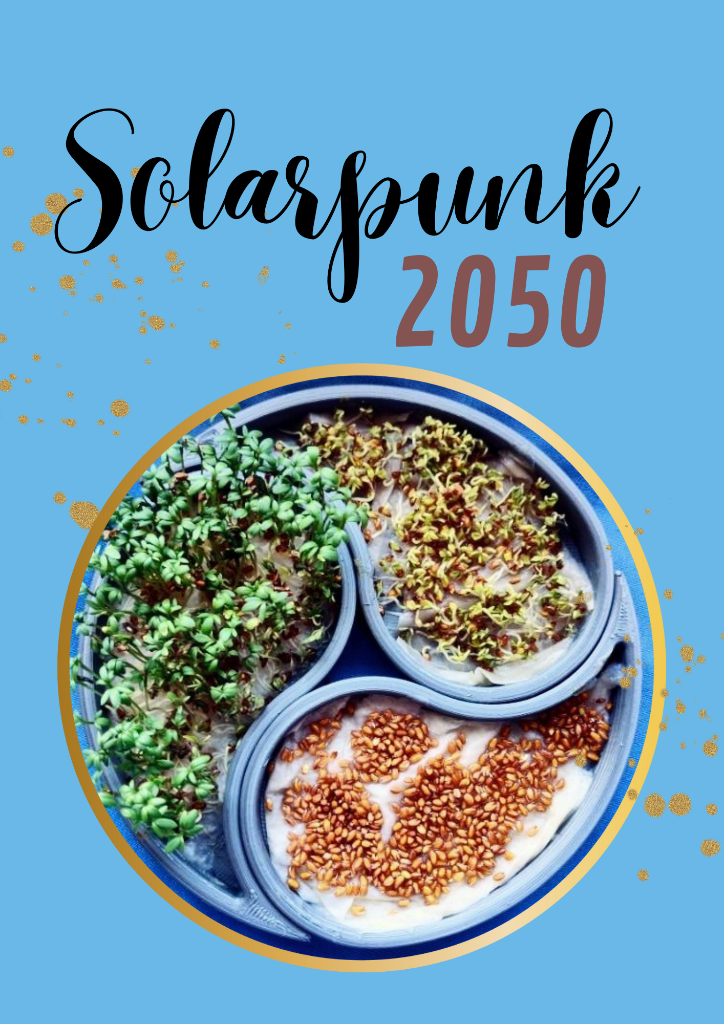
\includegraphics[width=\paperwidth,height=\paperheight]{static/title.png}}
}

% For creating example text
% \usepackage{lipsum}

\title{Fate Solarpunk 2050}
% \subtitle{A Solarpunk revolution}
\author{Thorsten Sick}

\pagenumbering{arabic}

% Index stuff https://www.namsu.de/Extra/pakete/Makeidx.html
\usepackage{makeidx}
% \usepackage{showidx}  % Shows index marker at page side
\makeindex
\begin{document}

%
% Book front page
%
\mbox{}
\thispagestyle{empty}
\BgThispage

\maketitle

\tableofcontents
\clearpage
\setcounter{page}{1}
\newpage
\begin{center}
\textbf{Dedicated to my friend Stefan, with whom I travelled through many worlds}
\end{center}
\newpage
\newpage
\begin{center}
\textbf{Text and idea}
\newline
Thorsten Sick
\newline
\textbf{Special thanks to}
\newline
the Solarpunk philosopher Pawel 'alxd' Ngei ( https://alxd.org/ )
\newline
\textbf{Test players}
\newline
Matze, Bene, Micha, Michael, Ingrid, Susanne Peschl, Christian "ChadTaranta"
\newline
\end{center}
\newpage
\newpage

Solarpunk is about community building. If you want to lift others up or get help, join our "Solarpunk" 2050 discord server.

\href{https://discord.gg/jPEPXzH7S4}{https://discord.gg/jPEPXzH7S4}.
  %% AI-ed
\section{Teaser}

A FATE Setting - It's the year 2050. The Solarpunks have saved humanity. And although now everything could be fine . . . isn't it.

The Solarpunks live their hyper-progressive technology utopia while the normal people think that we have already achieved enough by saving the world and that we can finally finish watching the latest series - the AI has at least marked it as a personal recommendation. And the lost want to go back to the 1990's as it never was. With added violence.

So the work of the solarpunks is not finished yet. And they are happy about that.

\begin{solartalk}[title=Solarpunk Photovoltaik site]
    Well folks. Unpack the soldering irons. We need a new autonomous solar farm for community expansion.
    We have 10 laser welding machines. Fits perfectly - so there's no dispute - this time all the children can help stand up the solar modules. Who is securing the perimeter with the drones this time? Yesterday someone heard diesel engines in the forest.
\end{solartalk}

\begin{solartalk}[title=Solarpunk Photovoltaik site - later]
    \begin{itemize}
        \item \npcquote{Drone Pilot}{Folks, I don't see any casualties, but we have a problem}
        \item \npcquote{Benjamin}{Are the children okay?}
        \item \npcquote{Drone Pilot}{Yes. No one was hurt. 10 with laser welding devices, 5 with their children's exoskeletons constructing the solar modules. But they 're doing too well.}
        \item \npcquote{Benjamin}{?}
        \item \npcquote{Drone Pilot}{From above, the modules look like a giant penis. Time to penis of 5 hours is impressive perfomance. But I'm for house arrest}
        \item \npcquote{Benjamin}{I wouldn't give one for that. When I was young I went through a phase where I drew stuff on bus stops with permanent markers}
        \item \npcquote{Drone pilot}{But you can see him from space !!!}
        \item \npcquote{Drone Pilot}{. . . Tonight at the community meeting. We need to talk. . .}
    \end{itemize}
\end{solartalk}

\begin{normtalk}[title=Party chat]
    \begin{itemize}
        \item \npcquote{Tscharlien}{Found something in an underground forum. For the episode 5 season 6 of Woodland Village you should buy the Mykonos inc red wine, the Mykonos inc olives (black) and the Mykonos inc feta. Why it didn't say.}
        \item \npcquote{Mischell}{I read that too. Unfortunately did not do that.}
        \item \npcquote{Kewin}{I saw that too. Why should I have done that ? Missed the episode.}
        \item \npcquote{Tscharlien}{That was so awesome!!! So great! So the gang in the episode sat there at the table in this fine pub between 1:45 and 2:15 and ate exactly the same things! I felt like I was there!}
        \item \npcquote{Mischell}{I saw that too. Will always regret not belonging to the underground forum.}
    \end{itemize}
\end{normtalk}

\begin{losttalk}[title=Council of war]
    \begin{itemize}
        \item \npcquote{Brutus}{According to our scouts, the Solarpunks are celebrating their new crazy thing: a giant Solar Penis. While the weirdos are distracted, we'll raid the Norm City}
        \item \npcquote{Achilles}{A what ?}
        \item \npcquote{Brutus}{The Plan: Motorbike Phalanx to the marketplace. Artillery at the city limits. Flanking from Greengate Park and from the ice cream parlour.}
        \item \npcquote{Achilles}{By the way, the can artillery people are sober again}
        \item \npcquote{Brutus}{Good}
        \item \npcquote{Brutus}{Then we'll get the most important BBDs out with the trucks and be gone within an hour. By then the police will arrive from the next town or so.}
        \item \npcquote{Achilles}{How much beer, beans and diesel can we get in the truck in an hour?}        
    \end{itemize}
    The conversation is interrupted by a test shot from the can artillery, which hits the tent. No injuries        
\end{losttalk}


\begin{normtalk}[title=Defenses]
    \begin{itemize}
        \item \npcquote{Supervisor}{Chief Inspector Dehnis? The Lost are attacking the city. Your troops have order to retreat so as to not to further provoke the Lost}
        \item \npcquote{Chief Inspector Dehnis}{Understood}
        \item \npcquote{Supervisor}{Are the warehouses sufficiently stocked with diesel, beer and beans?}
        \item \npcquote{Chief Inspector Dehnis}{Yes}
        \item \npcquote{Supervisor}{Well, then it should be over soon. By the way, reinforcements are on the way. Meets in 1-2 hours}
        \item \npcquote{Supervisor}{And make sure the Solarpunks don't interfere. If necessary, encircle and seal them off. They will try to save the city again. I don't want to have to work overtime today.}        
    \end{itemize}
\end{normtalk}


\begin{solartalk}[title=Gathering]
    \begin{itemize}        
        \item \npcquote{Bernd}{Guys, short party break. The city is attacked by the Lost. We'll have to save it. The police have cordoned off the streets. So we race through the forest with the e-bikes.}
        \item \npcquote{Bernd}{The angel system is currently being updated. Everyone who wants to join assigns to one of the five teams. Details are in the angel system.}
        \item \npcquote{Bernd}{The Lost are after BBDs. In addition to protecting people and the city, we ensure that the diesel tanker does not leave the city.}
        \item \npcquote{Bernd}{The tanker must not burn out under any circumstances. The last time we compensated CO2 for 2 years. And that's why Team Five is the Hazmat Team. Only people with the necessary training can register there. This team always stays with the tanker. Don't forget the equipment!}
        \item \npcquote{Bernd}{Well. The task tickets are online. Everyone takes up to three tickets with tactical objectives and let's go.}
        \item \npcquote{Bernd}{The rest keep partying. We'll be back in three hours at most.}        
    \end{itemize}
\end{solartalk}
  %% AI-ed
\chapter{Genesis}

It's the year 2050. The last few decades have been a wild ride. Especially after people realized that they have to manage several catastrophes in parallel and that the simplest solution is to rebuild society as a whole, it was: Do or die trying.

They did it, they survived. Most of them.

Thanks in particular to the Solarpunk Communities. Solarpunks are people who have started a revolution with extreme out-of-the-box thinking and technological/ecological awareness. In their communities - almost self-contained experimental laboratories - they were experimenters and guinea pigs at the same time. And the general public called Norms watched curiously, fascinated and hoping. They integrated the most successful approaches into their own life and upgraded their cities to match the new reality.
As a result, society in 2050 at large is CO2 neutral, fairer, more peaceful and more open.
The Solarpunks saved the world - and yet they can't stop being the incubator for epochal upheavals and mistakes.
The Norms benefited. The Solarpunks are still running after reaching the goal. And a third fraction got lost on the road to transition - the so called "Dirty road to Eden". The Lost saw the price that will have to be paid and did to aggree with it on a moral level. Instead of pushing for a new future they oriented towards a past. Or a mix of the old epochs of humanity. They life in the ruins caused by catastrophes and the transition. They are gathering and reusing old tech, are survival experts, fighters and historians.
While the Solarpunks and the Norms prefered to forget the recent history, the years they all used to shape the future. Because some things are better forgotten.  %% AI-ed
% small_world
\chapter{Factions}

There are three major playable factions in the Solarpunk world. Each has its own unique approach to life.

\begin{itemize}
    \item The creative and forward pushing Pioneers
    \item The Norms, who draw their strength from cooperation as a collective society and AI coordination.
    \item The Lost. Digging in the ruins of the old world and improvising with the old technology.
\end{itemize}

These factions are not enemies. And a successful team will probably need members from all three factions. But there is always some friction between the different approaches these factions have to life, the universe and everything.

The reduction to three factions is not the whole truth. In 2035, the faction construct was created by sociologists using cluster analysis to somehow label modern societies. There are even more factions than that if you start counting the small and odd ones.

The factions are also fluid. Members of a family may belong to different factions. Or a person may move from faction to faction as their outlook on life changes. This is not a big deal.

Factions are not strictly defined. There are hundreds of different Pioneer communities, each with their own approach to experimenting with a possible future. Hundreds of AI-powered cities where the AI will shape society differently because of the local definition of a "happy life". And many Lost Families who have found their own way to survive and thrive in the wilderness.

GMs and players: Create your own !

The Solarpunks: This game is set in the midst of the Solarpunk revolution. No faction can call itself Solarpunk. Each lacks some of the core principles that make it Solarpunk. But if the factions were to combine their strengths, they would evolve into a Solarpunk movement. This development could happen in the group of protagonists, in the communities they create and in the people they meet.

Because:

\begin{itemize}
\item The Lost lack the openness and progressive spirit of the Pioneers.
\item The Pioneers lack the wisdom of the past that the Lost collect.
\item The Norms lack the spirit and curiosity of the Pioneers.
\item The Norms could teach the individualistic Pioneers a thing or two about cooperation.
\end{itemize}
  %% AI-ed
\chapter{Start Playing}

You have just learned the basics and the factions. This book is designed as a tutorial. And you should start playing now.

Decide who will be the GM, let them jump to the first adventure. All the information you need is either in the adventure or linked from there.

The quests come with ready-made characters and the first ones only focus on small parts of the world. A manageable part of the whole sandbox.
Specific themes in the adventure are linked to the detailed description in the sourcebook. The GM can prepare as much as she wants.

This is the way the book is meant to be used.

\section{Adventures}

The first batch of the adventures is set in southern Germany, at the Lake of Constance. 2023 this region is rural with small towns and high tech industry. A good foundation for all the factions to start rebuilding after the disasters.

\begin{itemize}
\item \hyperref[ch:the world destroying machine]{The World Destroying Machine}: Play the Pioneer faction. Learn about the world and the factions
\item \hyperref[ch:project lifeguard]{Project Lifeguard} Play all the factions. And uncover the secrets of Project Lifeguard
\end{itemize}  %% AI-ed
\section{Pioneers}
\label{sec:Pioneers}
\index{Pioneers|(}

The Pioneers took the future into their own hands. They saved everyone and the planet, and now they draw strength from that.

Hardcore Pioneers are only a small part of the population (and this can vary locally). But because they actively participate in life, they are the part that leaves its mark on society.

Their main goal is to develop a modern lifestyle where humanity, nature, technology and spirituality are in balance and much more advanced.

Their communities are a place to experiment with new ways of living, energy production, society, spirituality and food.

Most of the objects are prototypes and experiments. Almost everything is unique and built from scratch.

Sometimes they succeed in their experiments. Sometimes they fail horribly.


Daily life: Pioneers spend their time doing what they love. Tinkering for 10 or more hours a day is not uncommon. They often change projects once a month. If someone runs out of projects, tasks can be found in the local computer system, where anyone can post things that need to be done. There is no payment, but there is an unofficial currency: respect. This can be earned through achievements or contributions to the community. This \hyperref[sec:meritocracy]{Meritocracy} results in people with high levels of respect being able to attract more people and resources to their next project, or being the centre of attraction.
Going on an adventure to serve the community could also be a source of this respect.

\subsection{Cyberware}
\index{Cyberware}
\label{sec:Cyberware Pioneers}

Pioneers never manage to get the complex infrastructure for building and implanting cyberware up and running. It requires hundreds of specialists and is just boring. This is a task for the \hyperref[sec:Cyberware Norm]{Norm} Society.

But they love to tinker with cyberware that is already installed. Add a few extra sensors, overwrite the firmware. This can unlock new features and also introduce glitches.


\subsection{Skill: Prototyping}
\index{Prototyping}
\label{sec:Prototyping skill}

Pioneer technology is unique. They find intelligent solutions to problems. They tend to build prototypes that will never be used in mass production.

These prototypes are built quickly, solve a problem, use available technology and will never get a safety certificate.
Often they are not meant to last.
If a pioneer has to build the same technology a second time, it will be built with additional features or a different approach.

Use the Prototyping skill for this type of dirty engineering.

If non-renewable resources are needed, also roll for Resources.

\subsection{Economy: Meritocracy}
\label{sec:meritocracy}
\index{Meritocracy}

In the Pioneer world, your reputation is the key that unlocks doors. People who trust you will give you access to resources, join your projects or simply believe you.
Anyone can earn a reputation by building projects, organising parties, surviving an adventure, or simply being the best person to talk to when someone needs a problem solved.

\subsection{Food}
\label{sec: pioneer food}
\index{Food!Pioneers}

There are two types of food you can find in a Pioneer community.

\subsubsection{Party food}

Pioneers like to experiment with food. They first invented hydroponic gardens, which are now used in Norm's hives. They also invented in-vitro meat. But they were never interested in scaling it up. Instead, they experimented with new cell cultures and tissues. Pre-seasoned meat is also a thing.
Insects piqued their interest (because they grow quickly and the project cycle time is short). Yeasts - which can be genetically modified to produce a variety of different flavours and substances.

It is hard to eat the same dish twice when visiting a pioneer community. They are constantly improving their recipes.

In practice, food is free because there is always a kitchen experiment going on that needs testers and tasters.

Pioneer food is always unusual and surprising. There is a risk that the experiment will go wrong, which could result in terrible food or some health risks.

\subsubsection{Tinker food}

Tinker food is easy to prepare and eat. It is meant to be eaten while a Pioneer is hacking in a flow that can last 20 or more hours. Typical Tinker food is Flavour Balls. Pea-sized balls of any flavour. These dried balls just need to be watered and grow to table tennis ball size. One is sufficient for the next 4-6 hours. And contains plenty of guarana.
Typically, a pioneer will put one in their mouth and sip coffee to let it grow in their mouth. It is not recommended to take more than one.

\subsection{Tech level}

Experimental technology. Things that were prototypes in 2020. Nothing boring

\subsection{Music}

Pioneers love music called "nature core". These songs go from idyllic to noisy/extracting and back to idyllic again. But the most unique feature is that the songs are generated by algorithms fed by listener behaviour.
The song is different every time you listen to it. But the algorithm used to generate it still makes it different. So musicians encode these algorithms and advertise them. At rave parties, the dancers and party-goers are the "musicians".

\subsection{Opinion: Eat the Rich Festivals}

"I was there. I wanted to work for the billionaires and get my brain implant. There was a party while I waited for my number. But I guess there were too many people applying. I never got the implant. But the food was good. Now that I am older, I do not know if I would try it again. But maybe I should try to recreate the recipe for the sausage. Yes, I know what they say was in it. But I don't believe it."

\subsection{Law}
\label{sec: pioneer law}
\index{Law!Pioneers}

\subsubsection{Important Pioneer laws}

\begin{itemize}
\item{Never commit Resource Point fraud}
\item{Never murder anyone}
\item{Never sabotage anyone's project}
\item{Always share your knowledge - but you can keep 8 of your inventions/innovations a secret}   % 8 = 2³
\end{itemize}

\subsubsection{Investigation}

In a very uncoordinated way, everyone will be running around collecting facts. These will be entered into a wiki.

\subsubsection{Jurisdiction}

Judgement is a democratic exercise. Anyone can vote digitally after reading the wiki.

\subsubsection{Punishment}

Punishment depends on the crime and the percentage of votes for "guilty".

The harshest punishment is forced sharing of technology and innovation secrets. This can go up to all 8. After that, the guilty must innovate to rebuild a stock of uniqueness.

The second harshest punishment is to leave the community and travel to other communities to spend time there and get enough "has been a perfect contributor to society" signatures. Doing specific projects there or contributing to society for a few months will do the trick. Depending on the verdict, the offender will need more or less signatures to return. In the end, the offender will have learned a lot and will have the chance to be welcomed back into their old society.

\index{Pioneers|)} %%  AI-ed
\section{Norms}
\label{sec:Norms}
%% TODO : Add hedonistic sustainability https://de.wikipedia.org/wiki/Amager_Bakke
\index{Norms|(}

Norms live in retrofitted cities with added solar panels, green parks, small streams and lakes. It is all quite idyllic, but you can still see the original buildings from the year 2020 beneath the green walls.
Because modern Norm tech is built using templates, many items, clothing, fashion and architecture look identical. These templates can be personalised. And smart people do. But they will never achieve the creative chaos of the Pioneers.

The cities are known as 'hive cities', and Norm society is often referred to as a 'hive'. The reason for this is the tight and close coordination of this society.

This society is coordinated by AIs (one per city) with the aim of improving the quality of life for the inhabitants.
To measure this quality of life, each norm carries a "hive controller". A communication device with an AR interface. This is also the main tool they use to work their magic: "hive control".

Someone from 2020 would call them magicians. Using augmented reality apps on their hive controllers, they can request services from the AI. These range from ordering refreshments to building a house.
Based on available templates, the AI will coordinate factories and Norm contractors (very specialised ones) to build and deliver the customised request by drone.
Delivery can take anywhere from a few minutes (ordering a pearl-gripped weapon) to a few days (adding a house to the city), as long as the Norm user is within the city limits.

This ability is not limited to physical things, but can also be an app to organise a party for 500 people.

But there are limits:

\begin{itemize}
    \item Extraordinary things cost money. And material things also cost resource points
    \item Apps must first be unlocked by successfully completing a tutorial. This can take up to 2 years for a complex architecture App.
    \item This magic will only work in the control area of an AI. And the supply lines must be open. The app will indicate when a service is unavailable
    \item Some high-risk services may also require a medical, age or other additional certification. This includes drinking alcohol and caffeinated drinks.
\end{itemize}

AI-controlled hives are networked. And a traveller can get similar services in most connected AI Hives.

It takes time to complete the tutorials and requirements for the most complex apps - most norms focus on 1-2 topics and the usual 40 apps everyone uses to make life easier.

A visiting Pioneer or Lost can get a hive controller, but will start at rank 0 (infant). They will only have the basic apps (pizza service, ....) and no idea how to use them. Completing the basic tutorials will take some time.

The real stars of the Norm world are those who can create new templates for new services. And only a few geniuses can create templates for highly complex products (like trains).
These templates and their apps unlock new wonders for society and make their creators famous.

Appearance: Compared to the world of the Pioneers or the Lost, the world of the Norms is uniform (thanks to the templates). Everything is mass-produced with some added personalisation. This includes solar upgrades to houses and clothing.

However, there is a certain dynamism to the cities, due to the plants and animals that have been allowed to proliferate.

Mobility: Mass transport. But with added quality of life (the self-driving tram has a bar and a big TV screen for entertainment. People stand in groups chatting and enjoying the ride).

Daily life: Work is optional. All \hyperref[sec:basic income]{basic goods are available for free}. If someone chooses to work 25 hours a week, they will be paid in local euros or other local currency. This can be spent on premium products and services. Jobs are very specific (like drone pilot for food delivery, barista or med-tech). People tend to have at least 1-2 hobbies that they are very good at in addition to their job.

Norm society depends on a warehouse sized AI controller with communication interfaces in the city.

To spread Norm society to new cities, the Norms usually start with a shipping container containing AI, communication interfaces and power. These "seed hives" have limited capabilities, but are sufficient to bootstrap a new society. The AI inside is created from an empty template and can adapt to the situation. When set up, the AI will establish a radio link to a partner city's hive and begin building an inventory of local services and people with a hive controller in their area.

A Norm on expedition can still have some advantages by using a 'personal hive', which is just a long range communication interface to the nearest city hive. With all the negative effects of: lag, broken connection, slow delivery...

\subsection{Hive controller}
\index{Hive controller}
\label{sec:Hive controller}

The Hive Controller is a headset used for communication. It also has an AR interface that projects menus in front of the user. These can be controlled by touch. This device makes the user part of the social and technological network of a Norm Hive.
It is used to communicate, plan, organise and order things.
The Hive Controller has a number of sensors that can measure the environment or the user's health. In this way it can guide the user towards a healthier lifestyle.

It also handles payment for premium services.

A special skill is required to operate it. These are acquired and improved by Norms by completing the tutorials in the apps the Hive Controller has. More and more functions are unlocked, starting from the Norm's childhood. Obviously: When a Pioneer or Lost receives a Hive Controller, they must start with the most basic tutorials.
Sometimes applications are updated with new features. This may also mean that users will need to complete another tutorial before they can continue to use that application.

\subsection{Cyberware}
\index{Cyberware}
\label{sec:Cyberware Norm}

The Norms have a very advanced medical system. Anyone can receive free medical care and therapy. Cyberware replacement until limbs grow back is an option.
By law, cyberware is limited to the power of a healthy human. This is to prevent people from using Cyberware as an enhancement.

This medical excellence can only be achieved by a granular division of labour and a bunch of specialists.
Too boring for a Pioneer, too complex for the Lost. But people from these factions can also be treated in a Norm city. It may take some help to overcome the cultural differences. But there will always be someone who will - for a price.

There are rumours that the Pioneers hack already implanted \hyperref[sec:Cyberware Pioneers]{Cyberware} to remove the restrictions. But that would be illegal.


\subsection{The AI}

The AI at the centre of the hive is the same type of AI in most cities. It is not self-aware. Its planning skills are "high human" and at its core it is a statistical engine combined with a bunch of algorithms. Nothing magical. But as a central project manager with a "team" of specialists and experts the size of a city, it can work wonders.

It is also a force multiplier for local behaviour and traditions. As it optimises for "quality of life", it will support everything that local people see as positive and dampen everything they do not like. The cultures of Norm cities may evolve in different directions after a few years of AI control.

There are rumours that some hives, with the help of some Pioneers, have upgraded their AI to something more powerful and perhaps self-aware. But these rumours are most likely based on non-standard hive controller interfaces and a very strange local culture.

\subsection{Library of things}
\index{Library of Things!Norms}

Each hive has a library of items that Norms can borrow. They usually select them from the Hive Controller menu and have them delivered by drone. These items are not personalised. \textbf{Of course, they have to return them on time, unmodified and undamaged.} (unmodified is tricky if you have a Pioneer in your party).

\begin{normtalk}[title=Problem solved]
    \begin{itemize}
        \item \npcquote{Norm}{So this is where I scripted the library of things. The script runs every 10 seconds, filters for 'clothes', sorts by 'colour'. And if the availability of any colour suddenly drops, I get a fashion alert on my Hive Controller and can go emergency shopping and borrow clothes in the current fashion colour.}
        \item \npcquote{Pioneer}{With all due respect for your technical prowess, but can you please tell me: What is the problem you are solving? I don't get it?}
    \end{itemize}
\end{normtalk}

\subsection{Skill: Hive control}
\index{Hive control}
\label{sec:Hive control skill}

Being near a hive and having a hive controller allows a Norm to request services from the hive. This is done using the Hive Control special ability.

The target that needs to be rolled depends on the complexity of the task the norm is trying to accomplish.

Sometimes an additional resource roll is needed to check if the norm has the resource points for the non-renewable resources they need. Most of the time the hive will try to help by allowing the user to borrow a similar item from the hive's library.

If the hive control die roll fails, this may be the reason:
\begin{itemize}
    \item User must complete some tutorials first
    \item The app has been updated ....
    \item The hive is busy and this request cannot be queued yet.
    \item Basic components must first be shipped from another hive
    \item Hive controller down (this is an emergency!)
    \item You have just been given a task for your daily work...
\end{itemize}

AI controlled areas can be in 4 quality ranges:

\begin{itemize}
    \item City hive: no penalty
    \item Seed Hive (AI size: one shipping container) -2 to throw, slow delivery
    \item Personal hive (just a good communication interface to the nearest hive): -4, slow delivery
    \item No connection: Sorry.
\end{itemize}

Most people in a Norm society choose to have a job. This will keep them busy for about 25 hours a week. These jobs are coordinated by the AI (a society-wide project management software). It can happen that the Norm character who is adventuring somewhere will be assigned a job ticket at any time: ....

\subsection{Economy: Basic income}
\label{sec:basic income}
\index{Basic income}

The Norms have done little more than tweak the monetary system. The big thing is: Everyone has a kind of basic income: What you need to live is free.
You only pay for premium items. That way, people with jobs can get some motivation out of it.

Every person (not only Norms, but also Pioneers and Lost) can just take the basic goods in a reasonable amount. This includes:

\begin{itemize}
    \item Food
    \item Drinks
    \item Clothing (basic)
    \item Shelter
    \item Public transportation
    \item Cultural participation
\end{itemize}

There is also a 'premium' version of all these goods that you have to pay for. This version is somehow extra fancy. As a reference: Free-to-play games where you can buy extra gadgets without any gameplay effect. That's common in 2020.

The basic income is not paid into your bank account! Instead, there are shelves/vending machines and other places in the cities where you can just grab what you need.

Example of a premium: Near the free coffee machine there could be a real person barista making great coffee and offering a nice chat for some money you earned at your job.

This basic income is possible because renewable energy is unlimited, production is automated and so is logistics.

\subsection{Work life balance}

Some Norms decide not to work - which is totally accepted in this society. They can access alle the basic goods and services for free.
The more active Norms decide to have a job keeping them busy for 25h per week. This is how they earn money for premium products. No matter which approach the Norms take: There is plenty of time for hobbies. And everyone who is not passively consuming will dedicate their spare time to hobbies like:

\begin{itemize}
    \item Alternate reality spy games
    \item Swashbuckling
    \item Reenacting films
\end{itemize}

This leads to Norms having some very strange skill sets or stunts.

Besides: Norms without a day job could be very tempted to commit to an adventure if money can be earned.

\subsection{Appearance}

Off-the-peg clothes are not changed every season for ecological reasons. However, there are many accessories that you can use to show your affiliation and your knowledge of fashion. Often adapted to match the dresscode of the current favourite movie star.

\subsection{Housing}

Norm Hives are either built on top of old cities using mass-produced green technology (like solar panels), or built from scratch using standard building modules, with lots of greenery in between.
Everyone is given free access to their own small apartment - which they can move out of at any time. These apartments are fairly empty, but have a drone docking port on the wall. Whenever you need something, you can order it with your Hive Controller and it will be delivered to your apartment within minutes.

One room per person. In addition to the standard bathroom and kitchen. Families are given multi-room flats where they can remove the partition between the rooms.

There is no furniture in these rooms. But using the Hive controller app, you can configure the flexible floor and wall elements to form chairs, beds, sofas and tables wherever you want or need them.

Thanks to drone delivery of everything you need straight to your home's drone docking port, owning stuff feels like a burden to Norms. Many Norms have only one bag of personal belongings. This allows them to move to another apartment in another part of the city with ease.

When the Norms have finished using the borrowed items, they simply drop them into the out-box of their home's drone docking port and they are returned to the central warehouse.

\subsection{Communication}

The Hive Controller allows instant communication with other Norms in the same Hive. Everyone is online. All the time. Some hives have even managed to connect to other hives and their virtual communities have merged.

\subsection{Food}
\label{sec: norm food}
\index{Food!Norms}
\index{Ceres}

Food production is industrialised and automated in a so-called "Ceres" (Ceres is the Roman goddess of agriculture, but no Norm will care where the name comes from). Old factories have been converted into these agricultural factories. Plants are grown in in-house vertical gardens, tended by robots.
Meat is produced in vitro, where a cell culture is simply given energy and nutrients to grow into a steak. Much of the food is also bar-sized and the ingredients are produced by algae and yeast grown in large tanks.
Dairy products are also produced in tanks from cell cultures grown in the lab. Starting with milk (cow, goat and tiger flavours are common), which is the base product for yoghurt - and which is made from milk with microbiota as in the old days.
Fruit from large plants is also grown from bioengineered cells - which produce fruit pulp in a tank. This pulp - mango in this case - is then pressed through a mango extruder to form a rod - a few hundred metres of mango. This is then sliced, dried or diced into yoghurt and that's it. Tiger Mango Yoghurt is hip in 2050.

Everything is tasty, but according to the Pioneers, this food "lacks that special something".
This food is free and can be obtained from either automated kiosks or cantinas. But each Ceres also has an attached restaurant where you can get it directly from a robot. A Ceres is designed to be open to visitors, and anyone can verify that the food has been grown in a hygienic way.

If you want to eat premium food, you can go to a restaurant (which often shares parts of the kitchen with a free cantina). Here the same ingredients are cooked by chefs. Properly seasoned and served with the perfect wine. With a Hive controller, you can even specify the matching tablecloth and a scented candle to whet your appetite.
Sometimes you will meet a salad sauce sommelier who can help you define the perfect sauce for your dish. The recipe is stored in your Hive Controller. This is a premium service, of course, but well worth the investment.

Of the food options offered by the factions, Norm Food is the least spectacular and most boring. But tasty. On the plus side: There is zero risk.

\subsection{Tech level}

Mass produced technology. Things that will be prototypes in 2020. Nothing daring. A Solar IKEA-isation of cities.

\subsection{Music}
\index{Music!Norms}

Music is pop music taken to the extreme. Maybe a hundred experts work on a new song, starting with social studies. All this data is fed into a pool where people create songs that fit the general taste of music. Well-known songs are reproduced, but with tiny improvements. Listeners will not know if they have heard this song before or if it is new. But the Norms love it.

\subsection{Opinion: Eat the Rich Festivals}
\index{Eat the Rich Festivals!Norms}

"Yeah. I still love that. A perfect trope. Almost all the films based on the Eat the Rich Festival theme are great. I think they should make more. I have no idea what really happened to the billionaires. But for entertainment purposes I fully support the festival theory.

\subsection{Law}
\label{sec: norm law}
\index{Law!Norms}

\subsubsection{Important Norm laws}

\begin{itemize}
\item{Never commit Resource Point fraud}
\item{Never murder anyone}
\item{Never spoiler an unreleased story}
\item{Never break a \href{https://en.wikipedia.org/wiki/Kayfabe}{kayfabe} - a staged event meant to entertain the audience}
\end{itemize}

\subsubsection{Investigation}

In most cases, the investigation could be simple. The AI that monitors the Hive already knows who did it. But for security reasons it is programmed never to tell anyone. Instead, investigators are sent out to gather the pieces of the puzzle and reconstruct the crime.
What makes Hive investigations so special is that the AI can send out clues and cryptic messages. And if the criminal kills the investigators and there are witnesses, the case is solved as well.

\subsubsection{Jurisdiction}

Once all the fields in the investigation form have been filled in with facts, the AI will immediately send a judgement report.

\subsubsection{Punishment}

As punishment, access to Hive features can be restricted, and a mandatory 'probation officer' app will guide offenders back into society. In the process, some apps and features will be unlocked. The probation officer app may ask for seemingly absurd tasks, but some may just be designed to trick the offender into meeting the right people (while the task itself is irrelevant), or being in the right place at the right time. Destiny encoded.

\section{Micro missions}

Part of the Norm economy is what are known as "Micro Missions". While walking through a Hive, a Norm can see an indicator for these micro-missions pop up in AR.
The average time to complete them, the skills required and the reward are also shown.
Most of them have a small tutorial video explaining what needs to be done. As soon as the Hive marks them as completed, the money will be transferred.
Anyone with a Hive Controller can create Micro Missions.
Typical Micro Missions are
\begin{itemize}
    \item The sensor on this bin is down. Check it. You will receive a replacement via drone. Installation is easy. 10 minutes, 15 euros
    \item This cafe needs to move its tables outside, the location can be seen in the video. 6 minutes, 5 euros
    \item Strange noises have been reported coming from the sewers. Open the crate so the drone can drive straight in. 3 minutes, 4 Euros
\end{itemize}

Most unskilled, repetitive, short and simple tasks in a hive are scripted this way. Some people have no day job, but spend about an hour a day doing these tasks and are done with making money.
%% TODO specific crimes: Spolering episodes, den make-beliefe brechen (check wrestling) Kayfabe

% TODO: Add example stunts
\index{Norms|)}  %% AI-ed
% Checked by Editor
\section{Lost}
\label{sec:Lost}
\index{Lost|(}

The Lost are the faction that did not join the others on the "Dirty Road to Eden". They realised early on that there would be some horrors involved in achieving a solarpunk utopia. And they were not willing to pay the price. This faction is the only one that does not actively deny what has happened.

Their approach is to live in and from the ruins of the Lemmings' civilisation. They reuse, recycle and upcycle the old technology. This is what their clothes, tools, vehicles and shelters are made of. Old technology reused in creative ways. Most of it looks shaggy.

Living among the ruins, they have developed fighting and survival skills and are experts at exploration.
Many are historians, collecting ancient documents for their secret "Alexandria" project.

Daily life: The Lost are constantly fighting for survival. Either by gathering food in the wilderness or in the ruins, or by repairing old technology. Some tend farms. Others run shops or try to keep truck stops alive to provide some sort of safe travel through the wilderness. Their internal trading system is a \hyperref[sec:Barter]{barter} system, so they trade items for other items, food, information or fuel.
The Lost gain resource points like everyone else. But they tend to spend them on the privilege of burning fuel. This forces them to scavenge the ruins for resources to upcycle or recycle (for Resource Points).

Their reliance on old technology makes them the only faction without drones. They are also the only faction to have trained animals.

\begin{itemize}
    \item Search, rescue, hunting and cart pulling dogs
    \item Horses for riding and transport
    \item Rats for substance detection, food testing and rescue
    \item Birds (eagles, falcons, owls for hunting or reconnaissance, homing pigeons)
    \item Dolphins and seals.
\end{itemize}

Some of the Lost developed an almost mystical relationship with their animals. At least according to their Norm friends who grew up in cities.

The Lost do not necessarily trust the Pioneers or the Norms. They remember the "Dirty Road to Eden" well.

\subsection{Shakespeare battle}
\index{Shakespeare battle}
\label{sec:Shakespeare battle}

Despite the rough first and second impressions they make on outsiders, the Lost are educated and hold history and old books in high esteem. The battle consists of one person starting to act out a scene from an old play and handing over to another person who must continue without fail. This is a drinking game and will turn into a chaotic situation.

(If the players' characters are part of the fighting crowd. GM: Bring a copy of a page from a Shakespeare play to play at the table).

\subsection{Skill: Bushcraft}
\index{Bushcraft}
\label{sec:Bushcraft skill}

The Lost know their way around wilderness and ruins. They can up-cycle and recycle old technology. They build camps, hunt, gather food, train animals and scavenge ruins for tools.

All of this is covered by the Bushcraft skill.

\subsection{Typical Lost protagonists}

\begin{itemize}
    \item Scrap collectors
    \item Indiana Jones-style adventurer
    \item Lost ranger and animal expert
    \item Survival specialist
    \item Librarian
\end{itemize}

\subsection{Traditions}

\subsubsection{Guests and weapons}
\label{sec:Lost guests and weapons}
As survival experts, helping people and providing shelter is a sacred tradition. People who come in good faith are given shelter, food and medical care (Lost medicine is mostly rustic first aid).

But before entering a Lost camp, guests are searched for weapons. If they do not have any, they will be given some basic ones to use for the duration of their visit. They can also receive basic weapons training. The Lost expect their guests to help defend their camp if it is attacked by critters or other humans. Guests are therefore armed.

If guests are not trustworthy, they will not be given ammunition for their weapon - until their help is needed to defend the camp.

\subsubsection{Libraries}

The first impression other factions have of the Lost when they first meet them is that they are an uneducated bunch of survivalists and fighters. Once they get to know some of the Lost, they learn of their true mission: to protect the past. They collect old books (from phone books to the Luther Bible) and art (from everyday objects to old paintings).
These are stored in the mobile library that most Lost families carry with them (a steel box in the boot or a special armoured bus).

Books that are not yet in Alexandria are sent there on a pilgrimage. It is a paper-chase adventure with missions at each stop. The official aim is spiritual experience and growth, which may lead to some of the participants becoming librarians of Alexandria. The unofficial goal is to hide the current location of Alexandria from anyone following the group.
Groups travelling to Alexandria will be secretly monitored by experienced Librarians. Anyone following these groups will be dealt with.

For most of the year, Librarians live with a family. Only when Alexandria is established will they be called upon to leave the family for a few months.

Alexandria is a library built out of shipping containers. To protect it, it only exists for a few weeks a year. Its location is a secret known only to the librarians. Pilgrims are led there by the Paper Chase. The containers contain the library's books and index.

When a group of pilgrims arrives, they hand over the book, which is then indexed. Skilled forgers make exact duplicates, which are sealed with the library's seal and returned to the pilgrims. Each pilgrim can also choose a book from the library. One copy will be mass-produced (using an ancient printing press) and returned with the pilgrims to their family library.
In this way, knowledge spreads and a decentralised backup is created.

All the Lost know of the Library. But only a few outsiders - those who have saved the life of a Lost and found a book not yet in Alexandria - are asked to join a group of pilgrims under a vow of secrecy.

\subsubsection{Librarians}

A pilgrim can apply to become a librarian. As well as being able to quote from 50 books, a librarian must be able to demonstrate special skills that the library needs. These range from forger, fighter (to protect the library), treasure hunter, builder (to rebuild the library once a year) and cook (to help with the pilgrims' gathering).
Part of the initiation ritual is to tattoo as much text as possible from the new librarian's favourite book on his or her body. People who know (this is mostly Lost) can recognise a Librarian by the letters tattooed on their skin.
Skin that cannot be hidden will remain free of text.

\subsection{Economy: Barter}
\label{sec:Barter}
\index{Barter}
The Lost spend most of their resource points on diesel. This is one of the reasons why they loot old ruins for materials and technology that they can up-cycle. This way they do not have to spend RPs on products.

They also have an internal barter system where they trade goods for goods (a chicken for this hammer...).
It is much more complicated than money, but they lack trust in other systems and it is transparent. So it works for them. And most of the time they trade within the same family anyway.
And you can use the goods while you wait to trade them (eggs from the chicken).

\subsection{Food}
\label{sec: lost food}
\index{Food!Lost}

Lost are the hunters and gatherers. They cook whatever they find. The ingredients are animals, vegetables, herbs and tins from looted ruins. The kitchen is a campfire and a few tarps around it to collect the food they gather.

A good Lost cook is good at improvising. The same dish will never taste the same because the ingredients will vary. The cook's goal is to get as many nutrients into the people as possible. Starting with the essentials like fat and other calories.

Cooking is usually done for the whole camp, including guests. They can also be recruited by the cook for simple tasks.

A very typical Lost dish is "Exhaust Bread", which is baked on the exhaust pipe of a moving truck.

\subsection{Diesel}

They burn diesel in their quest for independence and the "good old days". They spend all their Resource Points, which represent the resources a person can use without harming the environment. But spending these points also forces them to rely on looted and recycled materials. They cannot afford anything new. And they do not want to.
The other factions know this and don't see the social contract being broken. But they just don't understand the decision.

\subsection{Tech level}

"Nothing with transistors". Or better: Nothing that has a programmable logic. No solar power but diesel. By choice.

\subsection{Law}
\label{sec: lost law}
\index{Law!Lost}

\subsubsection{Investigation}

%% Elders are called together for the criminal case
%% Elders decide who will investigate

\subsubsection{Jurisdiction}

%% Elders receive info and judge

\subsubsection{Punishment}

%% People will be kicked out of the family. Can return after a Quest has been finished. This one is decided by the Elders. In a way of a "Hero journey" or "Finding my true self" journey from books

% TODO: Add example stunts




%% TODO: Add Flea markets as gathering
%% Todo: Opportunistic Waldgärten für Kartoffeln, Kräuter, Chilies: Lost are growing seedlings and planting them in small gardensto grow. If they find a garden they tend to it and harvest if possible.
%% https://en.wikipedia.org/wiki/Working_dog
\index{Lost|)}  %% AI-ed
% todo: example characters
% big_world

% todo: The Dirty Road to Eden
% todo: life
%humans_and_communities
\chapter{World}

The world in 2050 is a world that is being rebuilt after several disasters triggered by climate change and other human mistakes shattered it.

\section{Wilderness}

Large areas are uninhabited and turned back into wilderness. Some old towns are still there - ruins that are not claimed yet.

The humans found several new ways to life those are the \hyperref[sec: Norms]{Norms}, \hyperref[sec: Lost]{Lost} and \hyperref[sec: Pioneers]{Pioneers}.

Their settlements are the seeds from which a new Solarpunk world can grow.

\section{Climate manipulation}

\section{Relics}
\index{Relic}
\label{sec: Relic}
Relics are objects or organisations from the past. They do not fit into the new world and will be dismantled soon. But as there are any relics there is a long list of todos for dismantling. And some just soldier on until it is their turn. Or they fight back.

\section{UN}
\index{UN}
\label{sec: UN}

The UN is the only central organisation left after the catastrophe. They are the good guys leading rescue operations, rebuild and they also introduced the Resource Point system. After breakdown of the nations the UN had to be reinvented. As the organisation it should always have been.

Its missions:

\begin{itemize}
    \item Rebuild global communication using drones, zeppelins and glas fiber
    \item Build an economy based on recycling using \hyperref[sec:Resource Points]{Resource Points}
    \item Find and dismantle \hyperref[sec: Relic]{Relics}
    \item Re-connect settlements lost during the catastrophes to civilisation
\end{itemize}

The UN has a few bases around the world. But mostly efforts are franchised and specialists are hired for the specific types of jobs.

\subsection{Equipment}

The UN has some special equipment and personell at their bases.

\subsubsection{Cargo Zeppelins}
\label{sec: UN Cargo Zeppelins}
\index{UN! Cargo Zeppelin}
Large Cargo Zeppelins. Able to carry up to 4 shipping containers of cargo. The solar cells in their hull make them black, their electric engines silent. This has the side effect to make them mobile bases in secret missions. But the original idea is to be able to use them as floating power generators: They rise up to 500 meters, are moored to the ground and generate solar power for the ground part of the mission. In addition to that the engines can run in reverse and generate wind power.

\subsubsection{Away team}
\label{sec: UN away team}
\index{UN! Away team}
The away team can disembark from the Zeppelins using their E-paragliders and prepare the ground for landing the cargo or build an anchor for the Zeppelin. Those people are some of the best trained at the UN.


\section{Resource points}
\index{Resource Points}
\label{sec:Resource Points}
Resource points are the main currency accepted by all factions. To avoid abuse of the nature every person gets a limited amount of them each year from the UN. They are required to get any non-renewable material based object. The ones appointed are enough for a normal life style. But not enough to build a brewery. The only way to get more of those points is by recycling objects. You bring your old phone back to the shop and get qa new one. if you want more than just to replace your phone: Big objects or those made of rare materials return more resource points. This is one of the main reasons to start an adventure visiting the ruins of the Lemminsgs. The Resource Point system is maintained by the UN. 



\section{Kessler Syndrome}
\index{Kessler Syndrome}
\label{sec: Kessler Syndrome}
A mass crash of sattelites made the orbit around earth inacessible. There is are no weather satellites, GPS or map satellites left. No communication.
This is called "Kessler Syndrome". Leaving earth is high risk and no one tries that anymore.

As replacement people are using high altitude drone planes, baloons and zeppelins. They only cover a small region and must be started intentionally. But this is better than nothing. %% AI-ed
% \chapter{Economy}

\section{Resource points}
\label{sec:Resource points}
Resource points are the main currency accepted by all factions. To avoid abuse of the nature every person gets a limited amount of them each year from the UN. They are required to get any non-renewable material based object. The ones appointed are enough for a normal life style. But not enough to build a brewery. The only way to get more of those points is by recycling objects. You bring your old phone back to the shop and get qa new one. if you want more than just to replace your phone: Big objects or those made of rare materials return more resource points. This is one of the main reasons to start an adventure visiting the ruins of the Lemmings. 


\section{Lost: Barter}
\label{sec:Barter}
The Lost spend most of their resource points on gasoline. This is one of the reasons they loot old ruins for material and technology they can upcylce. This way they will not have to spend RPs on products.

In addition to that they have an internal barter system where they trade goods for goods (one chcken for this hammer...).
It is much more complicated than with money but they lack trust in other systems and it is transparent. So it works for them. And most of the time they trade within the same family anyway.
And you can use the goods while you wait to be able to trade them (eggs fromt he chicken).


\section{Norms: Basic income}
\label{sec:basic income}

The norms only did minory adjustments to the monetary system. The big thing is: Everyone has a kind of basic income: What you need for a living is free.
You only pay money for premium things. That way people with a job can get some motivation out of that.

Every person (not only Norms, but also Pioneers and Lost) can just take the basic goods in a reasonable amout. This covers:

\begin{itemize}
    \item Food
    \item Drinks
    \item Clothing (basic)
    \item Shelter
    \item Public transportation
    \item Cultural participation
\end{itemize}

From all those goods there is also a "premium" version you pay for. This version is somehow extra fancy. As a reference: Free to play games where you can buy extra gimmicks without any game effect that was common in the year 2020.

The absic income is not transfered to your bank account ! Instead there are shelves/vending machines and other opportunities in the cities to just grab what you need.

Example for premium: Close to the free coffee vending machine there could be a real person barista brewing awesome coffe and offering a nice chat for some money you earned at your job.

This basic income is possible because renewable energy is unlimited, production is automated and logistics as well.


\section{Pioneers: Meritocracy}
\label{sec:meritocracy}

In the pioneer world your reputation is the key that unlocks doors. People who trust you will give you access to resources, join your projects or just believe you.
Everyone can build a reputation by building projects, organising parties, surviving an adventure or just be the best person to talk to when someone needs a problem solved.

% \chapter {Solarpunks detailed}


\begin{warning}
    All the fractions get an adjustment. This includes the Pioneers. The details below are not verified and can be changed after some play testing.

\end{warning}

The Pioneers tackled the world's problems by innovation and set the foundation for the Norms to build on

\section{Profile}
\begin{itemize}
    \item Class: Meritocracy.
    \item Advancement in society: Successful and creative projects and campaigns
    \item Political System: Holocracy
    \item Form of society: extended family
    \item Conflicts: meritocracy bugs, urge for change
    \item Appearance: Self-tailored or fitted clothing. Very individual. Value is placed on practicability during projects.
    \item Taboos: idleness, stealing glory
    \item Language: Nerdy youth slang prevails
    \item Trends: progressive, creative, builder
    \item Law: * Judge: The group * Penalties: Community service to banishment from all Pioneer communities
    \item Corruption: Hardly. If so, then your own project may be supported with resources.
    \item Weapons: Elegant weapons are preferred. Because it is practiced as a sport: swords, bows (high-tech) and firearms, . . .
    \item Architecture: creative fusion with nature and technology. Community oriented. Very individual.
    \item Vehicles: Technologically very modern and digital, battery or hydrogen powered. Lightweight and small. E-bikes, e-cargo bikes, quads, exoskeletons
    \item Resources: There is a lack of large-scale industry goods. You're always chasing technology that you can recycle because you don't want to buy anything new (for ideological reasons)
    \item Celebrations: creative and rather small. With art and culture. In meeting houses or in the central square. Camp fires. Stories. Presentations of new projects. Theatre. Homemade music. Drone ballet in the night sky.
    \item Success: inventors of crazy technology, people who have performed a risky action
    \item Drugs: Used to be creative, happy and open. Enhancing ones. To boom and long-lasting influence is frowned upon. Because it paralyzes projects. Experimentation with intelligently designed and bred drugs is welcome.
    \item Psychotherapy: There are many educated, wise and pastoral people. Therapy is more of a sideline ongoing mentoring thing and no one really notices.
    \item Media: There are many very topic-specific podcasts/video casts and the like. Each created by our own experts. Lectures are also held and recorded. An immense knowledge archive is available. Art and culture are also recorded and distributed decentrally by communities.
    \item Education: flipped classroom, hands-on learning. No age limit for courses, but at best required prior knowledge as a limitation. Prior knowledge is managed using a badge system: https://support.mozilla.org/en/products/open-badges/introduction-open-badges .Teachers are recognized for their explanatory skills in their field. But not necessarily full-time teachers.
    \item Coordination: angel system. Tasks are entered into a system. If someone has time, they call up the tasks and sort them according to their skills/interests. Then do it and get points https://engelsystem.en/ An order in the Engel system can also be the practical part of a further training measure and be rewarded with a badge.
    \item Diet: Homegrown meat, vegetables. Creative cuisine is very welcome. And good Chefs can become stars.
    \item Names: nicknames, abbreviations, chat names, names referring to peculiarities. The names can often change in the course of life and are usually chosen by the person himself. Or earned
    % \item Gendern: With the -y ending and 'das' (after Phettberg)
\end{itemize}

Social: Sexually open (queer, trans, . . . ) and sometimes in polyamorous relationships. an entire community often identifies as one family and cares for the children (“It takes a village to raise children”).
The major disadvantage of this freedom, however, is the tension with more conservative sections of the population. Norms and Lost. Pioneers generally use the gender asterisk and the person's preferred personal pronouns. Many Pioneer communities are accessible as agrotourism for Norms and others to "experience" something.
Drugs: Light drugs are legal across the EU. Pioneers like to mix their own experimental stuff or grow mushrooms or hemp at great expense. Good drug experts are celebrated like artists.
Redemption: Some more subversive Pioneer groups feel they need to do the Norms a favor by tearing them out of the rut of normality. To do this, they plan subversive art actions, which they carry out at night and in fog to "open your eyes". The reaction of the norms and the AI (which wants to restore normality) is mixed and very unpredictable.


\section{Policy}
Communities are how Pioneers organize themselves democratically. These are self-governing structures that, at best, form a kind of communal village. But locally fragmented communities also exist and thrive. The form of democracy is a holocracy (https://en.wikipedia.org/wiki/Holocracy). Everything is organized in circles. These are linked hierarchically. The lowest level is a single project. After that comes the community, the local cluster of communities, the EU
representation of communities and then the global circle.
The members of the circles are democratically elected. In addition, one elected member is sent to the neighboring circles. That way everyone is connected. Another important principle: The circles do NOT try to find the best solution to a problem, but rather prefer the most easily correctable variant. This allows more experiments to be tackled.
A community lives according to self-determined rules. The standard Pioneer rules are their basis.
The basic set of rules for communities:
\begin{enumerate}
    \item Be excellent to each other!
    \item The community is democratic. Elections are held once a year
    \item These positions are to be filled: * Elder * Dispute mediator * Logistics officer * Quartermaster
    \item Nobody stays in the same office for more than 3 years
    \item The aim must be to fill the gender parity
    \item Refugees must be helped.
    \item The community must live and operate within natural limits. She must help others to do the same.
    \item Protective equipment must be worn in dangerous situations
    \item No biological experiments in the kitchen area!
    \item Who makes is right
    \item A competition between communities is a matter of honor
    \item Friday is pancake day
\end{enumerate}

The own community in which the characters live is itself a protagonist and is welcome to receive a character sheet. Growing it and making it more connected is a potential goal for players. But you also get direct benefits from new skills/ equipment from the community.
In addition, there are also regional customs between communities. Are known:
\begin{itemize}
    \item Sharing your own projects as a sign of trust. Two communities in the Black Forest exchanged the sourdoughs they had cultivated and optimized over the years. At first glance, this might seem banal. But they gave the other group years of work and a cultural uniqueness of their own. And in a reproducible form.
    \item Plant seeds as a welcome gift. Here, of course, attention is paid to special features and quality. 
\end{itemize}
Of course, this is also rooted in the "grow and let grow" of the solar punks.
For GM: These rules intentionally have some ambiguity. The story can then be hung up with that.
\begin{enumerate}
    \item Who is eligible to vote? Can you sabotage the election?
    \item What exactly do the offices do? Can one person hold multiple offices?
    \item And what if no good successor is found?
    \item How much leeway is ? How many genders are there?
    \item Fled from what ? The law ? How to help ? Also refugees from hostile groups?
    \item Purely theoretically: If you burn down a nasty industrial plant in self-defense, you have to compensate for the CO2. And whether others accept this help. . . 
    \item Protective equipment in the workshop is good. Here, however, it was forgotten that one must also be able to handle the devices. Especially with those that have been tweaked and customized by the community. . . 
    \item  Self-explanatory. But what if you have bred new brewer's yeast? When are they no longer experimental? 
    \item When someone proves that something can be done. Is he right? . . but can cause problems with very enthusiastic slobs can who challenge can't listen others
    \item to Communities compete. The winner gets clear reputation. The loser can also get points for a Grand Commendation to the winners. Both are archived in annals. The exact form of the competition is defined between the communities. => Start of many adventures
\end{enumerate}

\section{Holacracy}
Holacracy is actually a simple democracy with voting in small groups (that can be project groups, teams, communities). Since each group is networked with others, they send a kind of diplomat. This is why someone from the community leadership sits in the project group. Information can be exchanged quickly. And everyone's interests are represented. But that can also lead to problems.

\begin{solartalk}[]
    \begin{itemize}
        \item \npcquote{Wheels}{I see the Lost camping out in the woods down there. They also have the standard hostages with them. I'll show you the map right away. Ask your circles what they think of our “get in and get out” plan.}
        \item \npcquote{Gemstone}{The ecos say it's breeding season. I'll add the nests to the map. No fights within 20 meters, they say.}
        \item \npcquote{Net}{The Norms are currently running an adventure series. The culture exchange circle says we can expect more positive reactions if we conform to their script when performing.}
        \item \npcquote{Les}{Man-at-Arms wants to know how his net launcher works. Could we film that?}
    \end{itemize}
\end{solartalk}

. . It is also relevant for a holocracy that no attempt is made to find the optimal solution to a problem.
But one that you can easily changed should it prove wrong.

\section{Meritocracy}
Advancement among the Pioneers is achieved through successfully completed projects. This meritocracy is a hierarchy based on recognition.

Bugs in Meritocracy:

\begin{itemize}
    \item Of course, newcomers can't not have many achievements to show for themselves
    \item People with a lack of ability (or a disability) stay on the lowest rungs - as long as the society does not recognize the effort, regardless of the success
    \item Fame can be stolen, foreign projects appropriated
    \item Different communities have different focuses (arts, technology or plants) and thus find it difficult to assess foreign work
\end{itemize}

\section{Education}
At Pioneers learning is freer. Lifelong learning is the order of the day. Knowledge is exchanged between people and communities. Nomad teachers travel through the country every several months and teach interested people (children and adults) new things. Communities offer courses in their specialization (“Hydrogen synthesis using algae, 4 weekends”, “Brewing beer, original ancient Egyptian recipe. From a historian/beer brewer”). There is no clear educational plan. Knowledge and skills are highly valued. Norms are also welcome. But they rarely take advantage of this offer.

\section{Relationships}
Diversity is the norm for Pioneers.
Relationships are common in all varieties, especially among Pioneers. From hetero-monogamous to polyamorous. The children's parents feel responsible for their upbringing, even if there are 5 parents. In many communities, however, it is such a common custom that everyone is responsible for the upbringing of the children that irritated children have to be asked several times “Who are your REAL parents?” The individual determines their own gender identity. Anything else
would be weird.
Note the difference between "Frequent" and "Normal". Pioneers are no more gay than the general population. But it's totally normal for them to show it openly. That's why it can appear to outsiders who are lost that there are disproportionately homosexuals here. Simply because of their freedom.
Sometimes, though, a non-heterosexual Lost may join the Pioneers just to be themselves. The person will still find it very difficult to adapt to the other culture.

\section{Die Walz}
When Pioneers get stuck in their personal development, they take to the road. Similar to how journeymen used to be craftsmen (In Germany "Die Walz"). However, there are some changes to the customs of the time:

\begin{itemize}
    \item You can do this as a group
    \item The duration is flexible
    \item You can go anywhere - and back again
    \item Normally, Pioneers do this several times in their lives. As soon as they feel like it They travel to distant communities. Get to know new technologies and ways of living there. However, the rules for traveling Pioneers are:
    \item The travelers are to be received in a friendly manner and included in the group
    \item In return, the travelers help with any problems that arise
    \item Knowledge and experience are exchanged in both directions
    \item There is a big party to welcome and say goodbye
\end{itemize}

As you can quickly see: For player characters, this is a great way to get to new adventure locations or to introduce new characters to the group.

\section{Solar Nomads}
Pioneers But mobile. Are constantly traveling between cities. In their e-caravans. With survival gear. They are usually the first to help in disasters. They are important to the Solarpunk communities as they exchange culture and knowledge between them.


\section{Children}
Children are allowed to participate in all safe activities within their ability. Sometimes they are assigned a mentor. Alternatively, they can also help in the control center (coordinate and process tickets there) or be deployed with drones (recycling, first aid, reconnaissance, . . . ). The drones here can be moving, flying or swimming.
Children also always have a voice when voting on future topics. Because it's about their future.
In the case of critical votes, they can even block with a veto. This is done by the so-called children's council.

\section{Furries}
Furries are often a normal part of a Pioneer community. People in anthropomorphic animal costumes (called fursuits). The people in the fursuits are often known to others as the "Fursona" only.
Already in 2020 there were impressive costumes. But technical progress has greatly improved the ability to express oneself. Animated eyes, ears and tails as the focal point.
With enough technical progress, the suits are not only a hindrance (heavy, hot, little overview) but have also become an advantage. Monitors in the head provide all-around and wider range of vision, power and dexterity enhancers provide superhuman movement and strength. Dragon scales for armor. Metal claws. And then there's the wacky ones with the dragon breath. . . .
All of this in a fluffy costume (except for dragon or insect furries - they're not fluffy).
Judgments and prejudices about various Sonas: 

\begin{itemize}
    \item Dragons: Egocentric and overconfident, likes to collect stuff. Dragons come in powerful and big or small and derpy.
    \item Foxes: Of the loose variety (see Zootopia). Gladly horny too.
    \item Huskies: Foxes, but with more drama
    \item Dogs: Loyal and helpful
    \item Wolf: More mature than dogs
    \item Cats (domestic cat, tiger, puma): Solitary, self-determined, only do what they want. If you force them to do something, you only get minimal effort. Rather reserved and like to tinker with their projects alone.
\end{itemize}

In Pioneer communities, furries like to build their own neighborhoods. If only for practical reasons (door handles are installed instead of knobs and the like). But also for aesthetic reasons.
Many furries do not take their heads off in public. Thus, their human identity is often unknown outside of a narrow circle.
% \chapter {Norms detailed}


\begin{warning}
    The details below are not up to date with the new concept - which makes them playable. It will be updated after playtesting and discussion.
\end{warning}

\section{Profile}

\begin{itemize}
    \item Class: Job promotion based on age
    \item Advancement in Society: Automatic
    \item Political System: Ruled by AI
    \item Form of society: city-states
    \item Conflicts: Deadly Ennui
    \item Appearance: off-the-shelf clothes, clothing is not exchanged fast fashion moderately quickly for ecological reasons. But there are many accessories with which one can present one's belonging and fashion knowledge. Often adapted to the current favorite star
    \item Taboos: Not conforming, not familiar with current pop culture
    \item Language: Flowery with many references to series
    \item Tendencies: Conformist. consumers
    \item Law: * Judge: The AI * Penalties: Deprivation of some privileges up to drug reprogramming
    \item Corruption: There is still something like that among the last remnants of the factory owners. Otherwise the society is happy.
    \item Weapons: None. Law enforcement officers have them, from tasers to simple firearms. But the crime rate is low. Attacks by the Lost are met with (late arriving) military
    \item Architecture: Ecologically converted cities with high-rise buildings. New construction areas with identical houses
    \item Vehicles: Technologically very modern, battery or hydrogen powered. Easy to use (especially in cities): self-driving e-cars, public transport
    \item Resources: There is a lack of creative and new things. The media industry always tries to use templates creating something new and often fails. On the other hand, it must not be too disruptive either
    \item Celebrations: Big parties and clubs. Pomp. You sometimes start thinking a week in advance about how to wants to be “individual” and stand out. . . .
    \item Success: There are few who stand out from the crowd. Often there are artificially constructed stars from series or music
    \item Drugs: To numb and forget the world. Gladly longer. Sick leave for drugs After effects are normal. Drugs are cheap in stores.
    \item Psychotherapy: Is planned from birth. Therapy places are available. If the AI detects a problem, the seat is assigned. It's not a big deal in society when someone goes into therapy .
    \item Media: Media production and entertainment is central to culture. A lot is consumed and perfection in the quality of the media is immensely important. News and information is there, but simplified enough for a 14 year old to understand.
    \item Education: Norms learn through Apps. Most Apps have a tutorial. There are educational Apps as well.
    \item Coordination: Hierarchical. Very classic company bosses and supervisors
    \item Nutrition: Highly processed branded food from corporations. Optimized for mass taste. Gladly too Eating out at chain restaurants or in the canteen
    \item Names: International fashion names. But rewritten to local syntax. To make it simpler to pronounce them. Tscharlien, Mischelle, Kewin
%    \item Gender: sometimes yes, sometimes no
\end{itemize}

They live in a golden cage. The door is open and hardly anyone wants to leave it.
Make up about 80\% of the population. They have done the minimum necessary to adapt to 2050. You live  a life as similar as the one before. However, they also do not benefit greatly from modern technology and society. Often consumers of industrial products. Are CO2 neutral because the structures around them ensure this. But spend disproportionate money by paying the structures for it. Their environment was configured by algorithms (aka AI) and optimized for the highest possible quality of life, which also leads to distortions. They work 25 hours a week (it has been found that this promotes happiness). Career jumps are about every 2 years and you hardly have to do anything for them. there is enough money. TV series are knitted from templates that A/B tests have determined that as many people as possible like them. Advertising steers consumption in the right direction. Life expectancy is about 90 years.

Where a kink in old age is the midlife crisis:
None of them are used to challenges. Everything is simulated. But at that age some want to test themselves again and then die from accidents in extreme sports. Solarpunks are a bit irritated. Mainly because their lifestyle is more adventurous and those freak accidents don't happen there.
Norms practically live in a well organized amusement park. The high quality of life requirements also ensure clear guidelines for the AI: playground instead of parking lot, drugs are ok - allowed and desired (with norms these are prescribed psychotropic drugs). . . Monitoring is permanent and
necessary. Not for safety, but to feed the AI. The norms are fine with that. And they always have their life loggers with them. Voluntarily.


\section{Education}
Frontal teaching is still established at Norms. Since the epidemics in the 1920s, however, digital media have also been used. Companies offer further training for employees, but this is strongly geared to the needs of the workplace.
Educational goals are clearly defined and quantifiable. Voluntary further training courses tend to be the exception. Many Norm parents have a problem with their children going to project activities at Solarpunks in addition to normal school lessons. But that doesn't stop all children. Which often leads to problems and accusations of kidnapping.

\section{Conflicts: Deadly Ennui}
By middle age, some norms realize that life doesn't hold too many surprises in store for them.
This causes a spike in death statistics between the ages of 40 and 60. Reasons for "death from midlife crisis" are:
\begin{itemize}
    \item suicides
    \item Taking up an extreme sport
    \item Be bold with excuses like "I saw all of that in Survival Shad's adventures," "The Solarpunks do that too", "doesn't look that difficult" Some survive. The slightly more flexible and intelligent norms also like to migrate to the solarpunks, where they are more than welcome (as long as they can adapt). This creates a brain drain that only makes the norms more stereotypical.
\end{itemize}

\section{Work and Education}
Labor is highly specialized. Norms learn their job for life and are then cogs in a complex system. Her level in her job is equal to the City Culture skill since the job is basically done in the city using the AI.
\begin{normtalk}[title=An example from the life of a Level 3 Architect.]
    \begin{itemize}
        \item \npcquote{Architect}{(Drags three apartment modules onto the grassy area in AR) Ok, what color should the light switches have?}
        \item \npcquote{Customer}{White}
        \item \npcquote{Architect}{(Changes setting). Finished. The AI checked the construction and calculated the costs. Euro and raw material costs are displayed, please confirm.}
        \item \npcquote{Customer}{(Confirmed)}
        \item \npcquote{Architect}{The AI organizes the construction and the 80 craft companies. The excavators will arrive in 1 hour, followed by the glass fiber reinforced concrete. Completion in 5 days by the carpet fitters and light switch fitters. Housewarming is included and invitations were just sent.}
    \end{itemize}
\end{normtalk}

\section{Police}
The police methods of the future are app based. The police and all potential helpers can send information, evidence and interrogations to a central police server via an app. There, an AI evaluates the data and shows live who is the most suspicious. The investigative activity is thus limited to collecting facts. And the players characters have the opportunity to contribute to the investigation. Of course, all other suspects are also involved and informed. This creates the potential for manipulation. Another problem with such algorithms are anomalies of all kinds. Things that are not common or unusual have a large effect on the verdict.

\section{training}

Since the player characters are strangers to the norm world and do not accompany a high rank in the app (probably just rank 0: guest) they are very limited in a Norm world. "Sorry, without a medical examination stored in your app you can not set the sauna temperature above 60°", "Sorry, you did not finish the tutorial"...
% \chapter {Lost detailed}




\section{Profile}
\begin{itemize}
    \item Appearance: Military clothing, body armor, pads. Short hair
    \item Taboos: showing weakness, accepting new things
    \item Architecture: wagon castles, corrugated iron shacks, trailer parks
    \item Resources missing: Diesel and old spare parts
    \item Psychotherapy: Weakness does not exist. This is why therapy doesn't exist
    \item Media: The Lost run pirate channels to broadcast their view of the world (often hatred, half-truths, and misunderstandings of science).
    \item Education: essentials (reading, arithmetic) for 4 classes. No education whatsoever, very little history or culture. Shooting, welding and driving is learning-by-doing once you are considered mature. Anyone can "teach". . .with corresponding results.
    \item Diet: Grilled meat (sometimes roadkill-grilled-on-an-old-oil-drum) and "classic food" from the 1990s. Like hamburgers, fries or hot dogs from the microwave
    \item Names: generals. People from History: Brutus, Hannibal, Ramses, Alexander, . . . Often not so wisely chosen. Brutus, for example, is the son of the prodigal Caesar. . . .

\end{itemize}



\section{The Mystery of the Lost}
No one, including the Lost, is really aware of the important niche the Lost occupy in the ecosystem. Areas where the Lost have been completely driven out are soon overrun by mutated animals.
For the Lost are the Alpha Predators with no exquisite taste in flesh. They hunt the giant bred rats, dogs and cats for consumption. They cook them at the campfire. Add beer and beans.
This keeps the animal population small. The Lost don't care what the effects are. Normal people don't notice and would rather be disgusted by the grilled rats. The Pioneers have too little opinion of the Lost. . .
But the general gut feeling is: If you drive out the lost in an area, you will soon have the animals there.
That is why one often unconsciously does not act consistently against the lost.
\chapter{Character creation}

This sourcebook is based on FATE Condensed (https://fate-srd.com/fate-condensed). It offers simple rules but still allows you to play a complex campaign.

For fast fun, you can simplify by using FATE Accelerated.
Or add more rules from FATE Core and Extensions.

Create a character using the Condensed rules:

\begin{enumerate}
    \item Pick a faction
    \item Pick a profession or specialisation
    \item Get inspired by the philosophies
    \item Now start adding the Aspects
\end{enumerate}

\section{Special rules}

\subsection{New skills}

Each faction has access to one unique skill. At character creation, you can choose this skill just like any other skill.
\begin{itemize}
    \item \hyperref[sec: Lost]{Lost} are skilled at survival which is covered by their skill \hyperref[sec: Bushcraft skill]{Bushcraft}
    \item \hyperref[sec: Norms]{Norms} have years of experience using their Hive controller which is represented by the \hyperref[sec:Hive control skill]{Hive control} skill
    \item \hyperref[sec: Pioneers]{Pioneers} are masters at improvising technology by using their \hyperref[sec:Prototyping skill]{Prototyping} skill
\end{itemize}

\subsection{Supporting stunts}

Fate contains several stunt templates. At the heart of Solarpunk is the concept of building communities and supporting each other. This is why there is another stunt template:

\begin{itemize}
    \item Because I am a gun nerd, I can provide a +2 to someone's shooting if I have the opportunity to give some advice (example: "This is one of those gun models you should hold with both hands").
    \item Because I am socialising while cooking, I can create a +2 to the social skills of one of the people involved in the cooking (example: cooking with two hostile parties who are trying to make peace).
    \item Because I am a role model in athletics, I can give +2 in athletics to someone who follows my example (example: the person who climbs the rope second).
\end{itemize}

These +2 bonuses are limited to one skill or use case. And they always support someone else.

% Original: Because I am a Smooth Talker, I get a +2 when I Sneakily create advantages when I’m in conversation with someone.

\section{Dark past}

This is optional: To add depth, add a Lemming past. Most people alive in 2050 started out as Lemmings. Some shock made them choose a new, more sustainable philosophy. Either Norm, Lost or Pioneer.

\begin{enumerate}
    \item What was your life like as a Lemming?
    \item Did you have a job that can still be seen in your behaviour today (teacher of small children, preacher, bureaucrat)?
    \item Have you done anything that you now regret? Have you been on the wrong side of history?
    \begin{enumerate}
        \item A bureaucrat slowing down progress ?
        \item A policeman smashing the first buds of the solarpunk revolution you are now a part of.
        \item A politician taking bribes to keep the fossil fuel business alive?
    \end{enumerate}
    \item What made you change your mind?
    \item Do you keep your past life a secret ?
    \item Do you accept what you have done?
    \item Are you trying to repair the damage caused by your old self?
\end{enumerate}

Please discuss with your group first if you want to add the extra darkness when using Sins of the Past. And if you do: Create your own storylines for the characters with these sins. Make them "pay" for what they have done. But as this can break the solarpunk vibe. Only do this if you can really steer a positive Solarpunk story. This means: Not in your first campaign together %% AI-ed
\chapter{Philosophies}

In addition to factions the philosophies of the people have been challenged during the "Dirty road to Eden" phase. In the 2050 several of them are common - but not evenly distributed amongst the factions. They may even have a specific flavour depending on the faction applying the philosophy.

\begin{enumerate}
\item The Anarchists / The Social Experiment - When faced with everything that happened in their lifetimes, The Anarchists say no to any rigid hierarchy and structure. They promote mesh networks and technologies, distributed systems and manufacturing, support - but - not - dependence. They're trying out different new governance systems in different places and outposts, sometimes physically, sometimes online. One person wants to connect a neural network to a vast fungal network to create an oracle or an advisor, another preaches pure do-ocracy.

\item The Technologists / The Transhumanists - The problem of the Exponential Age is that we misunderstood the science. We abandoned cybernetics and governance, ignored the environmental sciences, but we shall no more. Wielding the knowledge we gained with the understanding of the priorities we can heal the planet and rebuild The Great Projects even greater, but sustainable this time. We can have the orbital elevator without polluting the ocean or the orbits, we can recreate the internet like it once was, but even more beautiful, allowing even the most remote village to join any cultural event or a university. If we find out that humans will fall in the same traps as before, we can change them with science. Brains can be rewired, traits modified. Being a functional part of the nature is more important than being pure in some way. Look at what pure did to the planet.

\item The Spiritualists / The Luddites - Our mistake was abandoning The Mother Earth as our spiritual mother first. We forgot her to the point where we were blind to hurting her, where we didn't even see what sins against her we're committing. We must do better. We stopped causing her pain, now we can start tending to her wounds and begging her for forgiveness. Maybe, in a few millennia, she will accept us as children again. We can only hope for that - and in that hope, abandon all that was superficial, all that was unneeded, all that caused our hubris. If we find any artifacts of the days gone, we should never fall for them again, destroy if possible. Even if some fool would say they can save lives, we know that they will destroy much more than our lives - our mother-given souls.

\item The Academia / The Curators - The only way not to repeat the mistakes of our past is to remember them, to teach them to all the future generations. We need to be more careful, more responsible, double- and triple- checking our every step. No more hurray at the magic of lead or single use plastics. No more killing the whales or burning the coal. We need to find and catalog everything about or past - and be very mindful about our plans forward, even at the cost of speed. We lost SO MUCH of our past, so many cultures, so much wisdom wiped out never to be learned. We weep with the colonized tribes of Africa and Asia, we see the mass graves of people who tried to rise and change the world before us, we remember them.

\item The Rescuers / The Healers - Everyone is shocked and traumatized and everyone has their own coping mechanism. Some look into the past, some into the future, but only we are looking at the now: the billions suffering, confused as we are. We should plan and dream, but right now we should help everyone who's still alive. Tomorrow we will find a better way forward, but there are so many cities, towns and villages without a stable source of water. Bringing it to them is the most important, even if we use the ruins of the old to do so. We know not to start the mines and the chimneys again, but a lot of carbon is already here, in the short cycle, isn't it? We can use the excavators with the last of the diesels, we can run the generators on the toxic batteries just to keep the hospital running. We'll dispose of them responsibly, but first and foremost, we'll help whoever's alive.

\end{enumerate}
%solarpunk_tech
%lost_tech
%norms_tech
\chapter{Gear}

Players want gear for their characters. Everyone wants to understand the technology available in this world.

\section{Philosophy}

\section{Housing}

\section{Food}

\section{Transportation}

\section{Communication}

\section{Navigation}

\section{Cyberware}

\section{Furries}

\section{Tuning}

Chip tuning

Superconductor

Carbon

OLED

Flexible Solarpanels %% AI-ed
\chapter{Trouble}

Mankind somehow managed the climate catastrophes and created bubbles with different approaches to a more sustainable society. Mostly life there is great. But there are threats from the inside or the outside that can cause problems.

\section{Genetically engineered threats}

\section{Catastrophes}

\section{Toxic behaviour}

\section{Relics}

\section{AIs}

%% Dürren, Schlammlawinen, Blizzards, Tier-Migration, Menschen Migration, Invasive Arten %% AI-ed
% rules
% names
\chapter{Player stop reading}

Dear players: You are done reading. The next part contains adventures and surprises I do not want to spoil. If you want to be game master: go on


\section{Adventure structure}

There are some tricks to give the adventure some Solarpunk feeling. A positive, inclusive, optimistic one.

\subsection{Protagonists}

The players are not the heroes but the protagonists. Many adventures are solved by using the community resources.
Or by building a community first. Solving NPCs problems and bringing them together and enable/empower them.

The "Die Hard" style hero will have a negative impact on the total feeling.

\subsection{From the utopia}

Adventures start in a Solarpunk setting. A party, people building together.

\subsection{To a better utopia}

The end of adventures should also be Solarpunk style: This can be a party, the construction of a new building for the community, visiting some awesome spots in nature... This is the reward for a successful adventure.

\subsection{Challenges}

During the adventure there are challenges. This setting contains lots of them. Pick one or two. Most of the time the Solarpunk utopia is not achieved yet when the protagonists enter the stage or the utopia went out of balance. A backlash from the past (the "Dirty road to Eden") can also cause trouble. Or friction between factions.

\subsection{Solarpunk style solutions}

Building a community to help tackling the problem is a Solarpunk-esqe solution. Building things, fixing things. Helping people. The adventure should contain some of those elements to make the adventure feel Solarpunky.

\subsection{Topics}

Every adventure should have several topics to explore. This could be 
\begin{itemize}
    \item differences between the factions
    \item philosophies
    \item approaches to agriculture
    \item energy
    \item mistakes of the past
    \item dark secrets of the Dirty Road to Eden
\end{itemize}

If you as a GM manage to start discussions between the players after the game you did it right. In this game there are no dragons to slay and brag about later. The more relevant topics gravitate towards the different point of views and different approaches.
 %% AI-ed
\chapter{The World Destroying Machine}
\label{ch:the world destroying machine}

A simple hello-world style adventure with pre-created characters to play at cons or any time you need a short session.

Following the tradition it is a special kind of "Rats in the cellar" which seems to exist for almost all RPGs.

At this game the pre-made characters are all from the Solarpunk group. If for some reason a player can not associate with the characters available you could try to create a Lost or a Norm character and include that one. This character could be a relative of one of the Solarpunks and join the party at the beginning.

\begin{sidebarBox}[title=Dirty Road to Eden]

The people living before 2020 are called "Lemmings" in the year 2050. Named that way thanks to their self destructive habits. After 2020 more and more people doubted the wisdom of self destruction and took action. This led to a 2050 where mankind was saved and could survive in prospering automated eco-towns, Solarpunk communities and Lost camps in the middle of the wilderness and ruins of the old civilisation. But the road to this new and bright future was dirty. Not everyone could be saved. Some towns had to be sacrificed. Lots of hard decisions made fighting climate change induced disasters. 

\end{sidebarBox}

\section{Topics}

This adventure covers some typical Solarpunk topics. As a game to play with Solarpunk beginners or even Role Playing Game beginners it can be used as first steps in a tutorial.

It also offers

\begin{itemize}
\item Introduction to basics of the Solarpunk 2050 world
\item Character Interaction: Players must balance interests to earn Fate Points
\item Culture Clash: All three cultures are represented. Cooperation can be essential to success
\item The mission starts without weapons. Solarpunks can build them or get help from NPCs
\item Introducing the mistakes of the "Lemmings" (us) that lead to devastation
\end{itemize}

\section{Summary}

The map of the adventure is linear - still the protagonists can always go back and forth. To find allies, trade for tools and prepare for the last challenge.

While the the map is linear there are several options to solve the challenges which makes the adventure flexible. The player decisions and the possible solutions are sandbox-style.

The linear order is:

\begin{itemize}
\item Players get to know the Solarpunk philosophy at a Solarpunk Party in their Community
\item Task: Search the world destroying machine (=coal power plant) and recover raw materials to build a brewery
\item Protagonists meet some Lost.
\item After entering the World Destroying Machine they will meet Norms recording a series
\item The boss of this adventure has a first appearance: A mutated hamster
\item Search the World Destroying Machine, solve some problems, build weapons, deal with the hamster
\item Closing party at the construction of the brewery or dealing with the consequences of their decisions
\end{itemize}

\section{Getting Started}

\begin{sidebarBox}[title=Solarpunks]
Solarpunks are a group of hyper inventive people living in self build eco friendly high tech communities. Most of the currently used technology is based on their concepts. During the Dirty Road to Eden they have been the (uncoordinated) main driver of the revolution. Today they either do not talk about that phase or flag it as necessary to safe mankind (which it was). Most of the time they do not care about the past but focus on the future - many details have already been forgotten. Solarpunks love their creative society but are very individualistic and everyone has their own pet projects.
\end{sidebarBox}

It's a big outdoor Solarpunk party. The community has gathered. There is home made music and the usual LED and laser spectacle. Besides the normal garden grow food a special drink is served: a schnapps glass for everyone with a new beer to taste.
It is brewed with DIY gene edited yeast and a new brewing process. Delicious. And it glows thanks to bioluminescence. Unfortunately, the quantity is limited: the current laboratories and brewery devices can no longer cope. That should be expanded. And for that the community needs resource points.

\begin{sidebarBox}[title=Resource points]
\hyperref[sec:Resource points]{Resource points} are the main currency. To avoid abuse of the nature every person gets a limited amount of them each year. They are required to get any non-renewable  material based object. The ones appointed are enough for a normal life style. But not enough to build a brewery. The only way to get more of those points is by recycling objects. Big objects or those made of rare materials return more resource points. This is one of the main reasons to start an adventure visiting the ruins of the Lemmings. 
\end{sidebarBox}

By luck, a "world destroying machine" (a coal-fired power plant - but that is never mentioned) that had been buried in one of the many catastrophes was found after another flood removed half of a hill. An auction for salvage rights was started and the Solarpunks won the right to enter it first.
The party received 4 (or number of players-1) EU-issued salvage tags to stick on objects to be salvaged. Once attached, these cannot be removed without heavy equipment. The protagonists may decide what is most valuable to them. Besides the tags you can take as much as you can carry.

\begin{sidebarBox}[title=Salvage tags]
Salvage tags are sticker with small energy source and computer and radio transmitter. They become inextricably linked to an object and identify it as salvage. After the adventure, specialists (NPCs) will arrive with heavy equipment that will cut, haul, and recycle objects. And assign the points to the account of the Solarpunk community.
\end{sidebarBox}

\emph{Salvage tags are a game system to improve the game flow. This is a kind of "bag of holding". Without those tags the characters would be carrying 30 tons of power generators with them.}

% TODO: DOT graphviz goes here

\section{Party}

Topic of the scene: 
\begin{itemize}
\item Characters get to know each other
\item Players test rules
\item \bf{And especially: get a taste of the Solarpunk feeling}
\end{itemize}

The Solarpunks have an evening party outside on the community fairground. Something big is announced this time. To pass the time (and learn the rules) the protagonists can take part in one of the many activities. 
Everything is decorated with coloured lights. Scarves and pennants everywhere. People stand around in groups or dance. In the middle of the festival ground is a large pillar, the lower part of which is currently illuminated in green.
Announcement from the elders: “Today we have some news. The first: Dorothea has offspring! (Display of a video screen with live switch to a nest with chicks in the forest). <Frenetic cheers>. Quiet please! We have just put up the volume column in the centre of the festival area because of the breeding season.
It monitors the microphones distributed in the forest.
As always: If it turns red, please turn down the volume. The music systems do this automatically. This year, the Children's 5th Drone Squadron vowed to protect the clutches by keeping cats, martens and other predators out in a large perimeter around the nests. (Illuminated quadrocopters fly in formation over the festival, one of the drones quickly veers out of formation, dips elegantly into the punch bowl and immediately rejoins the formation) <Children cheer>.
The second announcement is in an hour.
"

After the first announcement the characters can entertain themselves at the party. This is to learn the rules:

\begin{itemize}
\item Juggling workshop (participation)
\item More relaxed: Gardening and chatting with the local NPCs
\item Drones race the kids around through the trees. The pilots repair broken drones themselves (participation, help with repairs, dodge drones, get them out of the trees)
\item E-motor challenge: Everyone drinks a schnapps. After that they try build a working motor from scratch (participate, medical help for drunken people)
\item Party organization: Everyone who is interested takes turns playing the music and lighting (organize music and lighting)
\end{itemize}

Just before the announcement in the evening everyone receives a shot cup of locally brewed beer. The eldest: “This beer was made with our own engineered yeast. The team around 'The Barrel' made it possible (jubilation). As you can see, the beer glows in the dark and tastes great. But without a large bio laboratory and a proper brewery, we can't produce more. . . and we lack the resource points to build one. The good news is: We have salvage rights for an ancient world-destroying machine. It was buried during a  disaster. And a new disaster just removed half of the hill above it. Let's salvage heavy machinery and rare metals, and secure resource points through recycling! That will give us our brewery laboratory!”

'The Barrel' is then allowed to answer people's most important questions during the festival: 
\begin{itemize}
\item "Does one glow after drinking ?" (No)
\item "Does the pee glow?" (Yes)
\item "How long does the pee glow?" (a few days )
\item "Can you also brew glowing lemonade for children?" (Yes)
\end{itemize}

The protagonists set off, first by train (e-bikes and quads are in the goods wagon). Then drive into a relatively new patch of forest growing on land that was flooded 20 years ago.


\section{Camp of the Lost}

Topics of the scene:

\begin{itemize}
\item You get to know the faction of the lost
\item You have the first encounter with a mutant giant hamster
\item You can acquire weapons (steal, buy)
\item One could ask the Lost for support
\end{itemize}

\begin{sidebarBox}[title=The Lost]
The Lost are survival experts, fighters and historians. They travel the country looking for ruins of "Lemmings technology" from before 2040. They reject new technology but are very skilled in reusing and upcycling old technology. Their camps look a bit ragged but are very practical. They are a bit rough compared to the "lifestyle" Norms and the "hyperactive/hypercreative" Solarpunks. When the Dirty Road to Eden started to transform the 2020 way of life into what we have now they saw that there is a high price to pay. And decided to not join that transformation out of ethical reasons.
\end{sidebarBox}

The protagonists arrive at a forest. There is a Lost camp in front of the entrance in the machine. Heavy diesel cars stand with their engines running. Oil burns in oil pans. Tents are built with old tarpaulin. Everything is makeshift built with remnants from the past. But it is practical and a decent camp.

In addition to that: A giant hamster (bear sized) on a rotisserie.

Someone is making potato salad and setting up the picnic benches. Music blares.
The speakers are misadjusted and at least 20 years old. But that doesn't bother anyone here. In the background someone is shooting at beer cans with a shotgun (this is their leader Caligula). 
The Lost got 10 salvage tags themselves in the auction. That's more than the Solarpunks have. But this is also the reason why they're second to enter the ruins. The tags are not active yet - they will be activated in 12 hours and then they can start salvaging. Until the tags are active, the Lost want to party
here in the woods. The Lost are therefore no competition if the players proceed reasonably quickly.

Behaviour: They tease the Solarpunks and ask them not to take "diesel tanks, generators or something" with
them, this technology belongs to the Lost. If the Solarpunk join the teasing and proof worthy they can get invited to a short "hamster, salad and beer".

After that's done, the Solarpunks' salvage tags activate and they're allowed to begin descending through the newly found entrance into the World Destroying Machine

\begin{npcBox}[title=Caligula]

    \begin{aspects}
    \item \aspect[High Concept]{Small budget Indiana Jones}
    \item \aspect[Trouble]{Alcohol fuelled}    
    \end{aspects}
    
    \begin{skills}
    \item \skill{4} Shoot
    \item \skill{3} Academics
    \item \skill{3} Provoke
    \end{skills}
    
    \begin{stunts}
    \item \stunt{Tuning}{Gets a +2 on shooting whenever using a gun he has recently tuned in a 1 hour practice session}
    \end{stunts}
    
    \begin{stressSection}
    \stressLine{\stress{1}\stress{1}\stress{1}}{\stress{1}\stress{1}\stress{1}}
    \end{stressSection}
    \begin{tabularx}{\textwidth}{ XX }
    \end{tabularx}
    
    \begin{consequences}
    \item \consequence{2}
    \item \consequence{4}
    \item \consequence{6}
    \end{consequences}
    
    \begin{npcDescription}
    Caligula leads a small family of ruin raiders. They travel the wildlands and look for treasure in old ruins. Whatever useful things they find they reuse in creative ways.
    He is ready to fight if he must. But would appreciate a discussion about old artefacts and sites a lot more. The first impression a stranger will see will still be the Redneck with the gun.
    \end{npcDescription}
    
    \end{npcBox}

He is not alone but his "family" is about 10 people who can use a weapon and are skilled in scouting ruins. They do not care for nature as much as the Solarpunks do. As they constantly fight and struggle with the forces of nature and the wilderness. Their approach to nature is more ... pragmatic.

If the protagonists make friends with the Lost they could gain:

\begin{itemize}
    \item Weapons and people who can use them
    \item The insight that the World Destroying machine is a coal power plant. Including a rough sketch of the map
    \item Maybe learn that Norms arrived 2 days ago. "Looked strange. But they always look strange. Not prepared for the ruins. Even less prepared than you are"
\end{itemize}

\section{Battleground}

Goal of the scene:

\begin{itemize}
\item You meet the Norms for the first time.
\item Learn: The World Destroying Machine is absurdly engineered. Almost dull and boring
\end{itemize}

\begin{sidebarBox}[title=Norms]

80 percent of the people in 2050 are Norms. They live in automated eco-towns. Governed by AIs tuning all the parameters to achieve maximum quality of life and happiness. The society is highly cooperative. Most people have a 25h/week job that is highly specialized. The AI plans projects to coordinating those specialists in a incredible dance to achieve big projects.
Norms all carry a life-logger with them. This device offers them Apps and an AR interface where they can just request things from the AI and the society. And it will be done - magic !
While the Norms enjoy their hobbies they will never achieve the solo skills Solarpunks have. They are always dependent on being close to the AI and a working society. If the requirements are not met some Apps may indicate that and will be unavailable.

Focussing on the now they do not care about the past or the Dirty Road to Eden. Everything is fine now. It must have been worth the price.

In this region all Norm characters have only limited App benefits because this region is only covered by the small AI they brought with them in a shipping container. The social network is also small. Almost everything they need will have to be delivered by drones from the next town (adding 1h). For Solarpunks this can still feel like magic.

\end{sidebarBox}

The characters enter a corridor through a crooked metal hatch at the side of a hill. After the hatch: a corridor. The walls are white - but musty now. The floor is linoleum.
White plastic cupboards devoid of any personality line the aisles. Many doors (white, plastic in wood optics) branch off to the right and left. Signs on them with the names of the people whose office this used to be. Behind the doors: rubble and mud.


Soon the protagonists will find a simulated accident. It looks realistic: A Norm actor (Delta Awesome) lies under a foam H-beam (looking like steel). A hidden cameraman (Kevin) films him screaming. Actually, the hero of the reality soap should appear at any time to 'rescue' him. Instead, the protagonists (real Solarpunks) come to the rescue.

The actor "Delta Awesome" keeps acting and "Kevin" keeps filming while the Solarpunk start the rescue. They will soon learn there was no real danger.

After the misunderstanding has been cleared up and everyone is impatiently waiting for the hero actor  "Theophil Tierlieb", you can hear some screams down the aisle. A quick look: The expected hero, actor in the role of "Theophil Tierlieb" is being pulled into a pipe by a huge bear sized hamster. These pipes seem to run through the whole World Destroying Machine.
Unfortunately, the pipe are almost impossible for a human to crawl through (being pulled unconscious by a monster seems to take up less space and the hamster itself is built for tunnels and pipes). At some point the pipe will also break due to the stress. Drones would be able to follow the beast. It is impossible to follow through the pipes. following the pipes is possible but tricky. Some of them pass through walls.

The protagonists need a map. And maybe weapons. As a Solarpunk, you improvise on the go.

At the end of the corridor, the protagonists find a large hall lined with marble. The official entrance hall and the museum of the World Destroying Machine.

\begin{npcBox}[title=Kevin\, Camera]

    \begin{aspects}
    \item \aspect[High Concept]{Camera for action}
    \item \aspect[Trouble]{Finding good action scenes}    
    \end{aspects}
    
    \begin{skills}
    \item \skill{4} Notice
    \item \skill{3} Craft (Filming)
    \item \skill{3} Empathy
    \item \skill{2} Stealth
    \end{skills}
    
    \begin{stunts}
    \item \stunt{App based Filming}{Gets a +2 on filming action scenes when in range of an AI to support him}
    \end{stunts}
    
    \begin{stressSection}
    \stressLine{\stress{1}\stress{1}\stress{1}}{\stress{1}\stress{1}\stress{1}}
    \end{stressSection}
    \begin{tabularx}{\textwidth}{ XX }
    \end{tabularx}
    
    \begin{consequences}
    \item \consequence{2}
    \item \consequence{4}
    \item \consequence{6}
    \end{consequences}
    
    \begin{npcDescription}
    Kevin loves to entertain the audience. His skills with the camera and AI based editing help him doing that. If he becomes a friend he can boost the publicity of the Solarpunk team (if they want it or not). More essential could be his Notice skills.
    "I've known I wanted to be a cameraman since the AI recommended me for the job when I was 10."


    He does not have access to weapons and can not order them by App. "Sorry, did not do the weapons tutorial yet, should I ?"

    \end{npcDescription}
    
\end{npcBox}


\begin{npcBox}[title=Delta Awesome]

    \begin{aspects}
    \item \aspect[High Concept]{Method acting actor}
    \item \aspect[Trouble]{Observe and copy the real Solarpunks}    
    \item \aspect[Aspect]{Always stay in character}    
    \end{aspects}
    
    \begin{skills}
    \item \skill{4} Craft (Acting)
    \item \skill{3} Contacts
    \item \skill{3} Rapport
    \item \skill{2} Deception
    \item \skill{2} Athletics
    \end{skills}
    
    \begin{stunts}
    \item \stunt{Acting}{Can use Craft/Acting to convince people to join his heroic mission}
    \end{stunts}
    
    \begin{stressSection}
    \stressLine{\stress{1}\stress{1}\stress{1}}{\stress{1}\stress{1}\stress{1}}
    \end{stressSection}
    \begin{tabularx}{\textwidth}{ XX }
    \end{tabularx}
    
    \begin{consequences}
    \item \consequence{2}
    \item \consequence{4}
    \item \consequence{6}
    \end{consequences}
    
    \begin{npcDescription}
    Delta Awesome is the actor's role name. His role is that of a skilled Solarpunk expert. But he
    does not do justice to this. Since he insists on method acting and has to stay in role (otherwise it will take 2 hours until he adjusts again). He will also constantly try to improve the role by observing and copying the Solarpunks.
    
    Delta Awesome's equipment is useless tool props. In the film they are always exactly the ones he needs. 

    For his role he trained and got some real muscles. Which can be convenient. This and his acting/charisma fuelled skill to convince people to help. But to benefit from that he will have to be convinced first.
    \end{npcDescription}
    
\end{npcBox}


\section{Exhibition}

Topics of the scene:
\begin{itemize}
\item First clear indications of coal power (when researching the exhibition)
\item Socialize with the Norms
\item Find out where the pipes lead (on models and plans)
\item You can find many kilograms of protein paste here
\end{itemize}


The camera man Kevin and Delta Awesome quickly lead the protagonists to the "headquarters". A former museum (also a film location). Here catering is set up. The Norms plan to accommodate 500 fans of the series there after filming finishes. With 10 extra seats for VIPs. The party location is currently prepared.

There is an old museum in which school classes could learn something about coal power from very beautiful models.
Everything is done nicely. With a mascot. Also interesting is the mineral collection, with a huge geode, which might interest Disco.

At the catering there is a food designer (Cherie) who makes real-looking mealworms out of protein paste for the Solarpunk food shots.  That way the VIPs can feel like solar punks but don't have to eat mealworms.
The paste is made from mealworms. It's just not clear to them - but it says on the packaging.

The food designed can App-control a 3D food printer and could also fabricate a protein based fake body to trap the hamster with.

According to the food designer, the others are deeper into the World Destroying Machine to set it up for filming. Haven't heard from them in a while. (Info: They were hoarded). Access is through a steel door which is closed.

Someone with historical knowledge (Books) can figure out that the heaviest part here is probably the coal plant generator with flywheel. This can be found deeper in the plant.

Cherie has a key for the door leading deeper into the plant. It could be stolen or she could be persuaded.The lock could also be picked or the door weld open.


\begin{npcBox}[title=Cherie]

    \begin{aspects}
    \item \aspect[High Concept]{Food artist}
    \item \aspect[Trouble]{Want to be my friend ?}    
    \item \aspect[Aspect]{Food must be tasty and beautiful}    
    \end{aspects}
    
    \begin{skills}
    \item \skill{4} Craft (Food artist)
    \item \skill{3} Rapport
    \item \skill{3} Notice    
    \end{skills}
    
    \begin{stunts}
    \item \stunt{Acting}{Can use Craft/Acting to convince people to join his heroic mission}
    \end{stunts}
    
    \begin{stressSection}
    \stressLine{\stress{1}\stress{1}\stress{1}}{\stress{1}\stress{1}\stress{1}}
    \end{stressSection}
    \begin{tabularx}{\textwidth}{ XX }
    \end{tabularx}
    
    \begin{consequences}
    \item \consequence{2}
    \item \consequence{4}
    \item \consequence{6}
    \end{consequences}
    
    \begin{npcDescription}
    Does catering and simulates a Solarpunk world for spectators and guests.
    
    She loves to chat while working and is positive and cheerful. A challenge like "build a body with your 3D printer and protein" would be accepted with glee.

    Maybe that could distract the hamster ?

    The monster next door worries her a lot because she grew up in a very safe environment - a Norm town.

    \end{npcDescription}
    
\end{npcBox}



\section{Coal Bunker}

Topics of the scene:
\begin{itemize}
\item Overcome technical problems
\item Can build weapons
\item Show dirtiness of World Destroying Machine
\end{itemize}

Problems:

\begin{itemize}
\item Dry coal dust (explosive)
\item Dark black water below, with oil film
\item The norms built the SFX stuff. In particular, cables through the water and prepared pyrotechnics
\item Some of the old processes still seem to be running. The norms have been wildly hooking up batteries and motors in hopes of bringing things to life. Looks good on film but could be a death trap.
\end{itemize}

Weapon Material:

\begin{itemize}
\item Coal dust (potato cannon, pipe bombs)
\item pipes from handrails
\item explosives from the SFX
\end{itemize}

Following a dirty corridor, the protagonists enter a huge hall. Coal wagons full of coal were delivered here on rails. Some of them are still there. Derailed and crushed by the catastrophe that happened many years ago. Here the coal was checked for quality, ground to pellets and dust, transported by belts down the hall. Much of this can still be seen here - but in a sad state.
Everything is massively rusted. The coal dust hangs in the air (and is explosive !). There are black puddles on the floor (oil and coal).
At least it's clear where the Norms went. They left behind batteries, lights and pyrotechnics and their trail runs diagonally through the area. This obstacle course could blow up at any time. Careful navigation, some parcours, engineering to cut through metal and defusing explosives are required. Lots of skill throws.

The conveyor belt for the coal leads to the next room where the protagonists will want to go.


\section{Walkways}

Topics of the scene:
\begin{itemize}
\item Overcome obstacles
\item Demonstrate the desolation and grandeur of the world-destroying machine
\item Can build weapons
\end{itemize}

The protagonists will have to climb over catwalks and through big running ventilation fans.
Those are spooky backlit and a fog machine makes an eerie optics. The SFX people have been here. I'm sure it looks great in the movie.
Greenish glowing dust puffs (mutated) grow on the ground below. Someone with eco knowledge would know that the spores are psychoactive. The director lies slurring by the mushrooms.
A make-up opportunity is set up below. The shooting here is already planned.

Problems:
\begin{itemize}
\item Broken metal walkways
\item Pipe labyrinths (in which hamsters move)
\item Mutated mushrooms, the director must be rescued 
\end{itemize}

Weapon material:

\begin{itemize}
\item Sharp blades from ventilation (Swords)
\item Pieces of pipe (spears, pipe bomb, potato cannon)
\item Psychoactive mushrooms (wear protective gear when harvesting !)
\end{itemize}


The conveyor belt leads to the combustion chamber ( which is not accessible). Next door is the generator room. There is the nest.
In this room you can already see steam pipes that lead there.

\begin{npcBox}[title=Lucien\, Director]

    \begin{aspects}
    \item \aspect[High Concept]{Film director with a skill for blockbusters}
    \item \aspect[Trouble]{There is a story in there}    
    \end{aspects}
    
    \begin{skills}
    \item \skill{4} Craft (Film director)
    \item \skill{3} Contacts
    \item \skill{3} Resources
    \end{skills}
    
    \begin{stressSection}
    \stressLine{\stress{1}\stress{1}\stress{1}}{\stress{1}\stress{1}\stress{1}}
    \end{stressSection}
    \begin{tabularx}{\textwidth}{ XX }
    \end{tabularx}
    
    \begin{consequences}
    \item \consequence{2}
    \item \consequence{4}
    \item \consequence{6}
    \end{consequences}
    
    \begin{npcDescription}
    Is stoned when found and will not recover before the end of the story. Could be interesting as a friend at the Party.s
    \end{npcDescription}
    
\end{npcBox}

\section{Nest}

Topics of the scene:
\begin{itemize}
\item Final Battle
\end{itemize}

All kinds of organic material can be found in the nest. Ranging from old sacks of potatoes to dead animals (hunted dogs and wild boars).
It's confusing and full of debris from ancient civilization.
The hamster himself dragged the lifeless Norm onto the heap and he will die here soon.
A special treasure here are the 4 large generators with the heavy, massive flywheel. This is the treasure that could be tagged for salvage (either after the hamster is dead or by sneaking in). 

Solution ideas:
\begin{itemize}
\item You could make the hamster overeat with fake protein so that she falls asleep (Bio
Knowledge to trigger the "eat now" reflex)
\item Or intoxicate her with the psychoactive mushrooms (Bio Skills, Weapon Technique)
\item Or kill her (combat)
\item Or fetch the Lost for help (Social Interaction)
\item Sneak in and rescue the injured, also secretly attaching salvage tags
\item Dazzle the hamster by drones, pyro, SFX...
\end{itemize}


\begin{npcBox}[title=Hamster]

    \begin{aspects}
    \item \aspect[High Concept]{Fluffy killer machine on a CCS mission}
    \item \aspect[Trouble]{Damned by the genes}
    \item \aspect[Aspect]{Always hungry for protein}
    \end{aspects}
    
    \begin{skills}
    \item \skill{4} Power
    \item \skill{3} Fight
    \item \skill{3} Notice
    \end{skills}
    
    \begin{stunts}
    \item \stunt{Through the pipes}{Using \bf{notice} the hamster can enter a pipe and emerge 1 round later at a tactical spot anywhere else in the room gaining an advantage for the attack (+2). By being better at \bf{notice} the player characters can find out where the hamster is moving and negate the effect.}
    \end{stunts}
    
    \begin{stressSection}
    \stressLine{\stress{1}\stress{1}\stress{1}\stress{1}\stress{1}\stress{1}}{\stress{1}\stress{1}\stress{1}}
    \end{stressSection}
    \begin{tabularx}{\textwidth}{ XX }
    \end{tabularx}
    
    \begin{consequences}
    \item \consequence{2}
    \item \consequence{4}
    \item \consequence{6}
    \end{consequences}
    
    \begin{npcDescription}
    The hamster is bear sized and when attacked can be quite aggressive. Her normal goal is to harvest proteins and drag them down here. Storing them. When searching the protagonists can also find out: The hamster is female and has 4 young hamsters in a nest she is protecting.
    \end{npcDescription}
    
\end{npcBox}


\begin{npcBox}[title=Theophil Tierlieb]

    \begin{aspects}
    \item \aspect[High Concept]{Actor in role of "Theophil Tierlieb" - animal whisperer}
    \item \aspect[Trouble]{Animals hate the real me}
    \item \aspect[Aspect]{Hamster chow}
    \end{aspects}
    
    \begin{skills}
    \item \skill{4} Craft (Acting)
    \item \skill{3} Contacts
    \item \skill{3} Charisma
    \end{skills}
        
    \begin{stressSection}
    \stressLine{\markedstress{1}\markedstress{1}\markedstress{1}}{\stress{1}\stress{1}\stress{1}}
    \end{stressSection}
    \begin{tabularx}{\textwidth}{ XX }
    \end{tabularx}
    
    \begin{consequences}
    \item \consequence{2} Headache
    \item \consequence{4} Broken bones
    \item \consequence{6} Strong bleeding
    \end{consequences}
    
    \begin{npcDescription}
    Playing a animal whisperer but learning after 2 episodes that animals hate him he continued suffering for 3 seasons until attack by a real monster hamster. But the audience loves his role.
    \end{npcDescription}
    
\end{npcBox}


\section{The real end boss}

After the fight the protagonists will find 4 tiny monster hamsters (tiny = the size of a dog). The kids of the mother they just killed. They are old enough to survive without mother if someone cares for them. They did not attack people. But could do that in the future. Now it is up to the protagonists to decide:

\begin{itemize}
    \item Take them to the Community and care for them ?
    \item Kill them
    \item Leave them to their fate ?
    \item Sell them to the Lost (so they can be fattened and later be slaughtered) ?
\end{itemize}

You see, the real end boss is a dilemma and you should make it extra dramatic. Trigger a 5 minute discussion between the characters if possible to find the best way. Make it clear that earned resource point could not be enough for a monster hamster cage and a brewery.

\section{Victory Party}

Topics:

\begin{itemize}
\item Serves to conclude the adventure and to celebrate.
\item Shows the consequences of their decisions
\end{itemize}

A few days later. The resource points were exchanged for raw materials. Those arrived at the Community and a brewery can be built. Building it is part of a party with music, food and drinks.

Friends they made will be invited. They will play a role in the celebration.

If they rescued the tiny monster hamster they will have to build a giant hamster cage first. Including a wheel and pipes crossing through the Community. Maybe the resource points will not be enough for brewery and cage ?

\section{Player characters}

\begin{itemize}
\item Books: Scholar, wants to salvage historical things
\item Curly: Acrobat, wants to recover something funny
\item The Barrel: Brewer, wants to salvage objects as large as possible because of raw material points - the brewery wants them
\item Disco: Bard, wants to salvage beautiful things
\item Spark: Tech, wants to recover technology
\item Primrose: Ecology, wants to save nature
\end{itemize}

%%%%%%%%%% Books

\begin{npcBox}[title=Books]

    \begin{aspects}
    \item \aspect[High Concept]{Scholar - think first then act}
    \item \aspect[Trouble]{We don't do anything without a plan}
    \item \aspect[Relationship]{I wrote an article, could you please review it ?}    
    \item \aspect[Aspect]{The more I know the better I perform}        
    \end{aspects}
    
    \begin{skills}
    \item \skill{4} Academics
    \item \skill{3} Notice
    \item \skill{3} Investigate
    \item \skill{2} Athletics
    \item \skill{2} Rapport   
    \item \skill{2} Fight
    \item \skill{1} Drive
    \item \skill{1} Crafts
    \item \skill{1} Shoot
    \item \skill{1} Will

    \end{skills}
    
    \begin{stunts}
    \item \stunt{E-Book}{Whuile I have my treasured e-book, I get +2 when I use Academics}
    \end{stunts}
    
    \begin{stressSection}
    \stressLine{\stress{1}\stress{1}\stress{1}}{\stress{1}\stress{1}\stress{1}\stress{1}}
    \end{stressSection}
    \begin{tabularx}{\textwidth}{ XX }
    \end{tabularx}
    
    \begin{consequences}
    \item \consequence{2}
    \item \consequence{4}
    \item \consequence{6}
    \end{consequences}
    
    \begin{npcDescription}
    Hunter for knowledge. Wearing a jacket with patches on the elbows. Hair is turning grey.
    \end{npcDescription}


    \begin{equipment}
    \item Light source (OLED film: battery operation, can be cut to size and glued on. Colour controllable)
    \item Food (Mama Salsa's Famous Mealworm Buns in the Bento Box)
    \item First aid kit
    \item Mobile computers, headphones, communication via radio (mesh network)
    \end{equipment}
    
\end{npcBox}

%%%%%%%%%%% Curly

\begin{npcBox}[title=Curly]

    \begin{aspects}
    \item \aspect[High Concept]{Childish climbing acrobat}
    \item \aspect[Trouble]{Secret fan of bad Norm TV series}
    \item \aspect[Relationship]{Always looks for a role model in the group}    
    \item \aspect[Aspect]{Let's see if I can do something fun with it. . .}        
    \end{aspects}
    
    \begin{skills}
    \item \skill{4} Athletics
    \item \skill{3} Stealth
    \item \skill{3} Fight
    \item \skill{2} Burglary
    \item \skill{2} Notice  
    \item \skill{2} Deceive
    \item \skill{1} Shoot
    \item \skill{1} Rapport
    \item \skill{1} Craft
    \item \skill{1} Power

    \end{skills}
    
    \begin{stunts}
    \item \stunt{E-Tail}{With my furry balance tail, I get +2 on Acrobatics when balancing}
    \end{stunts}
    
    \begin{stressSection}
    \stressLine{\stress{1}\stress{1}\stress{1}\stress{1}}{\stress{1}\stress{1}\stress{1}}
    \end{stressSection}
    \begin{tabularx}{\textwidth}{ XX }
    \end{tabularx}
    
    \begin{consequences}
    \item \consequence{2}
    \item \consequence{4}
    \item \consequence{6}
    \end{consequences}
\end{npcBox}
\newpage
\begin{npcBox}[title=Curly continued]
    \begin{npcDescription}
    Clean-shaven head, a scale pattern tattooed. Wearing a self-made balance suit (with balancing tail).        
    \end{npcDescription}


    \begin{equipment}
    \item Light source (OLED film: battery operation, can be cut to size and glued on. Colour controllable)
    \item Food (Mama Salsa's Famous Mealworm Buns in the Bento Box)
    \item First aid kit
    \item Mobile computers, headphones, communication via radio (mesh network)
    \item A stripped down light exoskeleton with a balancing tail
    \item Climbing rope
    \end{equipment}
\end{npcBox}


%%%%%%% The Barrel


\begin{npcBox}[title=The Barrel]

    \begin{aspects}
    \item \aspect[High Concept]{Strong listener}
    \item \aspect[Trouble]{Likes to talk to microorganisms (yeasts)}
    \item \aspect[Relationship]{Active counseling. "How are you with that?"}    
    \item \aspect[Aspect]{Driving force of the beer project}        
    \end{aspects}
    
    \begin{skills}
    \item \skill{4} Empathy
    \item \skill{3} Academic (genetics)
    \item \skill{3} Craft (brewing)
    \item \skill{2} Power
    \item \skill{2} Fight  
    \item \skill{2} Notice
    \item \skill{1} Rapport
    \item \skill{1} Drive
    \item \skill{1} Athletics
    \item \skill{1} Will

    \end{skills}
    
    \begin{stunts}
    \item \stunt{Empathy}{Because I'm highly empathic, using empathy to help someone gives me a +2. Unfortunately, his problems won't let me go for
    some time.}
    \end{stunts}
    
    \begin{stressSection}
    \stressLine{\stress{1}\stress{1}\stress{1}\stress{1}}{\stress{1}\stress{1}\stress{1}\stress{1}}
    \end{stressSection}
    \begin{tabularx}{\textwidth}{ XX }
    \end{tabularx}
    
    \begin{consequences}
    \item \consequence{2}
    \item \consequence{4}
    \item \consequence{6}
    \end{consequences}
\end{npcBox}
\newpage
\begin{npcBox}[title=The Barrel continued]
    \begin{npcDescription}
    Comfortable, bearish, strong. Interested in optimizing the art of brewing and ready to read up on genetic engineering.
    \end{npcDescription}


    \begin{equipment}
    \item Light source (OLED film: battery operation, can be cut to size and glued on. Colour controllable)
    \item Food (Mama Salsa's Famous Mealworm Buns in the Bento Box)
    \item First aid kit
    \item Mobile computers, headphones, communication via radio (mesh network)
    \item Gene laboratory in a suitcase
    \item 2 bottles of glowing beer (prototype)
    \end{equipment}
\end{npcBox}


%%%%%%%% Disco

\begin{npcBox}[title=Disco]

    \begin{aspects}
    \item \aspect[High Concept]{Fighter for the colourful lights and the eternal party}
    \item \aspect[Trouble]{Discomfort in serious situations}
    \item \aspect[Relationship]{wants everyone to be happy and get along}
    \item \aspect[Aspect]{Searching for beautiful things}        
    \end{aspects}
    
    \begin{skills}
    \item \skill{4} Rapport
    \item \skill{3} Empathy
    \item \skill{3} Craft (SFX)
    \item \skill{2} Contacts
    \item \skill{2} Shoot
    \item \skill{2} Notice
    \item \skill{1} Athletics
    \item \skill{1} Drive
    \item \skill{1} Power
    \item \skill{1} Deception

    \end{skills}
    
    \begin{stunts}
    \item \stunt{Disco !}{Because I'm Disco Artist, I get +2 when I use Craft (SFX) to draw or manipulate attention or mood of people or creatures using my disco systems.}
    \end{stunts}
    
    \begin{stressSection}
    \stressLine{\stress{1}\stress{1}\stress{1}\stress{1}}{\stress{1}\stress{1}\stress{1}}
    \end{stressSection}
    \begin{tabularx}{\textwidth}{ XX }
    \end{tabularx}
    
    \begin{consequences}
    \item \consequence{2}
    \item \consequence{4}
    \item \consequence{6}
    \end{consequences}
\end{npcBox}
\newpage
\begin{npcBox}[title=Disco continued]
    \begin{npcDescription}
    Fidgety colourful party kid. Clothing has expanded over the years to include more and more quirky accessories
    \end{npcDescription}


    \begin{equipment}
    \item Light source (OLED film: battery operation, can be cut to size and glued on. Colour controllable)
    \item Food (Mama Salsa's Famous Mealworm Buns in the Bento Box)
    \item First aid kit
    \item Mobile computers, headphones, communication via radio (mesh network)
    \item A dozen mini lighting drones for festivals
    \item Disco sound equipment (loudspeakers, recordings, microphones, all wirelessly connected)
    \end{equipment}
\end{npcBox}

%%%%%%%%% Primrose

\begin{npcBox}[title=Primrose]

    \begin{aspects}
    \item \aspect[High Concept]{Lovable and pacifistic eco-terrorist}
    \item \aspect[Trouble]{Nature gets by best without people}
    \item \aspect[Relationship]{Nature is great. People are ok too.}
    \item \aspect[Aspect]{Find new nature and preserve it}        
    \end{aspects}
    
    \begin{skills}
    \item \skill{4} Academics (Biology and Ecology)
    \item \skill{3} Athletics
    \item \skill{3} Stealth
    \item \skill{2} Rapport
    \item \skill{2} Burglary
    \item \skill{2} Crafts (Explosives)
    \item \skill{1} Empathy
    \item \skill{1} Deception
    \item \skill{1} Notice
    \item \skill{1} Will

    \end{skills}
    
    \begin{stunts}
    \item \stunt{Do Drugs}{Because I'm experienced Eco-Terroristy, I get +2 when I use Academics (Biology) to use psychoactive substances to manipulate moods.}
    \end{stunts}
    
    \begin{stressSection}
    \stressLine{\stress{1}\stress{1}\stress{1}}{\stress{1}\stress{1}\stress{1}\stress{1}}
    \end{stressSection}
    \begin{tabularx}{\textwidth}{ XX }
    \end{tabularx}
    
    \begin{consequences}
    \item \consequence{2}
    \item \consequence{4}
    \item \consequence{6}
    \end{consequences}
\end{npcBox}
\newpage
\begin{npcBox}[title=Primrose continued]
    \begin{npcDescription}
    Cloths are visible eco textiles - something that is not necessary with today's technology. It is a conscious decision.
    \end{npcDescription}


    \begin{equipment}
    \item Light source (OLED film: battery operation, can be cut to size and glued on. Colour controllable)
    \item Food (Mama Salsa's Famous Mealworm Buns in the Bento Box)
    \item First aid kit
    \item Mobile computers, headphones, communication via radio (mesh network)
    \item Lock picking set
    \item Little biolab in a box
    \end{equipment}
\end{npcBox}


%%%%%%%% Spark

\begin{npcBox}[title=Spark]

    \begin{aspects}
    \item \aspect[High Concept]{A punk in action - with tools}
    \item \aspect[Trouble]{Wants to learn new tricks from old technology}
    \item \aspect[Relationship]{Motivate others to tinker}
    \item \aspect[Aspect]{If it's small: shake it, if it's big: kick it}        
    \end{aspects}
    
    \begin{skills}
    \item \skill{4} Craft
    \item \skill{3} Academics (Engineering)
    \item \skill{3} Power
    \item \skill{2} Fight
    \item \skill{2} Drive
    \item \skill{2} Resources
    \item \skill{1} Athletics
    \item \skill{1} Shoot
    \item \skill{1} Notice
    \item \skill{1} Will

    \end{skills}
    
    \begin{stunts}
    \item \stunt{McGyver genes}{Because I have McGyver gear and genes, I get +2 when I use crafting to screw something together in a hurry. Immediately after the successful use of the improvised hack it will probably fail spectacularly.}
    \end{stunts}
    
    \begin{stressSection}
    \stressLine{\stress{1}\stress{1}\stress{1}\stress{1}\stress{1}\stress{1}}{\stress{1}\stress{1}\stress{1}\stress{1}}
    \end{stressSection}
    \begin{tabularx}{\textwidth}{ XX }
    \end{tabularx}
    
    \begin{consequences}
    \item \consequence{2}
    \item \consequence{4}
    \item \consequence{6}
    \end{consequences}
\end{npcBox}
\newpage
\begin{npcBox}[title=Spark continued]
    \begin{npcDescription}
    "Straw hat" plaited from scraps of cable, other pieces of machinery woven into clothes.
    \end{npcDescription}


    \begin{equipment}
    \item Light source (OLED film: battery operation, can be cut to size and glued on. Colour controllable)
    \item Food (Mama Salsa's Famous Mealworm Buns in the Bento Box)
    \item First aid kit
    \item Mobile computers, headphones, communication via radio (mesh network)
    \item Laser welder (no weapon)
    \item Duct tape, WD40 and Swiss army knife
    \end{equipment}
\end{npcBox}  %% AI-ed
\chapter{Project lifeguard}
\label{ch:project lifeguard}

\section{Topic}

Goal is to build a new community (or several ones: one for each faction), stop the evil plans of an old company (which is a relic) and give people new hope.

The protagonists can be from any faction. A mixed group is best.

The start of the adventure is well planned to get everything running smoothly. The core of the adventure (Albstadt) is a sandbox with characters, trouble and locations.

Here the players can start helping the people, building a community, fight the relic and find new friends. They cooperate - up until they will have to decide which type of community they are about to build:

\begin{itemize}
    \item Pioneer style
    \item Norm style
    \item Lost style
\end{itemize}

Their behaviour towards the NPCs and the style of their solutions to the problems will topple the NPCs towards one faction's philosophy or the others. The GM should take note and adjust the behaviour of the played NPCs.

In addition the NPCs can uncover some aspects of the main antagonists or the environment that can be used in the showdown.

The towns are based on real existing 2023 towns. For more details use Wikipedia and search for images.

This is full sandbox and I expect the players will create a new and unique community with its own traditions.

\section{Summary}

There is a town (Albstadt from the Swabian Alps, Germany) which got lost during the Dirty Road to Eden. The current inhabitants improvise to survive but never called for help. About 10 years ago they got contacted by the "Project Lifeguard" which sends them survival items. Most of that is quite cheap and even breaks their own small projects to become independent (like: cheap food kills local farming projects). After 10 years some people vanished. Others assume this could be connected to the Project Lifeguard and finally travel outside of their settlement to a Norm town. Short investigation: This Project is unknown and does not exist.

Truth is: Behind this project is an old company that is using a cave system in Albstadt to dump toxic waste. The Project Lifeguard is just a cover story and a cheap way to control the locals by making them dependent on continuous deliveries.

The Protagonists will be hired by the UN to investigate. They have a chance to help the locals, build communities or city hives in their fashion and uncover the evil plans of the \hyperref[sec: Relic]{relic}.

\begin{sidebarBox}[title=Relics]
\hyperref[sec: Relic]{Relics} are objects or organisations from the past. They do not fit into the new world and will be dismantled soon. The to dismantle list for those relics is long. And some just soldier on until it is their turn. Or they fight back.
\end{sidebarBox}

\begin{sidebarBox}[title=UN]
The \hyperref[sec: UN]{UN} is the last big institution left in 2050. It organised the global rescue efforts and introduced the Resource Point system. They are the good guys.
But it is also a kind of "franchise". Decentralized small organisations are a key for local action. This is where player characters can get their jobs from !
It can pack a punch if a big effort is needed, but will not act without proof and a dire situation.
Local action is preferred.

The UN has some camps with heavy machines including VTOL (Vertical Take off and Landing) and style helicopters. They use it to rescue people in disasters. And can be called only after a detailed investigation by people on the ground - the exact type of the disaster and the local situation has to be known first. The next camp is in Stuttgart.
\end{sidebarBox}

\section{Getting started}

The protagonists can earn \hyperref[sec:Resource Points]{Resource Points} if they help the UN to investigate the Project Lifeguard and help the people of Albstadt by building a Lost family, a Pioneer community or a Norm city hive (or all three of them) to integrate them back into civilisation.

First meeting is in the closest Norm town, the Sigmaringen Hive. Here all of them can meet the person who fled Albstadt and got picked up by the Lost.

\subsection{Scene one: UN meeting}

The player characters from all factions where called to the Norm town Sigmaringen for a UN meeting. Yet no one knows why. But they know: payment for helping the UN is Resource Points.

Norms use their AR interface called "\hyperref[sec:Hive controller]{Hive controller}" to organize projects, chat, meet online.... For the non-Norms people on the street seem to gesticulate with arcane hand movements interacting with something no Lost or Pioneer can see - they have no Hive controller.

They arrive independently (maybe at the train station or the zeppelin station next to it) and will meet the Norm characters at this location. Lost characters from their camp close to Albstadt could also simply have walked there. Lost and Pioneers will not know how life in a Norm Hive really works. Even if they life close by.
Non-Norm guests will receive a Hive controller as a gift. These devices are not yet configured and the new users did not do any tutorials. The usability of those devices is limited to what a 2 year old Norm could get out of his first device. But at least the controllers contain some Euro for expenses store to pay for premium services during the trip to the UN meeting.

Sigmaringen is a nice and relaxed town. Many roads have been replaced by parks after 2020. Tame deer are walking around and can be fed (or they steal anything that looks like food). Solar panels are attached to every available surface. Public transport is working flawless and is based on amphibious buses to also use the Danube. In the town and in the public vehicles there are shelves where people can get free food and other things of basic need. This is normal for the Norms and may seem strange for Lost and Pioneers.

Next to the train station is a large zeppelin airport with several logistics companies using those airships to transport standard containers.

Sigmaringen is self sustaining with a large \hyperref[sec: norm food]{Ceres} food production centre.

On a small hill in the centre of Sigmaringen is a castle. Solar panels were added to it during the last years - but their integration is so well done they are hard to notice. It is in 5 minute walking distance from the train station. Walking there the non-Norms can experience a modern city, free public transport, free food vending machines, deer, trees and a small brook cris-crosing the city streets.

The meeting room in the castle was prepared for the UN conference. Someone got the "Emergency UN meeting props box" from the attic and decorated everything with large and small flags, placed cards on the table with UN logo, installed a UN logo on the big video screen in the room.

After all the characters arrived they are greeted by city officials who also do not know why everyone is here (but are proud to host a UN conference).

Perfect last chance for the characters to introduce each other before the UN meeting starts.

After a short time a UN official appears on the screen (from Addis Ababa, Ethiopia). Her name is Enku and she is experts for relics.
The connection to Africa is run over some glass fibre tracks, some high flying repeater drones and other network hacks. Satellites do not exist any more after the \hyperref[sec: Kessler Syndrome]{Kessler Syndrome}.

The characters receive a mission:
The next town "Albstadt" is a no-go area and a relic. It was destroyed when the caves under the area caved in. Caused by low water levels over several years. A Lost family camped close by (the family of the characters in the meeting). Something strange happened there. But the characters can tell the story themselves.


\subsection{Flashback for Lost: T minus 5}

Takeaways:

\begin{itemize}
    \item Kim fled from Albstadt. It is still inhabited !Finding refugee at the Lost camp. Badly injured and unconscious.
    \item A professional fighter chased this person - obviously equipped with illegal Cyberware (which means: replacement parts enhanced normal human abilities)
    \item Kim claimed the project "Lifeguard" supports the town. But life there is harsh. Before losing consciousness.
\end{itemize}


The lost camp is in between Sigmaringen and Albstadt in the wilderness. Close to Winterlingen. Albstadt and Sigmaringen are part of the Lost hunting ground. But they respect the Norms in Sigmaringen and will not be caught hunting the deer there. And they know that the No-go area around Albstadt is high-risk and avoid that region. The camp is mobile and consists of diesel vehicles and tents. No Lost knows what happened in Albstadt 20 years ago. No one is allowed to go there. But they raid the outer ruins for stuff.

At the evening, while partying eating "Risotto Rodenti" (containing rats, squirrels and especially invasive species) and playing \hyperref[sec:Shakespeare battle]{Shakespeare battle}.

While they partying the Lost guards at the perimeter stop a person fleeing from Albstadt. The person wears rags. A military grade Cyborg hunts this person.

The guards at the perimeter stop the Cyborg by gunfire. As soon as the Cyborg loses the battle the Cyberware self destructs and kills him. The Cyberware is obviously illegal.

(The player characters are not part of the fight. But they can assist later: First aid, investigate the cyborg, ... This is why they know the essential info first hand).

The rescued person (named Kim) tells a strange story:

He was born in Albstadt. Which is almost 100 percent destroyed. The caved in area made the whole town very vertical. Some ruins of buildings are still attached to rocky spikes. Caves are accessible now where no caves have been before. The people build makeshift bridges and were waiting for help. 10 years ago it arrived. \textbf{Project Lifeguard} came. The Cyborg belongs to this project.

They visit once a month and bring the bare minimum. Food, medicine, water, power (a fuel cell in a cargo container and enough hydrogen for a month). The town is fully dependent on them (which is the plan of project Lifeguard).

People started to disappear. This is why Kim fled. Kim soon loses consciousness and needs professional medical attention. This can be found in Sigmaringen.

Kim will be brought to a hospital in Sigmaringen. As soon as he gains consciousness he will be questioned and can be witness in the UN meeting later via video call.

\subsection{Flashback for Norms: T minus 3}

The Norm people in the room got the UN task to investigate a few days ago. Right after Kim was brought to the hospital and the incident was reported. The only clue they got was "What is Project Lifeguard ? They do ship 3 containers per month containing survival gear."

Their investigation can happened in AR mode only while the characters were enjoying their free Latte Macchiato with Soy milk and cakes somewhere at a Danube beach in Sigmaringen. Or they can do some breaking and entering at the shipping terminal. Or con the people working there.

Other options: phoning people, going through online databases, checking web cams and controlling drones.

They can learn:

\begin{itemize}
    \item The containers with the project logo are from Sigmaringen
    \item The Project Lifeguard is not registered anywhere !
    \item So officially those containers never start there
    \item A company called "Dumpit waste management incorporate" has the same ware house and is a daughter company of "Cargo !" which does all kind of shipping using Zeppelins
    \item The 4 "Dumpit" containers are shipped by Zeppelins drones to Albstadt
    \item Only one is paid for by the institutions wanting send the waste to recycling
    \item Dumpit is the only company shipping container this same way - passing Albstadt and sending them to a recycling plant in Luxemburg (this is the official version. In reality they just dump the waste in Albstadt. This is not revealed yet)
\end{itemize}

Entering the "Cargo !" container area they will learn that the container all look the same with a printed on ID code. The logo on the containers can be changed within seconds because it is just a giant multi-color e-paper. This is also why no container with the logo "Project Lifeguard" can be found there but literally appears in mid air.

A cargo Zeppelin can carry 4 containers and can lower them with a crane. A default run to Luxemburg is 1 Dumpit waste container and 3 Project Lifeguard containers. They all start with the Dumpit logo.

\subsubsection{Zeppelin pilot Luke}

Luke is the Zeppelin pilot for "Cargo !". He has the strong suspicion that something is wrong with the Dumpit job. But he also knows: investigating and digging deeper will just confirm it and then he will have to decide if he wants to keep a good job or not. When approached on a personal level a very good \textbf{Rapport} job could get some information out of him:

\begin{itemize}
    \item He never flies to Luxemburg
    \item There is a stop in Albstadt
    \item It is not a wasteland as expected. But he will not tell more
    \item He starts with 4 Dumpit containers (not mentioning 3 will be rebranded mid-flight)
    \item He never mentions what happens to those containers in Albstadt. Not the 3 dropped at the Supermarket, not the one emptied into the "bottomless sinkhole"
\end{itemize}

Some of those topics make him feel uncomfortable. He will evade talking about his favourite show he watches while flying his delivery tours.


\subsection{Flashback for Pioneers: T minus 2}

The Pioneer camp is at the former university campus on a hill close to Sigmaringen. The Pioneers occupied the deserted university campus 10 years ago (the climate catastrophe made everyone flee this location). The boring cement buildings are exactly as they were, except:

\begin{itemize}
    \item The interior is now decorated with unicorns or strange experiments are in the hallways
    \item On the outside and between the buildings a high-tech shanty town has been erected. From human sized honeycombs glued to a wall for accommodation to a small robot tended garden
    \item The laboratories are used but not abused. This is the wealth the Pioneers found there
\end{itemize}

This university campus is 30 minutes walking distance from Sigmaringen (for the Lost). 5 Minutes taking an experimental Pioneer electric trike with AI assisted dampers - risk level low. Or just call a public transport and drive 15 minutes and have a coffee and croissant (Norms).
The Pioneers think Sigmaringen is boring and normally don't visit it.

The mission: The UN needs a scout robot with building capability in this region. Fast. The Pioneer community advertised their robot some time ago and this is why they get a call to send their robot and 1-2 operators for it.

The UN call gets everyone hyped. So the community decides to do a party and some last-minute fixes and improvements ....

Those fixes are all introduced by mildly intoxicated crazy engineers (Pioneers....) and harvest parts from other projects. The player characters can defend the current features of the robot or push on. For every fix a "Prototyping" roll is made and the robot gains the listed features, on a failed dice throw it will also get a new glitch. See the list below for ideas.

The robot starts as a semi-autonomous building bot. The bot is table sized, has 6 legs, a nozzle to distribute a self hardening concrete for building and can run with battery and concrete storage of 6 bucket sized containers. It is remote controlled.

Modifications, suggested by the party people:

\begin{itemize}
    \item Gecko grip (on fail: will accidental stick to people and other objects)
    \item Waterproof, 10 meters (on fail: building gets flooded during test run)
    \item Other material: wood pulp, plastic (on fail: ugly test object sticks to the floor an no one knows how to remove it)
    \item Can process wood into wood pulp (on fail: people kept feeding it furniture in their enthusiasm)
    \item Feed pipe for large scale projects (on fail: The community is now in possession of a large scale video character monument....)
    \item Autonomous option (on fail: starts printing strange objects when no one is looking)
    \item Colour cartridge (on fail: can only print rainbow coloured things now)
\end{itemize}

Finally the Pioneer kids will paint it with shiny colours beetle style and add goggly eyes. This is not optional.

After that the delegation leaves for Sigmaringen, with the robot to meet the other groups at the UN meeting.

\subsection{UN meeting continued}

After that the UN meeting can continue. Kim can be questioned, the protagonists get the offer to receive Resource Points in exchange for their help, .... and are sent towards Albstadt. Maybe with a short stop at the Lost camp in between.

Some players will want to start investigating in Sigmaringen - now that the basic problem is known. Encourage them. They can find many answers. But not enough to satisfy the UN. They will want some on site investigation to confirm the suspicions.

\section{Areas}

\subsection{Sigmaringen Hive}

Sigmaringen is already described in the UN meeting section.

The protagonists can start investigating in Sigmaringen. Here they can find a mesh of companies and shell companies all belonging to "Cargo !".

\subsection{Lost camp}

If the players want to visit the Lost camp in between Albstadt and Sigmaringen they will find:

\begin{itemize}
    \item Several diesel trucks
    \item Tents
    \item A whiteboard with a sector map (Including Sigmaringen and Albstadt. With Sigmaringen marked with "Food" + "inhabited" and Albstadt marked as "no-go" + "danger")
    \item A kitchen ready to cook rabbit stew and the deer a team of hunters caught "close to Sigmaringen". The kitchen has camping level hygiene standards. And eating real animals can confuse Norms.
    \item A library in a protected old school bus. Visitors can read books but are not allowed to touch them.
    \item The Hive controllers will already start to lose radio connection to the Hive. This will make the Norm characters very nervous.
\end{itemize}

The sector map is a map a Lost group will start to build as soon as they arrived somewhere. The area is split into sectors with the camp in the centre. Teams start to investigate what they can find in each sector: food sources, ruins, threats, ... Interesting is in this case: the area around Albstadt marked as "threat, do not access". On the other side is Sigmaringen, marked as "food source (deer)".

When entering the camp with a Lost guide this guide will have to pledge for his friends. On doing that the visitors are searched for weapons. If none are found they will \hyperref[sec:Lost guests and weapons]{receive easy to use guns}.

\subsection{Forest: The no-go area close to Albstadt}

There is a fence with lots of warning signs close to Albstadt. The area looks like a normal forest. But looking closely you can see 50m deep ditches starting short after the fence. Closer to Albstadt those ditches can be up to 200m deep. So the danger is real.

The trick to crossing it is to build a kind of bridge to support the brittle forest floor. With the Pioneer robot this is a piece of cake. But wooden boards and some testing the ground can help as well.


\subsubsection{Action scene}

Halfway to Albstadt some wild boars will act as agents of chaos to create a life threatening situation. The boars are not attacking directly. But flushed out by the visitors they act unwise and trigger the real threat: Falling trees (falling to the side or vertically vanishing into a new 50m ditch), breaking forest floor, ...
the whole landscape becomes the enemy and fighting the boars (to reduce the amount of chaos) or tinkering to build some stable ground or secure the remaining trees will be needed to safe the day.

\subsubsection{Part of the solution}

The forest can be part of the solution should the protagonists want to create a self sufficient Albstadt. There is fertile soil for farming and tasty animals. The stability is an issue. But with good mapping and some structural fixes parts of the forest can be accessible.

\subsection{Albstadt}

From the edge of the forest the protagonists can see a deep slope (about 200m deep) and on the ground flowing water. The remains of Albstadt are on spires reaching out to normal ground level.

Albstadt was destroyed in a disaster. The karst area caved in. The landscape is more vertical with cliffs than horizontal now. Some buildings have been structurally secured to prevent them from falling completely into the ditches. There are improvised bridges everywhere. Caves have opened. Some are filled with water and need diving gear to reach the ground (where maybe some valuables from the disaster ended up).
The people here did a good job at surviving in their broken town. But they did not dare to reach out for help. They were found by Project Lifeguard but the help sent through that made them even more dependent.

(For the cave system: Check out "Blautopf" on Wikipedia)

\subsubsection{General}

Albstadt is a maze of spires, where the tops of the spires are at ground level. The canyon system is filled with water and caves (dry or filled with water) are everywhere.

Old buildings either survived at the top of the spires or are hanging at the side. With heavy damage and secured by ropes.

Between the spires there are improvised suspension bridges and supply lines to the supermarket (power, water). All of that needs repair or replacement.

At the beginning of the adventure the Sigmaringen hive will drop a radio repeater close to Albstadt. The Norms will have a connection to the Sigmaringen hive. No dice penalty but delivery time is +1h.

\subsubsection{Supermarket}

The supermarket is the largest surviving structure. It is controlled by Ash and his goons. Ash is the local despot. The parking space in front of the supermarket is where the containers are dropped by cargo zeppelins. Those are instantly secured by Ash and the goons.
They will store the goods in the supermarket (which is filled with shelves of wealth).

While the parking space and the main building of the supermarket look intact the whole backside wall of the building is missing. It fell down the side of the spire. From a security perspective this is not an issue because no one living there could climb up the spire wall and enter that way. Or build a bridge or stairs by using a robot - this is an option the protagonists have.

In the Supermarket there are lots of shelves with an epic amount of food and tools. A small but fancy set of rooms where Ash lives and Ash's office. Here he keeps all the dirty secrets he collected about Dumpit.

\subsubsection{Part of the solution}

\textbf{Problem:} It is controlled by Ash and his goons. He uses it to control the whole town by artificial scarcity
\textbf{Solutions:} Get rid of Ash, blackmail him
\textbf{Benefits:} A building for storage, crafting, town centre, ....

Ash also has lots of blackmail material to bring Project Lifeguard and Dumpit down.

\subsubsection{Leo's}

\textbf{Leo} tried to fix his building and spire as good as possible. But he was lacking material and technology. After killing a person by accident (throwing a stone to help Kim escape) he is in a depressed state. In his current mental state he can not help - but maybe someone can help him out of that. And get him some tools !

\subsubsection{Part of the solution}

\textbf{Problem:} Leo does not have the technology to properly build what he wants to build
\textbf{Solution:} Scale up, use Pioneer tech, order stuff from Sigmaringen
\textbf{Problem 2:} Leo is mentally unstable after accidental killing someone
\textbf{Solution 2:} Leo needs therapy (long term solution) or a call to action (and more therapy later)
\textbf{Benefits:} A first hanging garden, proper bridges and supply lines. A showcase for more improvements and a free Albstadt.

\subsubsection{Lara's}

\textbf{Lara} dwells in a old house with broken roof on a spire. Here she cares for three poisoned people. The only special thing about her spire is a long ladder reaching down to the small dock she built at the water level where she keeps here canoe.
In her home she cares for three ill people. They all went to the secret Dumpit cave downriver and brought back a "glows in the dark" lucky charm. A shard of radioactive material which was part of the waste dumped there. This shard caused radiation sickness. They still keep it around and Lara is not aware of the threat.
Lara is the person who knows the region. Especially the wilderness. If the patients are cared for (maybe with Norm/Pioneer tech) she can show people around. That way sources for water, food and renewable electricity can be found. Also places to prepare an ambush for the showdown.

\subsubsection{Part of the solution}

\textbf{Problem:} Lara has to care for the patients
\textbf{Solution:} Care for the patients with proper medical tech
\textbf{Benefits:} A proper map of the natural area with different sources for food, water and energy. And places for an ambush

\subsubsection{Water level maze}

This is where \textbf{Lara} spends her time: 200 m below the top of the spires. There are water ways with beaches, rapids, caves and large rocks in the water. Most of the water is drinkable (basic filtering is advised). The animals and plants can be eaten. Which the people living there do not know.

A small boat or canoes will be relevant for travelling.

There are a lot of dangerous caves. For natural reasons. Downriver there is one cave where the toxic waste was dumped. Staying there without protective equipment can be dangerous. Also: Do not eat the crabs there.

%% https://en.wikipedia.org/wiki/Orphan_source

\textbf{Problem:} American crabs are eating the local life
\textbf{Solutions:} Build traps, eat the crabs
\textbf{Benefits:} Food

\subsubsection{Sams bunker}

\textbf{Sam} (she/her) hides in a bunker like control structure. It is built to house 20 people it was the home of 3 until recently (the cyborg and Sams colleague got killed). With his colleagues being killed he is in shock. He is also not happy with the project he is in. He wanted to do something good but it turned out the project he signed for is a fraud and harming the people of Albstadt. The last few days he collected log data and notes covering what happened the last few years (he himself arrived a few months ago, but the logs go back for many years). This information can destroy Dumpit and all people involved.

\textbf{Problem:} Sam is scared and hiding there.
\textbf{Solutions:} Talk, produce some prove the situation calmed down
\textbf{Benefits:} Workshop, drones and information about Dumpit

% What is left ? Church as city assembly. An old super market as source for tools, a museum for local history (really old farm tools),
% People life in shanty town, makeshift tents
% How did the project replace essential things ? Power => Battery container, Food => Cans, Water => Bottles, Medicine => A doctor visits once a month
% Who is left ? Some people could build a sustainable life. Lifeguard is blocking that.
% How do they interact ? Some people love the dependency on PLG
% What can they find out ? Something is going on in the tunnels. The help is keeping people down.
% How can they rebuild ? Start gardening, build water cisterns,
% Who can be recruited & empowered ?
% How will PLG respond ? Sabotage and violence ? What before that ? Threats ?
% Supermarket owner gets gunned by PLG to defend the last resources
% Person who wants to do medic only gets basic material and everyone has to wait for the monthly visit of PLG for real help
% There is a spy for PLG, but this spy can be turned and used against PLG

\subsection{People at Albstadt}

In Albstadt there are about 200-300 people. Most of the people suffer from learned helplessness acquired in the last 30 years. They even forgot how to cook and just use the microwaves with the pre prepared meals offered by Project Lifeguard. With some very active ones struggling to keep everyone alive. But Project Life~-guard tricked them into non-sustainable ways to struggle and building more and more dependencies to Project Life~-guard. Those people could - using their skills smarter and more coordinated - build an in~-dependent Pioneer Community/~-Lost Family or Norm Hive. Until then they are a problem because they maintain the stupid structure tactically implemented by Project Lifeguard.

Those are the NPCs to interact with.

\section{NPCs}

\newpage

\begin{npcBox}[title=Leo]

    \begin{aspects}
    \item \aspect[High Concept]{An architect}
    \item \aspect[Trouble]{I will hulk out if you make me angry}
    \item \aspect[Aspect]{I dream to build big but the situation keeps me small}
    \end{aspects}

    \begin{skills}
        \item \nskill{Academics}{3}
        \item \nskill{Athletics}{1}
        \item \nskill{Burglary}{0}
        \item \nskill{Contacts}{1}
        \item \nskill{Crafts}{4}
        \item \nskill{Deceive}{0}
        \item \nskill{Drive}{0}
        \item \nskill{Empathy}{1}
        \item \nskill{Fight}{2}
        \item \nskill{Investigate}{0}
        \item \nskill{Lore}{1}
        \item \nskill{Notice}{0}
        \item \nskill{Physique}{3}
        \item \nskill{Provoke}{0}
        \item \nskill{Rapport}{0}
        \item \nskill{Resources}{2}
        \item \nskill{Shoot}{0}
        \item \nskill{Stealth}{0}
        \item \nskill{Will}{2}
     \end{skills}

    \begin{stunts}
    \item \stunt{Improvising}{Leo gets a +2 on Crafts when building architecture with alternative materials or scrap.}
    \end{stunts}



    \begin{stressSection}
    \stressLine{\stress{1}\stress{1}\stress{1}\stress{1}\stress{1}\stress{1}}{\stress{1}\stress{1}\stress{1}\stress{1}}
    \end{stressSection}
    \begin{tabularx}{\textwidth}{ XX }
    \end{tabularx}

    \begin{consequences}
    \item \consequence{2}
    \item \consequence{4}
    \item \consequence{6}
    \end{consequences}

    \begin{npcDescription}
    An impulsive architect, has a spire with a house on it. He tries to farm the side of the rock by attaching small boxes for plants.
    He was a part of the 5 minute rebellion where Kim fled. Being impulsive he threw rocks at the three people from project lifeguard. The Cyborg followed Kim. A rock thrown by Leo hit an engineer, throwing him of a bridge and killing him. Sam, the third engineer did hide in their bunker. Some antenna got destroyed by thrown rocks.
    After the rebellion turned bloody Leo withdrew. Shocked by his own action.
    If this gets fixed they can gain support by a skilled architect who just lacks the tools to build awesome vertical gardens and bridges.

    \textbf{Location:} His own spire. With a small house (repaired). And a small hanging garden at the side of the spire (just some flower pots, he did not have the right tools for proper hanging gardens)
    \textbf{Problem:} Has to deal with having killed someone. Maybe talking to Sam could help
    \textbf{When convinced:} Can help building stuff ( a real hanging garden, proper suspension bridges, traps for crabs)
    \end{npcDescription}

\end{npcBox}

\newpage

\begin{npcBox}[title=Lara]

    \begin{aspects}
    \item \aspect[High Concept]{One woman rescue operations}
    \item \aspect[Trouble]{Ready to sacrifice for others}
    \item \aspect[Aspect]{Knowledge of the country I spend my time with}
    \end{aspects}

    \begin{skills}
        \item \nskill{Academics}{0}
        \item \nskill{Athletics}{2}
        \item \nskill{Burglary}{1}
        \item \nskill{Contacts}{0}
        \item \nskill{Crafts}{0}
        \item \nskill{Deceive}{0}
        \item \nskill{Drive}{3}
        \item \nskill{Empathy}{0}
        \item \nskill{Fight}{2}
        \item \nskill{Investigate}{2}
        \item \nskill{Lore}{0}
        \item \nskill{Notice}{4}
        \item \nskill{Physique}{3}
        \item \nskill{Provoke}{0}
        \item \nskill{Rapport}{0}
        \item \nskill{Resources}{0}
        \item \nskill{Shoot}{1}
        \item \nskill{Stealth}{1}
        \item \nskill{Will}{1}
     \end{skills}

    \begin{stunts}
    \item \stunt{Just standing here}{Lara can get a +2 on Notice when silently observing people. As long as she can use a cover story involving her trips into nature or helping people.}
    \end{stunts}


    \begin{stressSection}
    \stressLine{\stress{1}\stress{1}\stress{1}\stress{1}\stress{1}\stress{1}}{\stress{1}\stress{1}\stress{1}\stress{1}}
    \end{stressSection}
    \begin{tabularx}{\textwidth}{ XX }
    \end{tabularx}

    \begin{consequences}
    \item \consequence{2}
    \item \consequence{4}
    \item \consequence{6}
    \end{consequences}

    \begin{npcDescription}
    Lara is a kind guide, knows all of Albstadt. She wants to uncover the truth about the cursed and haunted cave, the so called secret site, where the Project drops the poisonous garbage. It is not really haunted. But the people who went there soon died of disease.
    When doing this investigation the guide would have to abandon an important duty: care for people she rescued after accidents. They need medical care and leaving for 1-2 days is not an option.

    \textbf{Location:} At home (which needs repair) caring for the injured people. Some travelling.
    \textbf{Problem:} Needs someone to care for the injured people.
    \textbf{When convinced:} Can help exploring Albstadt and the haunted cave.
    \end{npcDescription}

\end{npcBox}

\newpage

\begin{npcBox}[title=Sam]

    \begin{aspects}
    \item \aspect[High Concept]{Scared good samaritan}
    \item \aspect[Trouble]{Are we the baddies ?}
    \item \aspect[Aspect]{Helper with evil masters}
    \end{aspects}

    \begin{skills}
        \item \nskill{Academics}{4}
        \item \nskill{Athletics}{1}
        \item \nskill{Burglary}{0}
        \item \nskill{Contacts}{0}
        \item \nskill{Crafts}{3}
        \item \nskill{Deceive}{0}
        \item \nskill{Drive}{1}
        \item \nskill{Empathy}{1}
        \item \nskill{Fight}{0}
        \item \nskill{Investigate}{0}
        \item \nskill{Lore}{1}
        \item \nskill{Notice}{2}
        \item \nskill{Physique}{0}
        \item \nskill{Provoke}{0}
        \item \nskill{Rapport}{3}
        \item \nskill{Resources}{2}
        \item \nskill{Shoot}{0}
        \item \nskill{Stealth}{0}
        \item \nskill{Will}{2}
     \end{skills}

    \begin{stunts}
    \item \stunt{I know my bunker}{Sam spent the last weeks studying the bunker and the computers there. Sam gets a +2 on Academics when asnwering bunker related questions.}
    \end{stunts}

    \begin{stressSection}
    \stressLine{\stress{1}\stress{1}\stress{1}}{\stress{1}\stress{1}\stress{1}\stress{1}}
    \end{stressSection}
    \begin{tabularx}{\textwidth}{ XX }
    \end{tabularx}

    \begin{consequences}
    \item \consequence{2}
    \item \consequence{4}
    \item \consequence{6}
    \end{consequences}

    \begin{npcDescription}
    Sam is the last of the three Project members. She wants to help people but is restricted by the company guidelines. Sam does not know anything about the poison dump (besides hints in the logs and some observations). At the beginning she was helpful but is now scared after the short escalation, the "revolution". As engineer and medic she could care for the injured people. If she would not be scared.

    Also: The antenna to the HQ is damaged. Sam not contact and ask for help.

    Keep in mind: There is some good in this NPC. But she works for the baddies.

    With some convincing she can become a powerful asset and friend. Helping with medicine and engineering. And also knowing (or guessing) some of the internals of Dumpit.

    \textbf{Location:} The company bunker. Or exploring the town via drones and getting into contact (the drones have speakers)
    \textbf{Problem:} Scared by the attack. Also doubts that the company is helping
    \textbf{When convinced:} Can offer medical help. Some engineering and insights into Project Lifeguard and the company "Dumpit"
    \end{npcDescription}

\end{npcBox}

\newpage

\begin{npcBox}[title=Ash]

    \begin{aspects}
    \item \aspect[High Concept]{Brute with power}
    \item \aspect[Trouble]{I am totally dependent on project Lifeguard}
    \item \aspect[Aspect]{Obey: I have the food, water and power}
    \item \aspect[Aspect]{A budget bond villain}
    \item \aspect[Aspect]{The art of running away in a smart way}
    \end{aspects}

    \begin{skills}
        \item \nskill{Academics}{0}
        \item \nskill{Athletics}{1}
        \item \nskill{Burglary}{1}
        \item \nskill{Contacts}{2}
        \item \nskill{Crafts}{0}
        \item \nskill{Deceive}{2}
        \item \nskill{Drive}{0}
        \item \nskill{Empathy}{0}
        \item \nskill{Fight}{3}
        \item \nskill{Investigate}{0}
        \item \nskill{Lore}{0}
        \item \nskill{Notice}{1}
        \item \nskill{Physique}{2}
        \item \nskill{Provoke}{3}
        \item \nskill{Rapport}{0}
        \item \nskill{Resources}{4}
        \item \nskill{Shoot}{2}
        \item \nskill{Stealth}{0}
        \item \nskill{Will}{1}
     \end{skills}

    \begin{stunts}
    \item \stunt{Prepared}{Can use Resources instead of Athletics when running away as long as Ash has prepared the escape route with gadgets to help escape}
    \item \stunt{Brave henchmen}{Ashs henchmen protect him and would even sacrifice their life (3 self sacrifices per story)}
    \item \stunt{Broken civilians}{Once per story Ash can get a +2 on Provoke to motivate broken civilians from Albstadt to help him - aginst their own self interest.}
    \end{stunts}


    \begin{stressSection}
    \stressLine{\stress{1}\stress{1}\stress{1}\stress{1}}{\stress{1}\stress{1}\stress{1}\stress{1}}
    \end{stressSection}
    \begin{tabularx}{\textwidth}{ XX }
    \end{tabularx}

    \begin{consequences}
    \item \consequence{2}
    \item \consequence{4}
    \item \consequence{6}
    \end{consequences}

    \begin{npcDescription}
    The old supermarket is the central hub for food, resources and power. Everything is delivered there. Ash, the owner of the supermarket got recruited to distribute it. The power soon corrupted him. He now controls the town. And thanks to blackmailing he can also control the Project Lifeguard deliveries.

    He already has some dirty secrets he uses to blackmail Dumpit. But to get even more power over his masters (the Project) he wants to investigate what is in the secret waste dump that poisons people.

    Ash is the real baddie

    \textbf{Location:} Supermarket
    \textbf{Problem:} Dependent on the Project Lifeguard. Wants to blackmail them. Just in case.
    \textbf{When convinced:} Can not be convinced. Just blackmailed, forced, .... will then offer control over the whole settlement and the data on Dumpit
    \end{npcDescription}

\end{npcBox}




\subsection{Project Lifeguard by Dumpit waste management inc.}

History:
\begin{enumerate}
    \item 30 years ago Albstadt was destroyed by the disaster
    \item People managed to survive
    \item 10 years ago Dumpit discovered the settlement. It wanted to use this region for illegal waste disposal
    \item It started a humanitarian aid project in parallel to the dump investigation.
    \item It kept the settlement a secret to not harm their illegal business
    \item Quite soon Ash found out about this illegal part of the project and started to blackmail Dumpit
    \item Ash's goal was to get into a control position for the aid. Which he did. And became the de-facto ruler of Albstadt
    \item Dumpit inc is OK with this arrangement. Changing it is risky
\end{enumerate}

Project Lifeguard is a project of a relic company - and old company that will be dismantled as soon as the UN has some time. As it is small and seems non-relevant it is way down at the bottom of the backlog.
Dumpit waste management inc is officially there to recycle waste. Their dirty secret: Toxic waste is dumped into a natural chimney in the Albstadt territory. Where it falls down some hundred meters and ends up in a natural cave filled with water. This cave can be accessed from the side by skilled divers. People did that and some of them died after a long illness. This is why the call the cave "haunted". But no one in Albstadt connected the dots.

The reason is "Project Lifeguard". This is the cover story told to the people in Albstadt. A humanitarian aid sent there. But it is designed in a way to make the people dependent. At the same time they send a container with toxic waste by helicopter, three containers are dropped at the supermarket: One with food and water, one with power (hydrogen generators) and one with clothes and tools.
Those are barely enough for the people there to survive. But it makes them dependent and breaks all endeavours to grow their own food, clean the water or install power generators.
The other thing why they can not abort their aid project is that Ash has enough on them to blackmail the company. His power depends on the resources delivered by Project Lifeguard.

A small outpost (manned with three people) is there to monitor everything. But the watchers in this outpost do not mingle with the people living in Albstadt. To monitor them they use drones and cameras.

Before the adventure starts, one engineer is killed by Leo who was throwing a stone. The security cyborg followed the fleeing Kim and was killed by the Lost.
The last engineer and medic Sam is hiding in the bunker during the adventure.

One secret which is hard to spot are the two satellite dishes for communication.

The obvious one is directed towards a stratosphere relay zeppelin to communicate with the company.

The more obscure dish is always directed towards the moon.

\begin{sidebarBox}[title=Kessler Syndrome]

    \hyperref[sec: Kessler Syndrome]{The Kessler Syndrome} is killed all GPS satellites, earth mapping and communication satellites. The earth orbit is inaccessible. The only fallback left are high flying drones for mapping and as communication relay.
\end{sidebarBox}


\begin{sidebarBox}[title=Moon base]

    There is no moon base. None that people would be aware of. Early in the Dirty Road to Eden phase the billionaires secretly left earth. For the moon, Mars and some even digging tunnels below earth. No one is aware of that. Thanks to the Kessler Syndrome (which was caused by the last one leaving earth) they could not be followed even if people would realize what happened.
    In their secret bases they continue dreaming their capitalistic dream and influencing earth. Fighting to keep relic companies alive.

    But this will be handled in more details in another adventure. That will also cover the so called "Eat the rich festivals". The only hint in this adventure that there could be something big going on is the antenna pointed at the moon.
\end{sidebarBox}

Endgame: If enough of their evil plans are uncovered the UN can put this relic right at the top of the dismantle-todo-list. Lawyers and security forces will be raiding the HQ. The company assets will be seized.


\section{Player characters}

Those characters are full characters with small optimizations towards this adventure. But you can continue to use them if you want.

\newpage

\begin{npcBox}[title=Chris - a Norm adventure therapist]

    \begin{aspects}
    \item \aspect[High Concept]{Adventure therapist}
    \item \aspect[Trouble]{Adrenaline is the best way to start a session}
    \item \aspect[Relationship]{I want to become your trusted friend}
    \item \aspect[Aspect]{Don't tell anyone: Being not connected to the Hive does not bother me that much}
    \item \aspect[Aspect]{Adrenaline junkie looking for a new thrill}
    \end{aspects}

    \begin{skills}
        \item \nskill{Academics}{1}
        \item \nskill{Athletics}{4}
        \item \nskill{Burglary}{0}
        \item \nskill{Contacts}{0}
        \item \nskill{Crafts}{0}
        \item \nskill{Deceive}{1}
        \item \nskill{Drive}{3}
        \item \nskill{Empathy}{3}
        \item \nskill{Fight}{0}
        \item \nskill{Investigate}{0}
        \item \nskill{Lore}{0}
        \item \nskill{Notice}{0}
        \item \nskill{Physique}{2}
        \item \nskill{Provoke}{0}
        \item \nskill{Rapport}{2}
        \item \nskill{Resources}{1}
        \item \nskill{Shoot}{2}
        \item \nskill{Stealth}{0}
        \item \nskill{Will}{1}
        \item \nskill{Hive control}{0}
     \end{skills}

    \begin{stunts}
    \item \stunt{Shock treatment}{When I start building rapport with an adrenaline filled person I will get +2}
    \item \stunt{First time is best time}{When doing a stunt for the very first time Chris can get a +2 to Athletics}
    \item \stunt{Reckless driver}{Driving a car with at least one scared and screaming co-driver gets Chris +2 on driving}
    \end{stunts}

    \begin{stressSection}
    \stressLine{\stress{1}\stress{1}\stress{1}\stress{1}}{\stress{1}\stress{1}\stress{1}\stress{1}}
    \end{stressSection}
    \begin{tabularx}{\textwidth}{ XX }
    \end{tabularx}

    \begin{consequences}
    \item \consequence{2}
    \item \consequence{4}
    \item \consequence{6}
    \end{consequences}

    \begin{npcDescription}
    Chris is a Norm adventure therapist. Even in the highly supportive and safe Norm society people sometimes need therapy. And a rush of adrenaline is a good start to reset the mind.
    For that Chris invites the people to some kind of (very often simulated) adventure and extreme sports. And adds a therapy session to the phase after the adrenaline rush.

    Many Norms do not need much to get their Adrenaline flow started as their standard living environment is very controlled and safe.
    \end{npcDescription}

\end{npcBox}

\newpage

\begin{npcBox}[title=Stef - a Norm investigator]

    \begin{aspects}
    \item \aspect[High Concept]{Lover of mysteries}
    \item \aspect[Trouble]{Have to keep my neurons running}
    \item \aspect[Relationship]{I want to know you and your darkest secrets}
    \item \aspect[Aspect]{Oh, data stores !}
    \item \aspect[Aspect]{The Hive community is my home}
    \end{aspects}

    \begin{skills}
        \item \nskill{Academics}{2}
        \item \nskill{Athletics}{0}
        \item \nskill{Burglary}{1}
        \item \nskill{Contacts}{0}
        \item \nskill{Crafts}{0}
        \item \nskill{Deceive}{1}
        \item \nskill{Drive}{0}
        \item \nskill{Empathy}{0}
        \item \nskill{Fight}{0}
        \item \nskill{Investigate}{4}
        \item \nskill{Lore}{0}
        \item \nskill{Notice}{2}
        \item \nskill{Physique}{0}
        \item \nskill{Provoke}{0}
        \item \nskill{Rapport}{3}
        \item \nskill{Resources}{0}
        \item \nskill{Shoot}{1}
        \item \nskill{Stealth}{2}
        \item \nskill{Will}{1}
        \item \nskill{Hive control}{3}
     \end{skills}

    \begin{stunts}
    \item \stunt{Indexing databases}{Because I am an experienced investigator I can find common entries in totally different databases or data sources and can join them together - does not matter how absurd the combination is.}
    \item \stunt{Friends ?}{Stef gets a +2 on Rapport when making friends with a new person. But Stef will then also feel the urge to help this person.}
    \item \stunt{People of the Hive}{Stef is very well connected in the Hive. He gets a +2 when asking the Hive for a favour - as long as he received at least 10 likes the last 2 hours.}
    \end{stunts}

    \begin{stressSection}
    \stressLine{\stress{1}\stress{1}\stress{1}}{\stress{1}\stress{1}\stress{1}\stress{1}}
    \end{stressSection}
    \begin{tabularx}{\textwidth}{ XX }
    \end{tabularx}

    \begin{consequences}
    \item \consequence{2}
    \item \consequence{4}
    \item \consequence{6}
    \end{consequences}

    \begin{npcDescription}
    Stef is a Norm investigator. Most of the time Stef sits in the park drinking coffee and digging through the data of the hive. Databases, logs, camera recordings. Most cases can be solved that way. But sometimes drones or even a personal visit are required. This is where lock picking skills start to become relevant.
    Stef is Hive addicted and loves to share adventures - for likes.
    \end{npcDescription}

\end{npcBox}

\newpage

\begin{npcBox}[title=Gutenberg - a Lost trapper and cook]

    \begin{aspects}
    \item \aspect[High Concept]{Just eat what is troubling you}
    \item \aspect[Trouble]{Once class instead of mass}
    \item \aspect[Relationship]{Spreading comfort}
    \item \aspect[Aspect]{This is a trap !}
    \item \aspect[Aspect]{Nature will feed you}
    \end{aspects}

    \begin{skills}
        \item \nskill{Academics}{0}
        \item \nskill{Athletics}{2}
        \item \nskill{Burglary}{0}
        \item \nskill{Contacts}{2}
        \item \nskill{Crafts}{4}
        \item \nskill{Deceive}{0}
        \item \nskill{Drive}{0}
        \item \nskill{Empathy}{0}
        \item \nskill{Fight}{1}
        \item \nskill{Investigate}{0}
        \item \nskill{Lore}{0}
        \item \nskill{Notice}{3}
        \item \nskill{Physique}{0}
        \item \nskill{Provoke}{0}
        \item \nskill{Rapport}{0}
        \item \nskill{Resources}{1}
        \item \nskill{Shoot}{2}
        \item \nskill{Stealth}{1}
        \item \nskill{Will}{1}
        \item \nskill{Bushcraft}{3}
     \end{skills}

    \begin{stunts}
    \item \stunt{Feeding dozens}{With some help I can instantly create a wonderful meal for a dozen people out of whatever we find in the wilderness or in the ruins.}
    \item \stunt{Wisdom of rats}{Because my two tame rats can sniff poison, I get a +2 on notice to find dangerous substances by observing my rats sniffing at them.}
    \item \stunt{This is a trap}{Get a +2 on Stealth when hiding a self built trap.}
    \end{stunts}

    \begin{stressSection}
    \stressLine{\stress{1}\stress{1}\stress{1}}{\stress{1}\stress{1}\stress{1}\stress{1}}
    \end{stressSection}
    \begin{tabularx}{\textwidth}{ XX }
    \end{tabularx}

    \begin{consequences}
    \item \consequence{2}
    \item \consequence{4}
    \item \consequence{6}
    \end{consequences}

    \begin{npcDescription}
    Skilled at trapping and hunting animals, finding cans in ruins, plants and herbs in lost gardens and the woods. Specialised in hunting invasive species. Can cook delicious meals out of almost anything.
    Has two tame rats constantly climbing around his head ans shoulders.
    \end{npcDescription}

\end{npcBox}


\newpage
\begin{npcBox}[title=Indiana - a Lost looter]

    \begin{aspects}
    \item \aspect[High Concept]{Ruins are my home}
    \item \aspect[Trouble]{Always more than I can carry}
    \item \aspect[Relationship]{Sometimes I need time for myself}
    \item \aspect[Aspect]{I prefer the parkour way}
    \item \aspect[Aspect]{The ancients (lemmings) are fascinating}
    \end{aspects}

    \begin{skills}
        \item \nskill{Academics}{3}
        \item \nskill{Athletics}{3}
        \item \nskill{Burglary}{2}
        \item \nskill{Contacts}{0}
        \item \nskill{Crafts}{0}
        \item \nskill{Deceive}{1}
        \item \nskill{Drive}{0}
        \item \nskill{Empathy}{0}
        \item \nskill{Fight}{2}
        \item \nskill{Investigate}{0}
        \item \nskill{Lore}{2}
        \item \nskill{Notice}{4}
        \item \nskill{Physique}{1}
        \item \nskill{Provoke}{0}
        \item \nskill{Rapport}{0}
        \item \nskill{Resources}{0}
        \item \nskill{Shoot}{0}
        \item \nskill{Stealth}{0}
        \item \nskill{Will}{1}
        \item \nskill{Bushcraft}{1}
     \end{skills}

    \begin{stunts}
    \item \stunt{Sneak n Loot}{When I see a valuable item I want to loot I can use notice to sneak there and grab it.}
    \item \stunt{Donkey !}{I have a sure footed donkey to carry the loot I find}
    \item \stunt{Knowing lemmings}{Knows the pre-2020 Lemmings technology and gets a +2 on Academics when identifying or using it.}
    \end{stunts}

    \begin{stressSection}
    \stressLine{\stress{1}\stress{1}\stress{1}\stress{1}}{\stress{1}\stress{1}\stress{1}\stress{1}}
    \end{stressSection}
    \begin{tabularx}{\textwidth}{ XX }
    \end{tabularx}

    \begin{consequences}
    \item \consequence{2}
    \item \consequence{4}
    \item \consequence{6}
    \end{consequences}

    \begin{npcDescription}
    Indiana loves the mysteries of the past. What did they eat in 2020 ? How did they live ? Did they really have a 20 kilometre traffic jam?
    Ruins of the past are a wonderful and thrilling adventure leading to answers. And Indiana has the skills to survive them and find new insights in loot and treasures.
    \end{npcDescription}

\end{npcBox}

\newpage
\begin{npcBox}[title=Static - a Pioneer Bionics architect]

    \begin{aspects}
    \item \aspect[High Concept]{I copy nature}
    \item \aspect[Trouble]{Technology must be art and look natural}
    \item \aspect[Relationship]{Look what it did ! Isn't it cute ?}
    \item \aspect[Aspect]{We should do that together}
    \item \aspect[Aspect]{I love to study nature}
    \end{aspects}

    \begin{skills}
        \item \nskill{Academics}{1}
        \item \nskill{Athletics}{2}
        \item \nskill{Burglary}{0}
        \item \nskill{Contacts}{0}
        \item \nskill{Crafts}{3}
        \item \nskill{Deceive}{0}
        \item \nskill{Drive}{1}
        \item \nskill{Empathy}{0}
        \item \nskill{Fight}{0}
        \item \nskill{Investigate}{0}
        \item \nskill{Lore}{2}
        \item \nskill{Notice}{3}
        \item \nskill{Physique}{0}
        \item \nskill{Provoke}{1}
        \item \nskill{Rapport}{0}
        \item \nskill{Resources}{2}
        \item \nskill{Shoot}{0}
        \item \nskill{Stealth}{1}
        \item \nskill{Will}{0}
        \item \nskill{Prototyping}{4}
     \end{skills}

    \begin{stunts}
    \item \stunt{Defies Gravity}{When building absurd constructions based on bionics gets a +2 on craft skill. But the design must be borderline insane physics wise. Normal people will shake their head and wonder how the magic trick works.}
    \item \stunt{Intersting....}{Gets a +2 on Notice when patiently observing nature for features to copy with technology. This can be animal, geology, behaviour, botanics....}
    \item \stunt{Harvest}{Can harvest raw materials for tinkering from nature. Gets a +2 on Resources when doing so.}
    \end{stunts}

    \begin{stressSection}
    \stressLine{\stress{1}\stress{1}\stress{1}}{\stress{1}\stress{1}\stress{1}}
    \end{stressSection}
    \begin{tabularx}{\textwidth}{ XX }
    \end{tabularx}

    \begin{consequences}
    \item \consequence{2}
    \item \consequence{4}
    \item \consequence{6}
    \end{consequences}

    \begin{npcDescription}
    The best architect is nature. Learn from it by copying its structures and design.
    This leads Static to build awesome buildings looking like they grew where they are.
    The algorithms for that are homebrew. To help with the construction itself Static uses a bot that is a 3D printer for concrete on 6 legs.
    \end{npcDescription}

    \begin{equipment}
        \item Light source (OLED film: battery operation, can be cut to size and glued on. Colour controllable)
        \item Mobile computers, headphones, communication via radio (mesh network)
        \item A building construction bot (6 legs, insect style, painted by kids, size of a table)
    \end{equipment}
\end{npcBox}

\newpage
\begin{npcBox}[title=Scriptit - a Pioneer Automationationeer]

    \begin{aspects}
    \item \aspect[High Concept]{Let my machines solve it: Automationeer}
    \item \aspect[Trouble]{This MUST be automated}
    \item \aspect[Relationship]{Hey ! Everyone join. This is more fun !}
    \item \aspect[Aspect]{I got a black belt in 3 martial arts styles !}
    \item \aspect[Aspect]{Maybe I will need this - collecting random things}
    \end{aspects}

    \begin{skills}
        \item \nskill{Academics}{2}
        \item \nskill{Athletics}{3}
        \item \nskill{Burglary}{0}
        \item \nskill{Contacts}{0}
        \item \nskill{Crafts: Automation}{4}
        \item \nskill{Deceive}{0}
        \item \nskill{Drive}{1}
        \item \nskill{Empathy}{0}
        \item \nskill{Fight}{2}
        \item \nskill{Investigate}{0}
        \item \nskill{Lore}{0}
        \item \nskill{Notice}{2}
        \item \nskill{Physique}{0}
        \item \nskill{Provoke}{0}
        \item \nskill{Rapport}{0}
        \item \nskill{Resources}{1}
        \item \nskill{Shoot}{1}
        \item \nskill{Stealth}{0}
        \item \nskill{Will}{1}
        \item \nskill{Prototyping}{3}
     \end{skills}

    \begin{stunts}
    \item \stunt{Scale it up}{Gets a +2 on crafting if an automation is programmed or built that can produce incredible amounts of the wanted product. It will be impossible to produce "just one". After a test run there will be at least dozens of this product.}
    \item \stunt{Overconfident fighter}{Gets a +2 when fighting close combat in overconfident mood. But will automatically suffer 1 physical stress.}
    \item \stunt{Witness me}{Gets a +2 on Athletics when climbing with at least 1 witness.}
    \end{stunts}

    \begin{stressSection}
    \stressLine{\stress{1}\stress{1}\stress{1}}{\stress{1}\stress{1}\stress{1}\stress{1}}
    \end{stressSection}
    \begin{tabularx}{\textwidth}{ XX }
    \end{tabularx}

    \begin{consequences}
    \item \consequence{2}
    \item \consequence{4}
    \item \consequence{6}
    \end{consequences}

    \begin{npcDescription}
    Scriptit would never do anything directly. If a machine, a computer or script could do it automatically. Others will have to be a bit patient when Scriptit does something for the first time. But quite often it can be scaled up afterwards.

    \end{npcDescription}

    \begin{equipment}
        \item Light source (OLED film: battery operation, can be cut to size and glued on. Colour controllable)
        \item Mobile computers, headphones, communication via radio (mesh network)
        \item A suitcase sized robotics kit
    \end{equipment}
\end{npcBox}

\section{Potential solutions}

There are many options to solve the issue. If your players find one not listed here, please contact me. But no matter which one they find, it is likely they will enjoy a showdown where they can become active. This is why Ash will not give up but try to flee. See "Ash flees".

\subsection{Call the UN}

With enough proof the characters could call the UN. The UN will fast forward the termination of Dumpit (by tomorrow) and send troops to secure the area and evacuate the people:

\begin{itemize}
    \item \hyperref[sec: UN away team]{Several UN away teams}
    \item 6 \hyperref[sec: UN Cargo Zeppelins]{UN Cargo Zeppelins}
\end{itemize}

Before the support can arrive the landing zone (parking space in front of supermarket) must be freed of containers. They could be pushed down the spire with heavy machinery. The protagonists will also have to secretly install electronic guidance systems there. After that they can watch the UN intervention from another spire.

\subsection{Walkaway}

By finding a safe route through the forest the people can just leave. If the characters can convince them it is safe and there is a world outside Albstadt that would welcome them.

\subsection{Independence}

Teach the people how to grow and catch their own food, test the water for drinkability and build power sources. Ash's grip will break very fast.

\subsection{More proof}

Enter the haunted cave and find more proof about the wrongdoing of Dumpit. Present it to the UN and they will terminate the company immediately (it was kept alive because it promised recycling of the waste, not dumping). No company. No Ash. But sooner or later Albstadt will be running our of food.

\section{Showdown: Ash flees}
Even if they call the UN and they got lots of firepower: The UN will be busy landing the zeppelins and Ash can slip through their nets. As soon as Ashs notices hi plans are failing he will use all the gimmicks hidden in Albstadt to flee. Ash is clumsy and a budget bond villain. But his goons are willing to buy him some time by fighting back and being the coward he is he prepared hi escape.

* Ziplines between spires
* Ziplines down from spires
* Hideouts with tools
* Ruins with secret doors
* A e-powered standup paddleboard ready to get him out through the waterways

Make his last attemted escape an epic race between the protagonists who (hopefully) have a proper map and ways to travel through Albstad on water level and spire level. And a glumsy bond villain with the help of prepared gimmicks and his goons.

\chapter{World for the GM}

Many events lead to the world of 2050. And they can all be the source of story arcs. The people of 2050 are only aware of some rumours. But the real events are much more drastic and have a strong impact on 2050.

\section{Billionaires from outer space}
\index{Billionaires from outer space}
\label{sec:Billionaires from outer space}

The world of 2050 is post-capitalist. This is because the billionaires have secretly left the Earth. These are the events leading to the exodus:

\subsection{When money does not help, more money helps}

Billionaires are used to being insulated from the consequences of their actions. With their money, they can buy all the lawyers, managers and scientists they want. And that is why they have botched their money-driven approach to saving the planet. Instead of really understanding science, ecosystems or society, they just took a stupid idea and force multiplied it with their money.

The fallout like giant mutant monster hamsters still exist in 2050. As well as some relic companies that are still going down the road to chaos.

\subsection{Eat the rich festivals}

Having failed, the billionaires tried something new and threw a lot of money at it. Science festivals. Basically music festivals where they celebrated themselves and each other and tried to win followers. These followers had the chance of a lifetime to get a brain implant.
Those who got the implant became true believers in capitalism and followed their new leaders. The implant triggers a serotonin cascade when certain trigger words like "line goes up", "investment" or "shareholder value" are mentioned.

Each billionaire was given a single chance to convince people to follow him. This was the last time that billionaire was seen in public.

What really happened: The billionaire left Earth for his secret base on the far side of the moon, taking some followers with him and leaving some as sleepers on Earth. Some of them watched over their underground lair, filled with technology and tools for their master's return.

The last billionaire to cross the orbit triggered the Kessler Syndrome, making it impossible for anyone to follow.

After a year, all the Billionaires left Earth. People began to wonder what had happened to them. The joke was that all the Billionaires were eaten at these festivals. The term "Eat the Rich Festivals" was coined. In case of an outbreak, the health authorities would freeze small portions of food. These were taken out of the freezer and analysed. The results were never published. Because they found: All the meat served at these festivals as doner kebabs, sausages and the like contained human DNA. Specifically: That of the billionaires.

The truth: These festivals were organised in the early days of lab meat. Some of the billionaires thought it was a joke to clone their own cells into meat and serve it there. They expected chaos when people found out. Animal-based lab meat will become a thing about 2 years later. And nobody thought about the possibility.

\subsection{Their minions: The acolytes of the invisible hand}

This group is a sect of capitalist believers. They are not a secret order - as their level 1 acolytes are actively recruiting new followers.

Unbeknownst to them, they serve the billionaires from outer space.

Acolytes have a coin with their level and the invisible hand marker for recognition. The coin also has RFID features.

\subsubsection{Level 1 acolytes}

Anyone can join in. To get to level 2 you have to deposit the very high amount of 1000€. The structure of a pyramid system is explained to them and they are encouraged to recruit as many others as possible into this system.

\subsubsection{Level 2 acolytes}

They get an app for the Hive controller. It mines cryptocurrency. This partially cripples their own controller. But it is possible to recruit other volunteers.
The 23 percent who deposit the most at the end of the phase go to stage 3. Since it is not transparent for them who has already deposited how much, it is always a risk.

\subsubsection{Level 3 acolytes}

This level is like the one before. Only a new mining app is made available. It is a computer virus and can infect hive controllers. This leads to partially paralysed hives and fights between individual level 3 players for the controlled hive controllers.
As before, the 23 per cent who pay in the most continue to the next level.

\subsubsection{Level 4 acolytes}

At this level, they get an app that is compatible with the Hive Core itself. This has considerably more computing power than individual Hive Controllers.

If they can physically get to this core, they can use it to mine. This makes for disastrous total failures of an entire hive.
As before, it's a survival of the richest, again 23 per cent.

\subsubsection{Level 5 acolytes}

At this stage, they discover that crypto money is worth nothing outside the invisible hand. After all, there is no scarcity in the world of Norms. They learn at this stage that food, housing, energy and transport must become scarcity products in order to give real value to their money.

They use sabotage, attacks and other creative means to do this. Pure terrorism
They are desperate when they realize that crypto coins are only worth anything among the acolytes.

\subsubsection{Master of the invisible hand, Level 1}

To rise to this rank, they ceremoniously receive their brain implant.


\subsection{Using this story arc}

The three factions have different approaches to the economy. But hardcore capitalism is not one of them. If you want to explore alternatives to capitalism, get the players used to the different economic approaches. Then add some people who want to turn back the clock to capitalism, while sending the protagonists on quests where they slowly uncover the secret of the billionaire base on the moon.
Maybe this is a secret better shared only with people who can handle it. Or should everything be public?

\begin{itemize}
    \item If anyone were to get the DNA data from the hidden lab, it would cause a scandal.
    \item Reading the full report would create even more mystery: The lab estimates that about 500kg of each billionaire was eaten - impossible!
    \item The real event of billionaires leaving Earth would be a world-shattering one.
    \item The billionaires will continue to pamper their relic companies and try to rebuild capitalism using their underground storehouses and sleeper agents.
\end{itemize}


\subsection{Inspiration}

\begin{itemize}
    \item Iron Sky
    \item Billionaires plan cage match
    \item Glass Onion
    \item Billionaires build submarines and think the laws of physics do not apply to them
    \item https://pluralistic.net/2022/09/13/collapse-porn/#collapse-porn
    \item Bioshock
\end{itemize}


%% Story arc saving history

%% Story arc religion

%% Story arc re-naturation, recycling, wild west

%% Story arc transhumanism

%% Story arc UN

%% Story arc recycle, rebuild, find resources, rescue

%% Experiment Holocracy ?
\chapter{Locations}

Large parts of the world have been destroyed or damaged by climate catastrophes. But small bubbles, towns and settlements have fought back and found their own way to survive.

\section{Lake of constance region}

A lake between the old countries of Germany, Austria and Switzerland.
In the old days it was rural, tourist, agricultural and a bit high-tech.

\subsection{Aulendorf}
\label{subsec:Aulendorf}
\index{Location!Aulendorf}

In 2020, Aulendorf has hot springs on a hill above the old town. Due to heavy fighting in the area, the springs have been unleashed and the hot mineral water has been flowing downhill ever since. The new inhabitants - mostly Lost - use it to their advantage.
They channel it into pools and gardens. Their greenhouses grow winter and summer vegetables.
All this is relatively low-tech, but some Pioneers are helping them keep the water flowing. For the look: Mix a medieval town with Venice and Pamukkale. Add some greenhouses and small onsen pools.


\subsection{Weingarten}
\label{subsec:Weingarten}
\index{Location!Weingarten}

At first glance, Weingarten is a lost city. It is stuck in the 1980s and can be visited. In reality, the few hundred inhabitants live in a kind of re-enactment slash theme park. It is not self-sustaining (which is why any Lost would hate to be associated with Weingarten).
There are only about 200 people left in Weingarten. Each of them plays several roles to keep the park alive.
It can only survive by trading with every visitor, trying to extract as much food, money, resource points and help as possible from everyone who stays there. In return, they offer an authentic 80s feeling...
As the neighbouring town of Ravensburg is fighting against electrosmog at night, there is a large fence between the towns to "protect" Ravensburg from electromagnetic waves.
Some people from Ravensburg like to spend the night in Weingarten - at least Weingarten has electricity at night.

Still the fence will block the Hive radio waves from reaching Weingarten.

Some noticable items and events from the 80s:

\begin{itemize}
    \item Cars
    \item Traffic jams
    \item Video rental shops
    \item Smoking
    \item Bonanza Bikes (\href{https://de.wikipedia.org/wiki/Bonanzarad}{Bonanza Rad}})
    \item Aerobics
    \item No digital money, but Deutsche Mark
    \item Helmut Kohl election posters
    \item Mettigel made out of raw minced meat (\href{https://de.wikipedia.org/wiki/Mettigel}{Mettigel})
    \item Russian eggs
\end{itemize}

\subsubsection{Pioneers in Weingarten}

There was a pioneer community in Weingarten. All of them left because they have not been accepted any more. The area where the university was is now a park. But there are rumours they left a hint for other Pioneers who wanted to follow them.
Details are in the adventure \hyperref[ch:the name of the rose]{The Name of the Rose}

\subsection{Ravensburg}
\label{subsec:Ravensburg}
\index{Location!Ravensburg}

Ravensburg is a Norm hive.
In the early 2020s, fears of electrosmog led the city to turn off the free wifi at night. This only got worse over the years. In 2050, Ravensburg switches off all electricity at night.
Some outskirt villages were turned into factories and facilities for processes where 24/7 power support is essential.

Situated on the river "Schussen", Ravensburg has built a park on the banks. To give people shelter during the summer heat waves. There are trees, water gardens and water playgrounds. Perfect for spending a hot day with the family.
When the river floods, this area is evacuated and flooded.

On the sports side: Ravensburg is famous for its parkour team and the tracks across the medieval roofs.

Crime: If a crime is committed during the night, the AI will not notice it. Because it is switched off.

\subsection{Meckenbeuren}
\label{subsec:Meckenbeuren}
\index{Location!Meckenbeuren}

Meckenbeuren lies between Ravensburg and Friedrichshafen. The trains never stop at Meckenbeuren. Instead, protective armour plates are lowered over the windows and the train speeds up. As the train passes through Meckenbeuren, gunshots can be heard.

It is a mixture of Escape from New York and a rural farm town. And it is very likely that sooner or later someone will have to be rescued.

\subsection{Friedrichshafen}
\label{subsec:Friedrichshafen}
\index{Location!Friedrichshafen}

Friedrichshafen is located on Lake Constance. This Norm town is famous for its hobby group of historical pilots and dogfighters.

There are two leagues: The VR League, where pilots fly simulated aircraft. And the real league, where pilots fly WW2 planes like the Spitfire.

The planes have electric motors and an autopilot that flies them to the 'graveyard airport' as soon as the plane registers a simulated hit.
The pilot can choose to parachute out of the plane to skip the respawn (which is expensive in terms of league points), or stay in the automated plane and fly back to the graveyard.

Lost shudder at the lack of historical accuracy. All teams can fly all types of aircraft. Plus: the bad guy team is based on Nazi zombie B-movies and dressed like them.

But this city is a valid source of characters with special flying skills.

\subsection{Waterworld}
\label{subsec:Waterworld}
\index{Location!Waterworld}

A floating Pioneer city somewhere on Lake Constance. The different rafts are used to grow plants, sleep, build new things, generate electricity or clean water. Transport is provided by various water vehicles.

\subsection{Hamburg}
\label{subsec:Hamburg}
\index{Location!Hamburg}

Hamburg and other northern German cities are flooded. The former inhabitants are devastated and flee to Germany and other European countries. They took with them their culture and their love of the rough sea that had destroyed their homes.

\section{Italy}

\subsection{Venice}

Venice became the cultural centre of the world. Some Lost occupied it and started to store all kinds of art in the city. Famous statues on street corners. Paintings stored indoors - either in large public museum halls or in ordinary apartment buildings when there was simply no more room. New art arrives almost every day.
Anyone can visit and study the art.

Thanks to the disasters, Venice should be at least 10 metres below sea level. But it is not. Saved by the efforts of a small group of pioneers who have developed a bio-film that can be applied to the seabed. This film produces mother-of-pearl that keeps growing upwards. The almost transparent, shimmering wall in the sea already reaches 20 metres, protecting it from the water pressing in from the outside.

They monitor and nourish the bio-film daily and are still researching improvements.

Legend has it that they invented it while experimenting with African psychoactive plants. The next morning someone found scribbled notes from that night. They experimented with it and finally succeeded. Whether the Ghanaian lab assistant who supplied the drugs had anything to do with the breakthrough depends on your view of \hyperref[sec:transhumanism]{transhumanism}.

The bad news: The circle that owns the valuable knowledge of how to grow nacre on a large scale is small. Many groups are interested in stealing it. And you should hope that they have a backup of their knowledge hidden somewhere, in case an accident kills all 5 of them.


%% TODO Salem

%% TODO Überlingen



%% TODO Alexandria

% Other adventures go here
\chapter{Project lifeguard}
\label{ch:project lifeguard}

\section{Topic}

Goal is to build a new community (or several ones: one for each faction), stop the evil plans of an old company (which is a relic) and give people new hope.

The protagonists can be from any faction. A mixed group is best.

The start of the adventure is well planned to get everything running smoothly. The core of the adventure (Albstadt) is a sandbox with characters, trouble and locations.

Here the players can start helping the people, building a community, fight the relic and find new friends. They cooperate - up until they will have to decide which type of community they are about to build:

\begin{itemize}
    \item Pioneer style
    \item Norm style
    \item Lost style
\end{itemize}

Their behaviour towards the NPCs and the style of their solutions to the problems will topple the NPCs towards one faction's philosophy or the others. The GM should take note and adjust the behaviour of the played NPCs.

In addition the NPCs can uncover some aspects of the main antagonists or the environment that can be used in the showdown.

The towns are based on real existing 2023 towns. For more details use Wikipedia and search for images.

This is full sandbox and I expect the players will create a new and unique community with its own traditions.

\section{Summary}

There is a town (Albstadt from the Swabian Alps, Germany) which got lost during the Dirty Road to Eden. The current inhabitants improvise to survive but never called for help. About 10 years ago they got contacted by the "Project Lifeguard" which sends them survival items. Most of that is quite cheap and even breaks their own small projects to become independent (like: cheap food kills local farming projects). After 10 years some people vanished. Others assume this could be connected to the Project Lifeguard and finally travel outside of their settlement to a Norm town. Short investigation: This Project is unknown and does not exist.

Truth is: Behind this project is an old company that is using a cave system in Albstadt to dump toxic waste. The Project Lifeguard is just a cover story and a cheap way to control the locals by making them dependent on continuous deliveries.

The Protagonists will be hired by the UN to investigate. They have a chance to help the locals, build communities or city hives in their fashion and uncover the evil plans of the \hyperref[sec: Relic]{relic}.

\begin{sidebarBox}[title=Relics]
\hyperref[sec: Relic]{Relics} are objects or organisations from the past. They do not fit into the new world and will be dismantled soon. The to dismantle list for those relics is long. And some just soldier on until it is their turn. Or they fight back.
\end{sidebarBox}

\begin{sidebarBox}[title=UN]
The \hyperref[sec: UN]{UN} is the last big institution left in 2050. It organised the global rescue efforts and introduced the Resource Point system. They are the good guys.
But it is also a kind of "franchise". Decentralized small organisations are a key for local action. This is where player characters can get their jobs from !
It can pack a punch if a big effort is needed, but will not act without proof and a dire situation.
Local action is preferred.

The UN has some camps with heavy machines including VTOL (Vertical Take off and Landing) and style helicopters. They use it to rescue people in disasters. And can be called only after a detailed investigation by people on the ground - the exact type of the disaster and the local situation has to be known first. The next camp is in Stuttgart.
\end{sidebarBox}

\section{Getting started}

The protagonists can earn \hyperref[sec:Resource Points]{Resource Points} if they help the UN to investigate the Project Lifeguard and help the people of Albstadt by building a Lost family, a Pioneer community or a Norm city hive (or all three of them) to integrate them back into civilisation.

First meeting is in the closest Norm town, the Sigmaringen Hive. Here all of them can meet the person who fled Albstadt and got picked up by the Lost.

\subsection{Scene one: UN meeting}

The player characters from all factions where called to the Norm town Sigmaringen for a UN meeting. Yet no one knows why. But they know: payment for helping the UN is Resource Points.

Norms use their AR interface called "\hyperref[sec:Hive controller]{Hive controller}" to organize projects, chat, meet online.... For the non-Norms people on the street seem to gesticulate with arcane hand movements interacting with something no Lost or Pioneer can see - they have no Hive controller.

They arrive independently (maybe at the train station or the zeppelin station next to it) and will meet the Norm characters at this location. Lost characters from their camp close to Albstadt could also simply have walked there. Lost and Pioneers will not know how life in a Norm Hive really works. Even if they life close by.
Non-Norm guests will receive a Hive controller as a gift. These devices are not yet configured and the new users did not do any tutorials. The usability of those devices is limited to what a 2 year old Norm could get out of his first device. But at least the controllers contain some Euro for expenses store to pay for premium services during the trip to the UN meeting.

Sigmaringen is a nice and relaxed town. Many roads have been replaced by parks after 2020. Tame deer are walking around and can be fed (or they steal anything that looks like food). Solar panels are attached to every available surface. Public transport is working flawless and is based on amphibious buses to also use the Danube. In the town and in the public vehicles there are shelves where people can get free food and other things of basic need. This is normal for the Norms and may seem strange for Lost and Pioneers.

Next to the train station is a large zeppelin airport with several logistics companies using those airships to transport standard containers.

Sigmaringen is self sustaining with a large \hyperref[sec: norm food]{Ceres} food production centre.

On a small hill in the centre of Sigmaringen is a castle. Solar panels were added to it during the last years - but their integration is so well done they are hard to notice. It is in 5 minute walking distance from the train station. Walking there the non-Norms can experience a modern city, free public transport, free food vending machines, deer, trees and a small brook cris-crosing the city streets.

The meeting room in the castle was prepared for the UN conference. Someone got the "Emergency UN meeting props box" from the attic and decorated everything with large and small flags, placed cards on the table with UN logo, installed a UN logo on the big video screen in the room.

After all the characters arrived they are greeted by city officials who also do not know why everyone is here (but are proud to host a UN conference).

Perfect last chance for the characters to introduce each other before the UN meeting starts.

After a short time a UN official appears on the screen (from Addis Ababa, Ethiopia). Her name is Enku and she is experts for relics.
The connection to Africa is run over some glass fibre tracks, some high flying repeater drones and other network hacks. Satellites do not exist any more after the \hyperref[sec: Kessler Syndrome]{Kessler Syndrome}.

The characters receive a mission:
The next town "Albstadt" is a no-go area and a relic. It was destroyed when the caves under the area caved in. Caused by low water levels over several years. A Lost family camped close by (the family of the characters in the meeting). Something strange happened there. But the characters can tell the story themselves.


\subsection{Flashback for Lost: T minus 5}

Takeaways:

\begin{itemize}
    \item Kim fled from Albstadt. It is still inhabited !Finding refugee at the Lost camp. Badly injured and unconscious.
    \item A professional fighter chased this person - obviously equipped with illegal Cyberware (which means: replacement parts enhanced normal human abilities)
    \item Kim claimed the project "Lifeguard" supports the town. But life there is harsh. Before losing consciousness.
\end{itemize}


The lost camp is in between Sigmaringen and Albstadt in the wilderness. Close to Winterlingen. Albstadt and Sigmaringen are part of the Lost hunting ground. But they respect the Norms in Sigmaringen and will not be caught hunting the deer there. And they know that the No-go area around Albstadt is high-risk and avoid that region. The camp is mobile and consists of diesel vehicles and tents. No Lost knows what happened in Albstadt 20 years ago. No one is allowed to go there. But they raid the outer ruins for stuff.

At the evening, while partying eating "Risotto Rodenti" (containing rats, squirrels and especially invasive species) and playing \hyperref[sec:Shakespeare battle]{Shakespeare battle}.

While they partying the Lost guards at the perimeter stop a person fleeing from Albstadt. The person wears rags. A military grade Cyborg hunts this person.

The guards at the perimeter stop the Cyborg by gunfire. As soon as the Cyborg loses the battle the Cyberware self destructs and kills him. The Cyberware is obviously illegal.

(The player characters are not part of the fight. But they can assist later: First aid, investigate the cyborg, ... This is why they know the essential info first hand).

The rescued person (named Kim) tells a strange story:

He was born in Albstadt. Which is almost 100 percent destroyed. The caved in area made the whole town very vertical. Some ruins of buildings are still attached to rocky spikes. Caves are accessible now where no caves have been before. The people build makeshift bridges and were waiting for help. 10 years ago it arrived. \textbf{Project Lifeguard} came. The Cyborg belongs to this project.

They visit once a month and bring the bare minimum. Food, medicine, water, power (a fuel cell in a cargo container and enough hydrogen for a month). The town is fully dependent on them (which is the plan of project Lifeguard).

People started to disappear. This is why Kim fled. Kim soon loses consciousness and needs professional medical attention. This can be found in Sigmaringen.

Kim will be brought to a hospital in Sigmaringen. As soon as he gains consciousness he will be questioned and can be witness in the UN meeting later via video call.

\subsection{Flashback for Norms: T minus 3}

The Norm people in the room got the UN task to investigate a few days ago. Right after Kim was brought to the hospital and the incident was reported. The only clue they got was "What is Project Lifeguard ? They do ship 3 containers per month containing survival gear."

Their investigation can happened in AR mode only while the characters were enjoying their free Latte Macchiato with Soy milk and cakes somewhere at a Danube beach in Sigmaringen. Or they can do some breaking and entering at the shipping terminal. Or con the people working there.

Other options: phoning people, going through online databases, checking web cams and controlling drones.

They can learn:

\begin{itemize}
    \item The containers with the project logo are from Sigmaringen
    \item The Project Lifeguard is not registered anywhere !
    \item So officially those containers never start there
    \item A company called "Dumpit waste management incorporate" has the same ware house and is a daughter company of "Cargo !" which does all kind of shipping using Zeppelins
    \item The 4 "Dumpit" containers are shipped by Zeppelins drones to Albstadt
    \item Only one is paid for by the institutions wanting send the waste to recycling
    \item Dumpit is the only company shipping container this same way - passing Albstadt and sending them to a recycling plant in Luxemburg (this is the official version. In reality they just dump the waste in Albstadt. This is not revealed yet)
\end{itemize}

Entering the "Cargo !" container area they will learn that the container all look the same with a printed on ID code. The logo on the containers can be changed within seconds because it is just a giant multi-color e-paper. This is also why no container with the logo "Project Lifeguard" can be found there but literally appears in mid air.

A cargo Zeppelin can carry 4 containers and can lower them with a crane. A default run to Luxemburg is 1 Dumpit waste container and 3 Project Lifeguard containers. They all start with the Dumpit logo.

\subsubsection{Zeppelin pilot Luke}

Luke is the Zeppelin pilot for "Cargo !". He has the strong suspicion that something is wrong with the Dumpit job. But he also knows: investigating and digging deeper will just confirm it and then he will have to decide if he wants to keep a good job or not. When approached on a personal level a very good \textbf{Rapport} job could get some information out of him:

\begin{itemize}
    \item He never flies to Luxemburg
    \item There is a stop in Albstadt
    \item It is not a wasteland as expected. But he will not tell more
    \item He starts with 4 Dumpit containers (not mentioning 3 will be rebranded mid-flight)
    \item He never mentions what happens to those containers in Albstadt. Not the 3 dropped at the Supermarket, not the one emptied into the "bottomless sinkhole"
\end{itemize}

Some of those topics make him feel uncomfortable. He will evade talking about his favourite show he watches while flying his delivery tours.


\subsection{Flashback for Pioneers: T minus 2}

The Pioneer camp is at the former university campus on a hill close to Sigmaringen. The Pioneers occupied the deserted university campus 10 years ago (the climate catastrophe made everyone flee this location). The boring cement buildings are exactly as they were, except:

\begin{itemize}
    \item The interior is now decorated with unicorns or strange experiments are in the hallways
    \item On the outside and between the buildings a high-tech shanty town has been erected. From human sized honeycombs glued to a wall for accommodation to a small robot tended garden
    \item The laboratories are used but not abused. This is the wealth the Pioneers found there
\end{itemize}

This university campus is 30 minutes walking distance from Sigmaringen (for the Lost). 5 Minutes taking an experimental Pioneer electric trike with AI assisted dampers - risk level low. Or just call a public transport and drive 15 minutes and have a coffee and croissant (Norms).
The Pioneers think Sigmaringen is boring and normally don't visit it.

The mission: The UN needs a scout robot with building capability in this region. Fast. The Pioneer community advertised their robot some time ago and this is why they get a call to send their robot and 1-2 operators for it.

The UN call gets everyone hyped. So the community decides to do a party and some last-minute fixes and improvements ....

Those fixes are all introduced by mildly intoxicated crazy engineers (Pioneers....) and harvest parts from other projects. The player characters can defend the current features of the robot or push on. For every fix a "Prototyping" roll is made and the robot gains the listed features, on a failed dice throw it will also get a new glitch. See the list below for ideas.

The robot starts as a semi-autonomous building bot. The bot is table sized, has 6 legs, a nozzle to distribute a self hardening concrete for building and can run with battery and concrete storage of 6 bucket sized containers. It is remote controlled.

Modifications, suggested by the party people:

\begin{itemize}
    \item Gecko grip (on fail: will accidental stick to people and other objects)
    \item Waterproof, 10 meters (on fail: building gets flooded during test run)
    \item Other material: wood pulp, plastic (on fail: ugly test object sticks to the floor an no one knows how to remove it)
    \item Can process wood into wood pulp (on fail: people kept feeding it furniture in their enthusiasm)
    \item Feed pipe for large scale projects (on fail: The community is now in possession of a large scale video character monument....)
    \item Autonomous option (on fail: starts printing strange objects when no one is looking)
    \item Colour cartridge (on fail: can only print rainbow coloured things now)
\end{itemize}

Finally the Pioneer kids will paint it with shiny colours beetle style and add goggly eyes. This is not optional.

After that the delegation leaves for Sigmaringen, with the robot to meet the other groups at the UN meeting.

\subsection{UN meeting continued}

After that the UN meeting can continue. Kim can be questioned, the protagonists get the offer to receive Resource Points in exchange for their help, .... and are sent towards Albstadt. Maybe with a short stop at the Lost camp in between.

Some players will want to start investigating in Sigmaringen - now that the basic problem is known. Encourage them. They can find many answers. But not enough to satisfy the UN. They will want some on site investigation to confirm the suspicions.

\section{Areas}

\subsection{Sigmaringen Hive}

Sigmaringen is already described in the UN meeting section.

The protagonists can start investigating in Sigmaringen. Here they can find a mesh of companies and shell companies all belonging to "Cargo !".

\subsection{Lost camp}

If the players want to visit the Lost camp in between Albstadt and Sigmaringen they will find:

\begin{itemize}
    \item Several diesel trucks
    \item Tents
    \item A whiteboard with a sector map (Including Sigmaringen and Albstadt. With Sigmaringen marked with "Food" + "inhabited" and Albstadt marked as "no-go" + "danger")
    \item A kitchen ready to cook rabbit stew and the deer a team of hunters caught "close to Sigmaringen". The kitchen has camping level hygiene standards. And eating real animals can confuse Norms.
    \item A library in a protected old school bus. Visitors can read books but are not allowed to touch them.
    \item The Hive controllers will already start to lose radio connection to the Hive. This will make the Norm characters very nervous.
\end{itemize}

The sector map is a map a Lost group will start to build as soon as they arrived somewhere. The area is split into sectors with the camp in the centre. Teams start to investigate what they can find in each sector: food sources, ruins, threats, ... Interesting is in this case: the area around Albstadt marked as "threat, do not access". On the other side is Sigmaringen, marked as "food source (deer)".

When entering the camp with a Lost guide this guide will have to pledge for his friends. On doing that the visitors are searched for weapons. If none are found they will \hyperref[sec:Lost guests and weapons]{receive easy to use guns}.

\subsection{Forest: The no-go area close to Albstadt}

There is a fence with lots of warning signs close to Albstadt. The area looks like a normal forest. But looking closely you can see 50m deep ditches starting short after the fence. Closer to Albstadt those ditches can be up to 200m deep. So the danger is real.

The trick to crossing it is to build a kind of bridge to support the brittle forest floor. With the Pioneer robot this is a piece of cake. But wooden boards and some testing the ground can help as well.


\subsubsection{Action scene}

Halfway to Albstadt some wild boars will act as agents of chaos to create a life threatening situation. The boars are not attacking directly. But flushed out by the visitors they act unwise and trigger the real threat: Falling trees (falling to the side or vertically vanishing into a new 50m ditch), breaking forest floor, ...
the whole landscape becomes the enemy and fighting the boars (to reduce the amount of chaos) or tinkering to build some stable ground or secure the remaining trees will be needed to safe the day.

\subsubsection{Part of the solution}

The forest can be part of the solution should the protagonists want to create a self sufficient Albstadt. There is fertile soil for farming and tasty animals. The stability is an issue. But with good mapping and some structural fixes parts of the forest can be accessible.

\subsection{Albstadt}

From the edge of the forest the protagonists can see a deep slope (about 200m deep) and on the ground flowing water. The remains of Albstadt are on spires reaching out to normal ground level.

Albstadt was destroyed in a disaster. The karst area caved in. The landscape is more vertical with cliffs than horizontal now. Some buildings have been structurally secured to prevent them from falling completely into the ditches. There are improvised bridges everywhere. Caves have opened. Some are filled with water and need diving gear to reach the ground (where maybe some valuables from the disaster ended up).
The people here did a good job at surviving in their broken town. But they did not dare to reach out for help. They were found by Project Lifeguard but the help sent through that made them even more dependent.

(For the cave system: Check out "Blautopf" on Wikipedia)

\subsubsection{General}

Albstadt is a maze of spires, where the tops of the spires are at ground level. The canyon system is filled with water and caves (dry or filled with water) are everywhere.

Old buildings either survived at the top of the spires or are hanging at the side. With heavy damage and secured by ropes.

Between the spires there are improvised suspension bridges and supply lines to the supermarket (power, water). All of that needs repair or replacement.

At the beginning of the adventure the Sigmaringen hive will drop a radio repeater close to Albstadt. The Norms will have a connection to the Sigmaringen hive. No dice penalty but delivery time is +1h.

\subsubsection{Supermarket}

The supermarket is the largest surviving structure. It is controlled by Ash and his goons. Ash is the local despot. The parking space in front of the supermarket is where the containers are dropped by cargo zeppelins. Those are instantly secured by Ash and the goons.
They will store the goods in the supermarket (which is filled with shelves of wealth).

While the parking space and the main building of the supermarket look intact the whole backside wall of the building is missing. It fell down the side of the spire. From a security perspective this is not an issue because no one living there could climb up the spire wall and enter that way. Or build a bridge or stairs by using a robot - this is an option the protagonists have.

In the Supermarket there are lots of shelves with an epic amount of food and tools. A small but fancy set of rooms where Ash lives and Ash's office. Here he keeps all the dirty secrets he collected about Dumpit.

\subsubsection{Part of the solution}

\textbf{Problem:} It is controlled by Ash and his goons. He uses it to control the whole town by artificial scarcity
\textbf{Solutions:} Get rid of Ash, blackmail him
\textbf{Benefits:} A building for storage, crafting, town centre, ....

Ash also has lots of blackmail material to bring Project Lifeguard and Dumpit down.

\subsubsection{Leo's}

\textbf{Leo} tried to fix his building and spire as good as possible. But he was lacking material and technology. After killing a person by accident (throwing a stone to help Kim escape) he is in a depressed state. In his current mental state he can not help - but maybe someone can help him out of that. And get him some tools !

\subsubsection{Part of the solution}

\textbf{Problem:} Leo does not have the technology to properly build what he wants to build
\textbf{Solution:} Scale up, use Pioneer tech, order stuff from Sigmaringen
\textbf{Problem 2:} Leo is mentally unstable after accidental killing someone
\textbf{Solution 2:} Leo needs therapy (long term solution) or a call to action (and more therapy later)
\textbf{Benefits:} A first hanging garden, proper bridges and supply lines. A showcase for more improvements and a free Albstadt.

\subsubsection{Lara's}

\textbf{Lara} dwells in a old house with broken roof on a spire. Here she cares for three poisoned people. The only special thing about her spire is a long ladder reaching down to the small dock she built at the water level where she keeps here canoe.
In her home she cares for three ill people. They all went to the secret Dumpit cave downriver and brought back a "glows in the dark" lucky charm. A shard of radioactive material which was part of the waste dumped there. This shard caused radiation sickness. They still keep it around and Lara is not aware of the threat.
Lara is the person who knows the region. Especially the wilderness. If the patients are cared for (maybe with Norm/Pioneer tech) she can show people around. That way sources for water, food and renewable electricity can be found. Also places to prepare an ambush for the showdown.

\subsubsection{Part of the solution}

\textbf{Problem:} Lara has to care for the patients
\textbf{Solution:} Care for the patients with proper medical tech
\textbf{Benefits:} A proper map of the natural area with different sources for food, water and energy. And places for an ambush

\subsubsection{Water level maze}

This is where \textbf{Lara} spends her time: 200 m below the top of the spires. There are water ways with beaches, rapids, caves and large rocks in the water. Most of the water is drinkable (basic filtering is advised). The animals and plants can be eaten. Which the people living there do not know.

A small boat or canoes will be relevant for travelling.

There are a lot of dangerous caves. For natural reasons. Downriver there is one cave where the toxic waste was dumped. Staying there without protective equipment can be dangerous. Also: Do not eat the crabs there.

%% https://en.wikipedia.org/wiki/Orphan_source

\textbf{Problem:} American crabs are eating the local life
\textbf{Solutions:} Build traps, eat the crabs
\textbf{Benefits:} Food

\subsubsection{Sams bunker}

\textbf{Sam} (she/her) hides in a bunker like control structure. It is built to house 20 people it was the home of 3 until recently (the cyborg and Sams colleague got killed). With his colleagues being killed he is in shock. He is also not happy with the project he is in. He wanted to do something good but it turned out the project he signed for is a fraud and harming the people of Albstadt. The last few days he collected log data and notes covering what happened the last few years (he himself arrived a few months ago, but the logs go back for many years). This information can destroy Dumpit and all people involved.

\textbf{Problem:} Sam is scared and hiding there.
\textbf{Solutions:} Talk, produce some prove the situation calmed down
\textbf{Benefits:} Workshop, drones and information about Dumpit

% What is left ? Church as city assembly. An old super market as source for tools, a museum for local history (really old farm tools),
% People life in shanty town, makeshift tents
% How did the project replace essential things ? Power => Battery container, Food => Cans, Water => Bottles, Medicine => A doctor visits once a month
% Who is left ? Some people could build a sustainable life. Lifeguard is blocking that.
% How do they interact ? Some people love the dependency on PLG
% What can they find out ? Something is going on in the tunnels. The help is keeping people down.
% How can they rebuild ? Start gardening, build water cisterns,
% Who can be recruited & empowered ?
% How will PLG respond ? Sabotage and violence ? What before that ? Threats ?
% Supermarket owner gets gunned by PLG to defend the last resources
% Person who wants to do medic only gets basic material and everyone has to wait for the monthly visit of PLG for real help
% There is a spy for PLG, but this spy can be turned and used against PLG

\subsection{People at Albstadt}

In Albstadt there are about 200-300 people. Most of the people suffer from learned helplessness acquired in the last 30 years. They even forgot how to cook and just use the microwaves with the pre prepared meals offered by Project Lifeguard. With some very active ones struggling to keep everyone alive. But Project Life~-guard tricked them into non-sustainable ways to struggle and building more and more dependencies to Project Life~-guard. Those people could - using their skills smarter and more coordinated - build an in~-dependent Pioneer Community/~-Lost Family or Norm Hive. Until then they are a problem because they maintain the stupid structure tactically implemented by Project Lifeguard.

Those are the NPCs to interact with.

\section{NPCs}

\newpage

\begin{npcBox}[title=Leo]

    \begin{aspects}
    \item \aspect[High Concept]{An architect}
    \item \aspect[Trouble]{I will hulk out if you make me angry}
    \item \aspect[Aspect]{I dream to build big but the situation keeps me small}
    \end{aspects}

    \begin{skills}
        \item \nskill{Academics}{3}
        \item \nskill{Athletics}{1}
        \item \nskill{Burglary}{0}
        \item \nskill{Contacts}{1}
        \item \nskill{Crafts}{4}
        \item \nskill{Deceive}{0}
        \item \nskill{Drive}{0}
        \item \nskill{Empathy}{1}
        \item \nskill{Fight}{2}
        \item \nskill{Investigate}{0}
        \item \nskill{Lore}{1}
        \item \nskill{Notice}{0}
        \item \nskill{Physique}{3}
        \item \nskill{Provoke}{0}
        \item \nskill{Rapport}{0}
        \item \nskill{Resources}{2}
        \item \nskill{Shoot}{0}
        \item \nskill{Stealth}{0}
        \item \nskill{Will}{2}
     \end{skills}

    \begin{stunts}
    \item \stunt{Improvising}{Leo gets a +2 on Crafts when building architecture with alternative materials or scrap.}
    \end{stunts}



    \begin{stressSection}
    \stressLine{\stress{1}\stress{1}\stress{1}\stress{1}\stress{1}\stress{1}}{\stress{1}\stress{1}\stress{1}\stress{1}}
    \end{stressSection}
    \begin{tabularx}{\textwidth}{ XX }
    \end{tabularx}

    \begin{consequences}
    \item \consequence{2}
    \item \consequence{4}
    \item \consequence{6}
    \end{consequences}

    \begin{npcDescription}
    An impulsive architect, has a spire with a house on it. He tries to farm the side of the rock by attaching small boxes for plants.
    He was a part of the 5 minute rebellion where Kim fled. Being impulsive he threw rocks at the three people from project lifeguard. The Cyborg followed Kim. A rock thrown by Leo hit an engineer, throwing him of a bridge and killing him. Sam, the third engineer did hide in their bunker. Some antenna got destroyed by thrown rocks.
    After the rebellion turned bloody Leo withdrew. Shocked by his own action.
    If this gets fixed they can gain support by a skilled architect who just lacks the tools to build awesome vertical gardens and bridges.

    \textbf{Location:} His own spire. With a small house (repaired). And a small hanging garden at the side of the spire (just some flower pots, he did not have the right tools for proper hanging gardens)
    \textbf{Problem:} Has to deal with having killed someone. Maybe talking to Sam could help
    \textbf{When convinced:} Can help building stuff ( a real hanging garden, proper suspension bridges, traps for crabs)
    \end{npcDescription}

\end{npcBox}

\newpage

\begin{npcBox}[title=Lara]

    \begin{aspects}
    \item \aspect[High Concept]{One woman rescue operations}
    \item \aspect[Trouble]{Ready to sacrifice for others}
    \item \aspect[Aspect]{Knowledge of the country I spend my time with}
    \end{aspects}

    \begin{skills}
        \item \nskill{Academics}{0}
        \item \nskill{Athletics}{2}
        \item \nskill{Burglary}{1}
        \item \nskill{Contacts}{0}
        \item \nskill{Crafts}{0}
        \item \nskill{Deceive}{0}
        \item \nskill{Drive}{3}
        \item \nskill{Empathy}{0}
        \item \nskill{Fight}{2}
        \item \nskill{Investigate}{2}
        \item \nskill{Lore}{0}
        \item \nskill{Notice}{4}
        \item \nskill{Physique}{3}
        \item \nskill{Provoke}{0}
        \item \nskill{Rapport}{0}
        \item \nskill{Resources}{0}
        \item \nskill{Shoot}{1}
        \item \nskill{Stealth}{1}
        \item \nskill{Will}{1}
     \end{skills}

    \begin{stunts}
    \item \stunt{Just standing here}{Lara can get a +2 on Notice when silently observing people. As long as she can use a cover story involving her trips into nature or helping people.}
    \end{stunts}


    \begin{stressSection}
    \stressLine{\stress{1}\stress{1}\stress{1}\stress{1}\stress{1}\stress{1}}{\stress{1}\stress{1}\stress{1}\stress{1}}
    \end{stressSection}
    \begin{tabularx}{\textwidth}{ XX }
    \end{tabularx}

    \begin{consequences}
    \item \consequence{2}
    \item \consequence{4}
    \item \consequence{6}
    \end{consequences}

    \begin{npcDescription}
    Lara is a kind guide, knows all of Albstadt. She wants to uncover the truth about the cursed and haunted cave, the so called secret site, where the Project drops the poisonous garbage. It is not really haunted. But the people who went there soon died of disease.
    When doing this investigation the guide would have to abandon an important duty: care for people she rescued after accidents. They need medical care and leaving for 1-2 days is not an option.

    \textbf{Location:} At home (which needs repair) caring for the injured people. Some travelling.
    \textbf{Problem:} Needs someone to care for the injured people.
    \textbf{When convinced:} Can help exploring Albstadt and the haunted cave.
    \end{npcDescription}

\end{npcBox}

\newpage

\begin{npcBox}[title=Sam]

    \begin{aspects}
    \item \aspect[High Concept]{Scared good samaritan}
    \item \aspect[Trouble]{Are we the baddies ?}
    \item \aspect[Aspect]{Helper with evil masters}
    \end{aspects}

    \begin{skills}
        \item \nskill{Academics}{4}
        \item \nskill{Athletics}{1}
        \item \nskill{Burglary}{0}
        \item \nskill{Contacts}{0}
        \item \nskill{Crafts}{3}
        \item \nskill{Deceive}{0}
        \item \nskill{Drive}{1}
        \item \nskill{Empathy}{1}
        \item \nskill{Fight}{0}
        \item \nskill{Investigate}{0}
        \item \nskill{Lore}{1}
        \item \nskill{Notice}{2}
        \item \nskill{Physique}{0}
        \item \nskill{Provoke}{0}
        \item \nskill{Rapport}{3}
        \item \nskill{Resources}{2}
        \item \nskill{Shoot}{0}
        \item \nskill{Stealth}{0}
        \item \nskill{Will}{2}
     \end{skills}

    \begin{stunts}
    \item \stunt{I know my bunker}{Sam spent the last weeks studying the bunker and the computers there. Sam gets a +2 on Academics when asnwering bunker related questions.}
    \end{stunts}

    \begin{stressSection}
    \stressLine{\stress{1}\stress{1}\stress{1}}{\stress{1}\stress{1}\stress{1}\stress{1}}
    \end{stressSection}
    \begin{tabularx}{\textwidth}{ XX }
    \end{tabularx}

    \begin{consequences}
    \item \consequence{2}
    \item \consequence{4}
    \item \consequence{6}
    \end{consequences}

    \begin{npcDescription}
    Sam is the last of the three Project members. She wants to help people but is restricted by the company guidelines. Sam does not know anything about the poison dump (besides hints in the logs and some observations). At the beginning she was helpful but is now scared after the short escalation, the "revolution". As engineer and medic she could care for the injured people. If she would not be scared.

    Also: The antenna to the HQ is damaged. Sam not contact and ask for help.

    Keep in mind: There is some good in this NPC. But she works for the baddies.

    With some convincing she can become a powerful asset and friend. Helping with medicine and engineering. And also knowing (or guessing) some of the internals of Dumpit.

    \textbf{Location:} The company bunker. Or exploring the town via drones and getting into contact (the drones have speakers)
    \textbf{Problem:} Scared by the attack. Also doubts that the company is helping
    \textbf{When convinced:} Can offer medical help. Some engineering and insights into Project Lifeguard and the company "Dumpit"
    \end{npcDescription}

\end{npcBox}

\newpage

\begin{npcBox}[title=Ash]

    \begin{aspects}
    \item \aspect[High Concept]{Brute with power}
    \item \aspect[Trouble]{I am totally dependent on project Lifeguard}
    \item \aspect[Aspect]{Obey: I have the food, water and power}
    \item \aspect[Aspect]{A budget bond villain}
    \item \aspect[Aspect]{The art of running away in a smart way}
    \end{aspects}

    \begin{skills}
        \item \nskill{Academics}{0}
        \item \nskill{Athletics}{1}
        \item \nskill{Burglary}{1}
        \item \nskill{Contacts}{2}
        \item \nskill{Crafts}{0}
        \item \nskill{Deceive}{2}
        \item \nskill{Drive}{0}
        \item \nskill{Empathy}{0}
        \item \nskill{Fight}{3}
        \item \nskill{Investigate}{0}
        \item \nskill{Lore}{0}
        \item \nskill{Notice}{1}
        \item \nskill{Physique}{2}
        \item \nskill{Provoke}{3}
        \item \nskill{Rapport}{0}
        \item \nskill{Resources}{4}
        \item \nskill{Shoot}{2}
        \item \nskill{Stealth}{0}
        \item \nskill{Will}{1}
     \end{skills}

    \begin{stunts}
    \item \stunt{Prepared}{Can use Resources instead of Athletics when running away as long as Ash has prepared the escape route with gadgets to help escape}
    \item \stunt{Brave henchmen}{Ashs henchmen protect him and would even sacrifice their life (3 self sacrifices per story)}
    \item \stunt{Broken civilians}{Once per story Ash can get a +2 on Provoke to motivate broken civilians from Albstadt to help him - aginst their own self interest.}
    \end{stunts}


    \begin{stressSection}
    \stressLine{\stress{1}\stress{1}\stress{1}\stress{1}}{\stress{1}\stress{1}\stress{1}\stress{1}}
    \end{stressSection}
    \begin{tabularx}{\textwidth}{ XX }
    \end{tabularx}

    \begin{consequences}
    \item \consequence{2}
    \item \consequence{4}
    \item \consequence{6}
    \end{consequences}

    \begin{npcDescription}
    The old supermarket is the central hub for food, resources and power. Everything is delivered there. Ash, the owner of the supermarket got recruited to distribute it. The power soon corrupted him. He now controls the town. And thanks to blackmailing he can also control the Project Lifeguard deliveries.

    He already has some dirty secrets he uses to blackmail Dumpit. But to get even more power over his masters (the Project) he wants to investigate what is in the secret waste dump that poisons people.

    Ash is the real baddie

    \textbf{Location:} Supermarket
    \textbf{Problem:} Dependent on the Project Lifeguard. Wants to blackmail them. Just in case.
    \textbf{When convinced:} Can not be convinced. Just blackmailed, forced, .... will then offer control over the whole settlement and the data on Dumpit
    \end{npcDescription}

\end{npcBox}




\subsection{Project Lifeguard by Dumpit waste management inc.}

History:
\begin{enumerate}
    \item 30 years ago Albstadt was destroyed by the disaster
    \item People managed to survive
    \item 10 years ago Dumpit discovered the settlement. It wanted to use this region for illegal waste disposal
    \item It started a humanitarian aid project in parallel to the dump investigation.
    \item It kept the settlement a secret to not harm their illegal business
    \item Quite soon Ash found out about this illegal part of the project and started to blackmail Dumpit
    \item Ash's goal was to get into a control position for the aid. Which he did. And became the de-facto ruler of Albstadt
    \item Dumpit inc is OK with this arrangement. Changing it is risky
\end{enumerate}

Project Lifeguard is a project of a relic company - and old company that will be dismantled as soon as the UN has some time. As it is small and seems non-relevant it is way down at the bottom of the backlog.
Dumpit waste management inc is officially there to recycle waste. Their dirty secret: Toxic waste is dumped into a natural chimney in the Albstadt territory. Where it falls down some hundred meters and ends up in a natural cave filled with water. This cave can be accessed from the side by skilled divers. People did that and some of them died after a long illness. This is why the call the cave "haunted". But no one in Albstadt connected the dots.

The reason is "Project Lifeguard". This is the cover story told to the people in Albstadt. A humanitarian aid sent there. But it is designed in a way to make the people dependent. At the same time they send a container with toxic waste by helicopter, three containers are dropped at the supermarket: One with food and water, one with power (hydrogen generators) and one with clothes and tools.
Those are barely enough for the people there to survive. But it makes them dependent and breaks all endeavours to grow their own food, clean the water or install power generators.
The other thing why they can not abort their aid project is that Ash has enough on them to blackmail the company. His power depends on the resources delivered by Project Lifeguard.

A small outpost (manned with three people) is there to monitor everything. But the watchers in this outpost do not mingle with the people living in Albstadt. To monitor them they use drones and cameras.

Before the adventure starts, one engineer is killed by Leo who was throwing a stone. The security cyborg followed the fleeing Kim and was killed by the Lost.
The last engineer and medic Sam is hiding in the bunker during the adventure.

One secret which is hard to spot are the two satellite dishes for communication.

The obvious one is directed towards a stratosphere relay zeppelin to communicate with the company.

The more obscure dish is always directed towards the moon.

\begin{sidebarBox}[title=Kessler Syndrome]

    \hyperref[sec: Kessler Syndrome]{The Kessler Syndrome} is killed all GPS satellites, earth mapping and communication satellites. The earth orbit is inaccessible. The only fallback left are high flying drones for mapping and as communication relay.
\end{sidebarBox}


\begin{sidebarBox}[title=Moon base]

    There is no moon base. None that people would be aware of. Early in the Dirty Road to Eden phase the billionaires secretly left earth. For the moon, Mars and some even digging tunnels below earth. No one is aware of that. Thanks to the Kessler Syndrome (which was caused by the last one leaving earth) they could not be followed even if people would realize what happened.
    In their secret bases they continue dreaming their capitalistic dream and influencing earth. Fighting to keep relic companies alive.

    But this will be handled in more details in another adventure. That will also cover the so called "Eat the rich festivals". The only hint in this adventure that there could be something big going on is the antenna pointed at the moon.
\end{sidebarBox}

Endgame: If enough of their evil plans are uncovered the UN can put this relic right at the top of the dismantle-todo-list. Lawyers and security forces will be raiding the HQ. The company assets will be seized.


\section{Player characters}

Those characters are full characters with small optimizations towards this adventure. But you can continue to use them if you want.

\newpage

\begin{npcBox}[title=Chris - a Norm adventure therapist]

    \begin{aspects}
    \item \aspect[High Concept]{Adventure therapist}
    \item \aspect[Trouble]{Adrenaline is the best way to start a session}
    \item \aspect[Relationship]{I want to become your trusted friend}
    \item \aspect[Aspect]{Don't tell anyone: Being not connected to the Hive does not bother me that much}
    \item \aspect[Aspect]{Adrenaline junkie looking for a new thrill}
    \end{aspects}

    \begin{skills}
        \item \nskill{Academics}{1}
        \item \nskill{Athletics}{4}
        \item \nskill{Burglary}{0}
        \item \nskill{Contacts}{0}
        \item \nskill{Crafts}{0}
        \item \nskill{Deceive}{1}
        \item \nskill{Drive}{3}
        \item \nskill{Empathy}{3}
        \item \nskill{Fight}{0}
        \item \nskill{Investigate}{0}
        \item \nskill{Lore}{0}
        \item \nskill{Notice}{0}
        \item \nskill{Physique}{2}
        \item \nskill{Provoke}{0}
        \item \nskill{Rapport}{2}
        \item \nskill{Resources}{1}
        \item \nskill{Shoot}{2}
        \item \nskill{Stealth}{0}
        \item \nskill{Will}{1}
        \item \nskill{Hive control}{0}
     \end{skills}

    \begin{stunts}
    \item \stunt{Shock treatment}{When I start building rapport with an adrenaline filled person I will get +2}
    \item \stunt{First time is best time}{When doing a stunt for the very first time Chris can get a +2 to Athletics}
    \item \stunt{Reckless driver}{Driving a car with at least one scared and screaming co-driver gets Chris +2 on driving}
    \end{stunts}

    \begin{stressSection}
    \stressLine{\stress{1}\stress{1}\stress{1}\stress{1}}{\stress{1}\stress{1}\stress{1}\stress{1}}
    \end{stressSection}
    \begin{tabularx}{\textwidth}{ XX }
    \end{tabularx}

    \begin{consequences}
    \item \consequence{2}
    \item \consequence{4}
    \item \consequence{6}
    \end{consequences}

    \begin{npcDescription}
    Chris is a Norm adventure therapist. Even in the highly supportive and safe Norm society people sometimes need therapy. And a rush of adrenaline is a good start to reset the mind.
    For that Chris invites the people to some kind of (very often simulated) adventure and extreme sports. And adds a therapy session to the phase after the adrenaline rush.

    Many Norms do not need much to get their Adrenaline flow started as their standard living environment is very controlled and safe.
    \end{npcDescription}

\end{npcBox}

\newpage

\begin{npcBox}[title=Stef - a Norm investigator]

    \begin{aspects}
    \item \aspect[High Concept]{Lover of mysteries}
    \item \aspect[Trouble]{Have to keep my neurons running}
    \item \aspect[Relationship]{I want to know you and your darkest secrets}
    \item \aspect[Aspect]{Oh, data stores !}
    \item \aspect[Aspect]{The Hive community is my home}
    \end{aspects}

    \begin{skills}
        \item \nskill{Academics}{2}
        \item \nskill{Athletics}{0}
        \item \nskill{Burglary}{1}
        \item \nskill{Contacts}{0}
        \item \nskill{Crafts}{0}
        \item \nskill{Deceive}{1}
        \item \nskill{Drive}{0}
        \item \nskill{Empathy}{0}
        \item \nskill{Fight}{0}
        \item \nskill{Investigate}{4}
        \item \nskill{Lore}{0}
        \item \nskill{Notice}{2}
        \item \nskill{Physique}{0}
        \item \nskill{Provoke}{0}
        \item \nskill{Rapport}{3}
        \item \nskill{Resources}{0}
        \item \nskill{Shoot}{1}
        \item \nskill{Stealth}{2}
        \item \nskill{Will}{1}
        \item \nskill{Hive control}{3}
     \end{skills}

    \begin{stunts}
    \item \stunt{Indexing databases}{Because I am an experienced investigator I can find common entries in totally different databases or data sources and can join them together - does not matter how absurd the combination is.}
    \item \stunt{Friends ?}{Stef gets a +2 on Rapport when making friends with a new person. But Stef will then also feel the urge to help this person.}
    \item \stunt{People of the Hive}{Stef is very well connected in the Hive. He gets a +2 when asking the Hive for a favour - as long as he received at least 10 likes the last 2 hours.}
    \end{stunts}

    \begin{stressSection}
    \stressLine{\stress{1}\stress{1}\stress{1}}{\stress{1}\stress{1}\stress{1}\stress{1}}
    \end{stressSection}
    \begin{tabularx}{\textwidth}{ XX }
    \end{tabularx}

    \begin{consequences}
    \item \consequence{2}
    \item \consequence{4}
    \item \consequence{6}
    \end{consequences}

    \begin{npcDescription}
    Stef is a Norm investigator. Most of the time Stef sits in the park drinking coffee and digging through the data of the hive. Databases, logs, camera recordings. Most cases can be solved that way. But sometimes drones or even a personal visit are required. This is where lock picking skills start to become relevant.
    Stef is Hive addicted and loves to share adventures - for likes.
    \end{npcDescription}

\end{npcBox}

\newpage

\begin{npcBox}[title=Gutenberg - a Lost trapper and cook]

    \begin{aspects}
    \item \aspect[High Concept]{Just eat what is troubling you}
    \item \aspect[Trouble]{Once class instead of mass}
    \item \aspect[Relationship]{Spreading comfort}
    \item \aspect[Aspect]{This is a trap !}
    \item \aspect[Aspect]{Nature will feed you}
    \end{aspects}

    \begin{skills}
        \item \nskill{Academics}{0}
        \item \nskill{Athletics}{2}
        \item \nskill{Burglary}{0}
        \item \nskill{Contacts}{2}
        \item \nskill{Crafts}{4}
        \item \nskill{Deceive}{0}
        \item \nskill{Drive}{0}
        \item \nskill{Empathy}{0}
        \item \nskill{Fight}{1}
        \item \nskill{Investigate}{0}
        \item \nskill{Lore}{0}
        \item \nskill{Notice}{3}
        \item \nskill{Physique}{0}
        \item \nskill{Provoke}{0}
        \item \nskill{Rapport}{0}
        \item \nskill{Resources}{1}
        \item \nskill{Shoot}{2}
        \item \nskill{Stealth}{1}
        \item \nskill{Will}{1}
        \item \nskill{Bushcraft}{3}
     \end{skills}

    \begin{stunts}
    \item \stunt{Feeding dozens}{With some help I can instantly create a wonderful meal for a dozen people out of whatever we find in the wilderness or in the ruins.}
    \item \stunt{Wisdom of rats}{Because my two tame rats can sniff poison, I get a +2 on notice to find dangerous substances by observing my rats sniffing at them.}
    \item \stunt{This is a trap}{Get a +2 on Stealth when hiding a self built trap.}
    \end{stunts}

    \begin{stressSection}
    \stressLine{\stress{1}\stress{1}\stress{1}}{\stress{1}\stress{1}\stress{1}\stress{1}}
    \end{stressSection}
    \begin{tabularx}{\textwidth}{ XX }
    \end{tabularx}

    \begin{consequences}
    \item \consequence{2}
    \item \consequence{4}
    \item \consequence{6}
    \end{consequences}

    \begin{npcDescription}
    Skilled at trapping and hunting animals, finding cans in ruins, plants and herbs in lost gardens and the woods. Specialised in hunting invasive species. Can cook delicious meals out of almost anything.
    Has two tame rats constantly climbing around his head ans shoulders.
    \end{npcDescription}

\end{npcBox}


\newpage
\begin{npcBox}[title=Indiana - a Lost looter]

    \begin{aspects}
    \item \aspect[High Concept]{Ruins are my home}
    \item \aspect[Trouble]{Always more than I can carry}
    \item \aspect[Relationship]{Sometimes I need time for myself}
    \item \aspect[Aspect]{I prefer the parkour way}
    \item \aspect[Aspect]{The ancients (lemmings) are fascinating}
    \end{aspects}

    \begin{skills}
        \item \nskill{Academics}{3}
        \item \nskill{Athletics}{3}
        \item \nskill{Burglary}{2}
        \item \nskill{Contacts}{0}
        \item \nskill{Crafts}{0}
        \item \nskill{Deceive}{1}
        \item \nskill{Drive}{0}
        \item \nskill{Empathy}{0}
        \item \nskill{Fight}{2}
        \item \nskill{Investigate}{0}
        \item \nskill{Lore}{2}
        \item \nskill{Notice}{4}
        \item \nskill{Physique}{1}
        \item \nskill{Provoke}{0}
        \item \nskill{Rapport}{0}
        \item \nskill{Resources}{0}
        \item \nskill{Shoot}{0}
        \item \nskill{Stealth}{0}
        \item \nskill{Will}{1}
        \item \nskill{Bushcraft}{1}
     \end{skills}

    \begin{stunts}
    \item \stunt{Sneak n Loot}{When I see a valuable item I want to loot I can use notice to sneak there and grab it.}
    \item \stunt{Donkey !}{I have a sure footed donkey to carry the loot I find}
    \item \stunt{Knowing lemmings}{Knows the pre-2020 Lemmings technology and gets a +2 on Academics when identifying or using it.}
    \end{stunts}

    \begin{stressSection}
    \stressLine{\stress{1}\stress{1}\stress{1}\stress{1}}{\stress{1}\stress{1}\stress{1}\stress{1}}
    \end{stressSection}
    \begin{tabularx}{\textwidth}{ XX }
    \end{tabularx}

    \begin{consequences}
    \item \consequence{2}
    \item \consequence{4}
    \item \consequence{6}
    \end{consequences}

    \begin{npcDescription}
    Indiana loves the mysteries of the past. What did they eat in 2020 ? How did they live ? Did they really have a 20 kilometre traffic jam?
    Ruins of the past are a wonderful and thrilling adventure leading to answers. And Indiana has the skills to survive them and find new insights in loot and treasures.
    \end{npcDescription}

\end{npcBox}

\newpage
\begin{npcBox}[title=Static - a Pioneer Bionics architect]

    \begin{aspects}
    \item \aspect[High Concept]{I copy nature}
    \item \aspect[Trouble]{Technology must be art and look natural}
    \item \aspect[Relationship]{Look what it did ! Isn't it cute ?}
    \item \aspect[Aspect]{We should do that together}
    \item \aspect[Aspect]{I love to study nature}
    \end{aspects}

    \begin{skills}
        \item \nskill{Academics}{1}
        \item \nskill{Athletics}{2}
        \item \nskill{Burglary}{0}
        \item \nskill{Contacts}{0}
        \item \nskill{Crafts}{3}
        \item \nskill{Deceive}{0}
        \item \nskill{Drive}{1}
        \item \nskill{Empathy}{0}
        \item \nskill{Fight}{0}
        \item \nskill{Investigate}{0}
        \item \nskill{Lore}{2}
        \item \nskill{Notice}{3}
        \item \nskill{Physique}{0}
        \item \nskill{Provoke}{1}
        \item \nskill{Rapport}{0}
        \item \nskill{Resources}{2}
        \item \nskill{Shoot}{0}
        \item \nskill{Stealth}{1}
        \item \nskill{Will}{0}
        \item \nskill{Prototyping}{4}
     \end{skills}

    \begin{stunts}
    \item \stunt{Defies Gravity}{When building absurd constructions based on bionics gets a +2 on craft skill. But the design must be borderline insane physics wise. Normal people will shake their head and wonder how the magic trick works.}
    \item \stunt{Intersting....}{Gets a +2 on Notice when patiently observing nature for features to copy with technology. This can be animal, geology, behaviour, botanics....}
    \item \stunt{Harvest}{Can harvest raw materials for tinkering from nature. Gets a +2 on Resources when doing so.}
    \end{stunts}

    \begin{stressSection}
    \stressLine{\stress{1}\stress{1}\stress{1}}{\stress{1}\stress{1}\stress{1}}
    \end{stressSection}
    \begin{tabularx}{\textwidth}{ XX }
    \end{tabularx}

    \begin{consequences}
    \item \consequence{2}
    \item \consequence{4}
    \item \consequence{6}
    \end{consequences}

    \begin{npcDescription}
    The best architect is nature. Learn from it by copying its structures and design.
    This leads Static to build awesome buildings looking like they grew where they are.
    The algorithms for that are homebrew. To help with the construction itself Static uses a bot that is a 3D printer for concrete on 6 legs.
    \end{npcDescription}

    \begin{equipment}
        \item Light source (OLED film: battery operation, can be cut to size and glued on. Colour controllable)
        \item Mobile computers, headphones, communication via radio (mesh network)
        \item A building construction bot (6 legs, insect style, painted by kids, size of a table)
    \end{equipment}
\end{npcBox}

\newpage
\begin{npcBox}[title=Scriptit - a Pioneer Automationationeer]

    \begin{aspects}
    \item \aspect[High Concept]{Let my machines solve it: Automationeer}
    \item \aspect[Trouble]{This MUST be automated}
    \item \aspect[Relationship]{Hey ! Everyone join. This is more fun !}
    \item \aspect[Aspect]{I got a black belt in 3 martial arts styles !}
    \item \aspect[Aspect]{Maybe I will need this - collecting random things}
    \end{aspects}

    \begin{skills}
        \item \nskill{Academics}{2}
        \item \nskill{Athletics}{3}
        \item \nskill{Burglary}{0}
        \item \nskill{Contacts}{0}
        \item \nskill{Crafts: Automation}{4}
        \item \nskill{Deceive}{0}
        \item \nskill{Drive}{1}
        \item \nskill{Empathy}{0}
        \item \nskill{Fight}{2}
        \item \nskill{Investigate}{0}
        \item \nskill{Lore}{0}
        \item \nskill{Notice}{2}
        \item \nskill{Physique}{0}
        \item \nskill{Provoke}{0}
        \item \nskill{Rapport}{0}
        \item \nskill{Resources}{1}
        \item \nskill{Shoot}{1}
        \item \nskill{Stealth}{0}
        \item \nskill{Will}{1}
        \item \nskill{Prototyping}{3}
     \end{skills}

    \begin{stunts}
    \item \stunt{Scale it up}{Gets a +2 on crafting if an automation is programmed or built that can produce incredible amounts of the wanted product. It will be impossible to produce "just one". After a test run there will be at least dozens of this product.}
    \item \stunt{Overconfident fighter}{Gets a +2 when fighting close combat in overconfident mood. But will automatically suffer 1 physical stress.}
    \item \stunt{Witness me}{Gets a +2 on Athletics when climbing with at least 1 witness.}
    \end{stunts}

    \begin{stressSection}
    \stressLine{\stress{1}\stress{1}\stress{1}}{\stress{1}\stress{1}\stress{1}\stress{1}}
    \end{stressSection}
    \begin{tabularx}{\textwidth}{ XX }
    \end{tabularx}

    \begin{consequences}
    \item \consequence{2}
    \item \consequence{4}
    \item \consequence{6}
    \end{consequences}

    \begin{npcDescription}
    Scriptit would never do anything directly. If a machine, a computer or script could do it automatically. Others will have to be a bit patient when Scriptit does something for the first time. But quite often it can be scaled up afterwards.

    \end{npcDescription}

    \begin{equipment}
        \item Light source (OLED film: battery operation, can be cut to size and glued on. Colour controllable)
        \item Mobile computers, headphones, communication via radio (mesh network)
        \item A suitcase sized robotics kit
    \end{equipment}
\end{npcBox}

\section{Potential solutions}

There are many options to solve the issue. If your players find one not listed here, please contact me. But no matter which one they find, it is likely they will enjoy a showdown where they can become active. This is why Ash will not give up but try to flee. See "Ash flees".

\subsection{Call the UN}

With enough proof the characters could call the UN. The UN will fast forward the termination of Dumpit (by tomorrow) and send troops to secure the area and evacuate the people:

\begin{itemize}
    \item \hyperref[sec: UN away team]{Several UN away teams}
    \item 6 \hyperref[sec: UN Cargo Zeppelins]{UN Cargo Zeppelins}
\end{itemize}

Before the support can arrive the landing zone (parking space in front of supermarket) must be freed of containers. They could be pushed down the spire with heavy machinery. The protagonists will also have to secretly install electronic guidance systems there. After that they can watch the UN intervention from another spire.

\subsection{Walkaway}

By finding a safe route through the forest the people can just leave. If the characters can convince them it is safe and there is a world outside Albstadt that would welcome them.

\subsection{Independence}

Teach the people how to grow and catch their own food, test the water for drinkability and build power sources. Ash's grip will break very fast.

\subsection{More proof}

Enter the haunted cave and find more proof about the wrongdoing of Dumpit. Present it to the UN and they will terminate the company immediately (it was kept alive because it promised recycling of the waste, not dumping). No company. No Ash. But sooner or later Albstadt will be running our of food.

\section{Showdown: Ash flees}
Even if they call the UN and they got lots of firepower: The UN will be busy landing the zeppelins and Ash can slip through their nets. As soon as Ashs notices hi plans are failing he will use all the gimmicks hidden in Albstadt to flee. Ash is clumsy and a budget bond villain. But his goons are willing to buy him some time by fighting back and being the coward he is he prepared hi escape.

* Ziplines between spires
* Ziplines down from spires
* Hideouts with tools
* Ruins with secret doors
* A e-powered standup paddleboard ready to get him out through the waterways

Make his last attemted escape an epic race between the protagonists who (hopefully) have a proper map and ways to travel through Albstad on water level and spire level. And a glumsy bond villain with the help of prepared gimmicks and his goons.


% Snippets go here
\chapter{Story nuggets}

Story nuggets are NPCs, events and locations you can use in any story. In some cases I will add examples how I integrated them into my adventures. But you are free to change that and insert them any way you want.

\section{Jaime and Elisabeth von Walther}
\label{sec:Jaime and Elisabeth}

Jaime and Elisabeth von Walther, Zeppelin for hire

Jaime and Elisabeth von Walther are enthusiastic Zeppelin pilots. And very hospitable.
The Norms work as pilots of a 10-passenger Zeppelin, which is very comfortably equipped inside. It can carry some load in addition to the passengers.
The interior can be quickly rearranged by them (rows of seats, lounge, cinema, luxury bed, ...) and is their home.
Both take turns in the jobs of pilot and steward. Since they both have the same clothing size, they make a joke out of simply swapping clothes and roles in the cockpit between jobs. So each wears the miniskirt at times.
They are quite open as a couple. In the marriage agreement it says:
"Each may go to bed with strangers. But must ask the partner if he/she wants to join in".

These two are a convenient and comfortable shuttle "into action" with possible personal entanglements should they fall for a character or NPC.

They used to work at Dumpit/Cargo (See Albstadt Adventures). When that was closed down by the UN, they cleverly got out. They took the opportunity to buy the little Zeppelin.

\section{Gene Dealer}
\label{sec:Gene Dealer}

The Gene Dealer has set himself the goal of collecting and preserving the genes of as many plant and animal species as possible.
For this reason he is travelling the world.
He doesn't really belong to any of the three factions, but is very welcome everywhere he is known.

Today he is 70 years old and has a scarred face and very poor sleep. And wakes up with nightmares.
Because of his age, the Gene Dealer often has helpers - especially in rough terrain. Their job is to collect samples and seed of plants.

Before the disaster, the Gene Dealer used to discuss the economy and share prices on television. When the climate catastrophe had long been on the horizon. The recommendations to invest in fossil fuels - and thus contribute to the catastrophe - still deprive him of sleep today. In his delusion, he later destroyed his face so as not to be recognised.
Genes are collected as gene scans using portable recorders or simply as seeds. Both are readily exchanged.

\section{The Travelling Eradication Restaurant}
\label{sec:Eradication Restaurant}

Invasive species (plants and animals) can stress local ecosystems. The Travelling Eradication Restaurant is a collaborative project between Lost and Pioneers to hunt and eat these invasive species.
The 10 people who organise it track down the invasive species, move their mobile restaurant to the location and start studying the species to find the best way to hunt them. They build traps and weapons and identify the perfect recipes to match the local food sources.
After sending out an invitation to the nearest Norm Hive, they start hunting and cooking.
Norms love novelty. But most of them do not want to be bothered with the details of eating real animals.
Once the invasive species has been eradicated from this location, the group will move on to new adventures.

\section{Igors Insects}
\label{sec:Igors Insects}

Igor, a Pioneer, is experimenting with insect-based food. His mobile restaurant and automated factory is his home base. Three types of insects can be bred in parallel. When the food order arrives, small portions are cleaned, processed and cooked.
He has a static menu of 20 different dishes. As a Pioneer he is constantly experimenting with new recipes resulting on the "Special of the Week".
Naturally, his meals attract a lot of criticism. This is due to his tendency to add extra cream and cheese even when the combination is particularly odd. Nevertheless: The results are delicious.

\section{Scientific underground}
\label{sec:Scientific Underground}
A small team of scientists spreading knowledge, the scientific method and chaos wherever they go. As a running gag they never call each other by their true name but swap names every time. One is adressed by all male names starting with "R",
The other with "N". The third person in the team is called the "Minion". And she is scarcely seen. Her duty is to clean up the mess the other two caused by spreading knowledge.

\subsection{N*}

\begin{npcBox}[title=N*]

    \begin{aspects}
    \item \aspect[High Concept]{Scientist, explainer}
    \item \aspect[Trouble]{Spreading knowledge even if it causes trouble}
    \item \aspect[Aspect]{A scientific approach to everything}
    \end{aspects}

    \begin{skills}
        \item \nskill{Academics}{4}
        \item \nskill{Athletics}{3}
        \item \nskill{Burglary}{0}
        \item \nskill{Contacts}{3}
        \item \nskill{Crafts}{1}
        \item \nskill{Deceive}{0}
        \item \nskill{Drive}{1}
        \item \nskill{Empathy}{0}
        \item \nskill{Fight}{0}
        \item \nskill{Investigate}{1}
        \item \nskill{Lore}{0}
        \item \nskill{Notice}{1}
        \item \nskill{Physique}{2}
        \item \nskill{Provoke}{0}
        \item \nskill{Rapport}{2}
        \item \nskill{Resources}{0}
        \item \nskill{Shoot}{0}
        \item \nskill{Stealth}{0}
        \item \nskill{Will}{2}
     \end{skills}

    \begin{stunts}
    \item \stunt{Cardio}{Thanks to a scientific approach to training, escaping by bicicle he gets a +2 on drive.}
    \end{stunts}



    \begin{stressSection}
    \stressLine{\stress{1}\stress{1}\stress{1}\stress{1}}{\stress{1}\stress{1}\stress{1}\stress{1}}
    \end{stressSection}
    \begin{tabularx}{\textwidth}{ XX }
    \end{tabularx}

    \begin{consequences}
    \item \consequence{2}
    \item \consequence{4}
    \item \consequence{6}
    \end{consequences}

    \begin{npcDescription}
    A friendly, lean but trained man with sharp wits. Ready to fight for science by explaining. Constantly up to develop new ways to achieve that. His latest ideas were small business cards that double as test strips for chemicals and pharmaceuticals. He also runs a pirate radio station.

    If you meet him at a party he will start drawing diagrams at any available surface and explain things.

    He approaches everything the scientific way. And with the tools he builds. Sometimes with more success (training and sports), sometimes with less (potted plants).
    Mostly seen with a bottle of beer.

    \end{npcDescription}

\end{npcBox}

\subsection{R*}

\begin{npcBox}[title=R*]

    \begin{aspects}
    \item \aspect[High Concept]{Scientist, experimenter}
    \item \aspect[Trouble]{Ready to risk something to spread the knowledge}
    \item \aspect[Aspect]{One more experiment I survived.}
    \end{aspects}

    \begin{skills}
        \item \nskill{Academics}{3}
        \item \nskill{Athletics}{0}
        \item \nskill{Burglary}{1}
        \item \nskill{Contacts}{1}
        \item \nskill{Crafts}{4}
        \item \nskill{Deceive}{0}
        \item \nskill{Drive}{0}
        \item \nskill{Empathy}{2}
        \item \nskill{Fight}{1}
        \item \nskill{Investigate}{0}
        \item \nskill{Lore}{0}
        \item \nskill{Notice}{2}
        \item \nskill{Physique}{3}
        \item \nskill{Provoke}{0}
        \item \nskill{Rapport}{1}
        \item \nskill{Resources}{0}
        \item \nskill{Shoot}{0}
        \item \nskill{Stealth}{0}
        \item \nskill{Will}{2}
     \end{skills}

    \begin{stunts}
    \item \stunt{Hardened}{No one knows why. But damage from electrical sources or from cold (liquid nitrogen) are reduced by 2. Always.}
    \end{stunts}

    \begin{stressSection}
    \stressLine{\stress{1}\stress{1}\stress{1}\stress{1}\stress{1}\stress{1}}{\stress{1}\stress{1}\stress{1}\stress{1}}
    \end{stressSection}
    \begin{tabularx}{\textwidth}{ XX }
    \end{tabularx}

    \begin{consequences}
    \item \consequence{2}
    \item \consequence{4}
    \item \consequence{6}
    \end{consequences}

    \begin{npcDescription}
    Of the two scientists he is the smaller and heavier (no sports focus) with lots of tatoos. For non scientists he is more approachable and can explain a thing or two by using improvised experiments. Some of them will fail but for unknown reasons he did not get hurt yet.
    If you meet him at a party he will start to stack chairs to explain how a bridge works or something similar.

    Mostly seen with a bottle of beer.
    \end{npcDescription}

\end{npcBox}

\subsection{The minion}

The third NPC, "The minion" is the most ominous. She will arrive to safe the day when the other ones got themselves and maybe the protagonists into deep trouble. She is a mixture of Ninja, Mac Gyver and Conman - trying all necessary tricks to get everyone our of trouble. Typically succeeding but leaving a trail of chaos behind that needs cleanup later.

As nothing is really known about her we can not share a data sheet. But her skills seem to be impressive and surprising.

% \chapter{Project lifeguard}
\label{ch:project lifeguard}

\section{Topic}

Goal is to build a new community (or several ones: one for each faction), stop the evil plans of an old company (which is a relic) and give people new hope.

The protagonists can be from any faction. A mixed group is best.

The start of the adventure is well planned to get everything running smoothly. The core of the adventure (Albstadt) is a sandbox with characters, trouble and locations.

Here the players can start helping the people, building a community, fight the relic and find new friends. They cooperate - up until they will have to decide which type of community they are about to build:

\begin{itemize}
    \item Pioneer style
    \item Norm style
    \item Lost style
\end{itemize}

Their behaviour towards the NPCs and the style of their solutions to the problems will topple the NPCs towards one faction's philosophy or the others. The GM should take note and adjust the behaviour of the played NPCs.

In addition the NPCs can uncover some aspects of the main antagonists or the environment that can be used in the showdown.

The towns are based on real existing 2023 towns. For more details use Wikipedia and search for images.

This is full sandbox and I expect the players will create a new and unique community with its own traditions.

\section{Summary}

There is a town (Albstadt from the Swabian Alps, Germany) which got lost during the Dirty Road to Eden. The current inhabitants improvise to survive but never called for help. About 10 years ago they got contacted by the "Project Lifeguard" which sends them survival items. Most of that is quite cheap and even breaks their own small projects to become independent (like: cheap food kills local farming projects). After 10 years some people vanished. Others assume this could be connected to the Project Lifeguard and finally travel outside of their settlement to a Norm town. Short investigation: This Project is unknown and does not exist.

Truth is: Behind this project is an old company that is using a cave system in Albstadt to dump toxic waste. The Project Lifeguard is just a cover story and a cheap way to control the locals by making them dependent on continuous deliveries.

The Protagonists will be hired by the UN to investigate. They have a chance to help the locals, build communities or city hives in their fashion and uncover the evil plans of the \hyperref[sec: Relic]{relic}.

\begin{sidebarBox}[title=Relics]
\hyperref[sec: Relic]{Relics} are objects or organisations from the past. They do not fit into the new world and will be dismantled soon. The to dismantle list for those relics is long. And some just soldier on until it is their turn. Or they fight back.
\end{sidebarBox}

\begin{sidebarBox}[title=UN]
The \hyperref[sec: UN]{UN} is the last big institution left in 2050. It organised the global rescue efforts and introduced the Resource Point system. They are the good guys.
But it is also a kind of "franchise". Decentralized small organisations are a key for local action. This is where player characters can get their jobs from !
It can pack a punch if a big effort is needed, but will not act without proof and a dire situation.
Local action is preferred.

The UN has some camps with heavy machines including VTOL (Vertical Take off and Landing) and style helicopters. They use it to rescue people in disasters. And can be called only after a detailed investigation by people on the ground - the exact type of the disaster and the local situation has to be known first. The next camp is in Stuttgart.
\end{sidebarBox}

\section{Getting started}

The protagonists can earn \hyperref[sec:Resource Points]{Resource Points} if they help the UN to investigate the Project Lifeguard and help the people of Albstadt by building a Lost family, a Pioneer community or a Norm city hive (or all three of them) to integrate them back into civilisation.

First meeting is in the closest Norm town, the Sigmaringen Hive. Here all of them can meet the person who fled Albstadt and got picked up by the Lost.

\subsection{Scene one: UN meeting}

The player characters from all factions where called to the Norm town Sigmaringen for a UN meeting. Yet no one knows why. But they know: payment for helping the UN is Resource Points.

Norms use their AR interface called "\hyperref[sec:Hive controller]{Hive controller}" to organize projects, chat, meet online.... For the non-Norms people on the street seem to gesticulate with arcane hand movements interacting with something no Lost or Pioneer can see - they have no Hive controller.

They arrive independently (maybe at the train station or the zeppelin station next to it) and will meet the Norm characters at this location. Lost characters from their camp close to Albstadt could also simply have walked there. Lost and Pioneers will not know how life in a Norm Hive really works. Even if they life close by.
Non-Norm guests will receive a Hive controller as a gift. These devices are not yet configured and the new users did not do any tutorials. The usability of those devices is limited to what a 2 year old Norm could get out of his first device. But at least the controllers contain some Euro for expenses store to pay for premium services during the trip to the UN meeting.

Sigmaringen is a nice and relaxed town. Many roads have been replaced by parks after 2020. Tame deer are walking around and can be fed (or they steal anything that looks like food). Solar panels are attached to every available surface. Public transport is working flawless and is based on amphibious buses to also use the Danube. In the town and in the public vehicles there are shelves where people can get free food and other things of basic need. This is normal for the Norms and may seem strange for Lost and Pioneers.

Next to the train station is a large zeppelin airport with several logistics companies using those airships to transport standard containers.

Sigmaringen is self sustaining with a large \hyperref[sec: norm food]{Ceres} food production centre.

On a small hill in the centre of Sigmaringen is a castle. Solar panels were added to it during the last years - but their integration is so well done they are hard to notice. It is in 5 minute walking distance from the train station. Walking there the non-Norms can experience a modern city, free public transport, free food vending machines, deer, trees and a small brook cris-crosing the city streets.

The meeting room in the castle was prepared for the UN conference. Someone got the "Emergency UN meeting props box" from the attic and decorated everything with large and small flags, placed cards on the table with UN logo, installed a UN logo on the big video screen in the room.

After all the characters arrived they are greeted by city officials who also do not know why everyone is here (but are proud to host a UN conference).

Perfect last chance for the characters to introduce each other before the UN meeting starts.

After a short time a UN official appears on the screen (from Addis Ababa, Ethiopia). Her name is Enku and she is experts for relics.
The connection to Africa is run over some glass fibre tracks, some high flying repeater drones and other network hacks. Satellites do not exist any more after the \hyperref[sec: Kessler Syndrome]{Kessler Syndrome}.

The characters receive a mission:
The next town "Albstadt" is a no-go area and a relic. It was destroyed when the caves under the area caved in. Caused by low water levels over several years. A Lost family camped close by (the family of the characters in the meeting). Something strange happened there. But the characters can tell the story themselves.


\subsection{Flashback for Lost: T minus 5}

Takeaways:

\begin{itemize}
    \item Kim fled from Albstadt. It is still inhabited !Finding refugee at the Lost camp. Badly injured and unconscious.
    \item A professional fighter chased this person - obviously equipped with illegal Cyberware (which means: replacement parts enhanced normal human abilities)
    \item Kim claimed the project "Lifeguard" supports the town. But life there is harsh. Before losing consciousness.
\end{itemize}


The lost camp is in between Sigmaringen and Albstadt in the wilderness. Close to Winterlingen. Albstadt and Sigmaringen are part of the Lost hunting ground. But they respect the Norms in Sigmaringen and will not be caught hunting the deer there. And they know that the No-go area around Albstadt is high-risk and avoid that region. The camp is mobile and consists of diesel vehicles and tents. No Lost knows what happened in Albstadt 20 years ago. No one is allowed to go there. But they raid the outer ruins for stuff.

At the evening, while partying eating "Risotto Rodenti" (containing rats, squirrels and especially invasive species) and playing \hyperref[sec:Shakespeare battle]{Shakespeare battle}.

While they partying the Lost guards at the perimeter stop a person fleeing from Albstadt. The person wears rags. A military grade Cyborg hunts this person.

The guards at the perimeter stop the Cyborg by gunfire. As soon as the Cyborg loses the battle the Cyberware self destructs and kills him. The Cyberware is obviously illegal.

(The player characters are not part of the fight. But they can assist later: First aid, investigate the cyborg, ... This is why they know the essential info first hand).

The rescued person (named Kim) tells a strange story:

He was born in Albstadt. Which is almost 100 percent destroyed. The caved in area made the whole town very vertical. Some ruins of buildings are still attached to rocky spikes. Caves are accessible now where no caves have been before. The people build makeshift bridges and were waiting for help. 10 years ago it arrived. \textbf{Project Lifeguard} came. The Cyborg belongs to this project.

They visit once a month and bring the bare minimum. Food, medicine, water, power (a fuel cell in a cargo container and enough hydrogen for a month). The town is fully dependent on them (which is the plan of project Lifeguard).

People started to disappear. This is why Kim fled. Kim soon loses consciousness and needs professional medical attention. This can be found in Sigmaringen.

Kim will be brought to a hospital in Sigmaringen. As soon as he gains consciousness he will be questioned and can be witness in the UN meeting later via video call.

\subsection{Flashback for Norms: T minus 3}

The Norm people in the room got the UN task to investigate a few days ago. Right after Kim was brought to the hospital and the incident was reported. The only clue they got was "What is Project Lifeguard ? They do ship 3 containers per month containing survival gear."

Their investigation can happened in AR mode only while the characters were enjoying their free Latte Macchiato with Soy milk and cakes somewhere at a Danube beach in Sigmaringen. Or they can do some breaking and entering at the shipping terminal. Or con the people working there.

Other options: phoning people, going through online databases, checking web cams and controlling drones.

They can learn:

\begin{itemize}
    \item The containers with the project logo are from Sigmaringen
    \item The Project Lifeguard is not registered anywhere !
    \item So officially those containers never start there
    \item A company called "Dumpit waste management incorporate" has the same ware house and is a daughter company of "Cargo !" which does all kind of shipping using Zeppelins
    \item The 4 "Dumpit" containers are shipped by Zeppelins drones to Albstadt
    \item Only one is paid for by the institutions wanting send the waste to recycling
    \item Dumpit is the only company shipping container this same way - passing Albstadt and sending them to a recycling plant in Luxemburg (this is the official version. In reality they just dump the waste in Albstadt. This is not revealed yet)
\end{itemize}

Entering the "Cargo !" container area they will learn that the container all look the same with a printed on ID code. The logo on the containers can be changed within seconds because it is just a giant multi-color e-paper. This is also why no container with the logo "Project Lifeguard" can be found there but literally appears in mid air.

A cargo Zeppelin can carry 4 containers and can lower them with a crane. A default run to Luxemburg is 1 Dumpit waste container and 3 Project Lifeguard containers. They all start with the Dumpit logo.

\subsubsection{Zeppelin pilot Luke}

Luke is the Zeppelin pilot for "Cargo !". He has the strong suspicion that something is wrong with the Dumpit job. But he also knows: investigating and digging deeper will just confirm it and then he will have to decide if he wants to keep a good job or not. When approached on a personal level a very good \textbf{Rapport} job could get some information out of him:

\begin{itemize}
    \item He never flies to Luxemburg
    \item There is a stop in Albstadt
    \item It is not a wasteland as expected. But he will not tell more
    \item He starts with 4 Dumpit containers (not mentioning 3 will be rebranded mid-flight)
    \item He never mentions what happens to those containers in Albstadt. Not the 3 dropped at the Supermarket, not the one emptied into the "bottomless sinkhole"
\end{itemize}

Some of those topics make him feel uncomfortable. He will evade talking about his favourite show he watches while flying his delivery tours.


\subsection{Flashback for Pioneers: T minus 2}

The Pioneer camp is at the former university campus on a hill close to Sigmaringen. The Pioneers occupied the deserted university campus 10 years ago (the climate catastrophe made everyone flee this location). The boring cement buildings are exactly as they were, except:

\begin{itemize}
    \item The interior is now decorated with unicorns or strange experiments are in the hallways
    \item On the outside and between the buildings a high-tech shanty town has been erected. From human sized honeycombs glued to a wall for accommodation to a small robot tended garden
    \item The laboratories are used but not abused. This is the wealth the Pioneers found there
\end{itemize}

This university campus is 30 minutes walking distance from Sigmaringen (for the Lost). 5 Minutes taking an experimental Pioneer electric trike with AI assisted dampers - risk level low. Or just call a public transport and drive 15 minutes and have a coffee and croissant (Norms).
The Pioneers think Sigmaringen is boring and normally don't visit it.

The mission: The UN needs a scout robot with building capability in this region. Fast. The Pioneer community advertised their robot some time ago and this is why they get a call to send their robot and 1-2 operators for it.

The UN call gets everyone hyped. So the community decides to do a party and some last-minute fixes and improvements ....

Those fixes are all introduced by mildly intoxicated crazy engineers (Pioneers....) and harvest parts from other projects. The player characters can defend the current features of the robot or push on. For every fix a "Prototyping" roll is made and the robot gains the listed features, on a failed dice throw it will also get a new glitch. See the list below for ideas.

The robot starts as a semi-autonomous building bot. The bot is table sized, has 6 legs, a nozzle to distribute a self hardening concrete for building and can run with battery and concrete storage of 6 bucket sized containers. It is remote controlled.

Modifications, suggested by the party people:

\begin{itemize}
    \item Gecko grip (on fail: will accidental stick to people and other objects)
    \item Waterproof, 10 meters (on fail: building gets flooded during test run)
    \item Other material: wood pulp, plastic (on fail: ugly test object sticks to the floor an no one knows how to remove it)
    \item Can process wood into wood pulp (on fail: people kept feeding it furniture in their enthusiasm)
    \item Feed pipe for large scale projects (on fail: The community is now in possession of a large scale video character monument....)
    \item Autonomous option (on fail: starts printing strange objects when no one is looking)
    \item Colour cartridge (on fail: can only print rainbow coloured things now)
\end{itemize}

Finally the Pioneer kids will paint it with shiny colours beetle style and add goggly eyes. This is not optional.

After that the delegation leaves for Sigmaringen, with the robot to meet the other groups at the UN meeting.

\subsection{UN meeting continued}

After that the UN meeting can continue. Kim can be questioned, the protagonists get the offer to receive Resource Points in exchange for their help, .... and are sent towards Albstadt. Maybe with a short stop at the Lost camp in between.

Some players will want to start investigating in Sigmaringen - now that the basic problem is known. Encourage them. They can find many answers. But not enough to satisfy the UN. They will want some on site investigation to confirm the suspicions.

\section{Areas}

\subsection{Sigmaringen Hive}

Sigmaringen is already described in the UN meeting section.

The protagonists can start investigating in Sigmaringen. Here they can find a mesh of companies and shell companies all belonging to "Cargo !".

\subsection{Lost camp}

If the players want to visit the Lost camp in between Albstadt and Sigmaringen they will find:

\begin{itemize}
    \item Several diesel trucks
    \item Tents
    \item A whiteboard with a sector map (Including Sigmaringen and Albstadt. With Sigmaringen marked with "Food" + "inhabited" and Albstadt marked as "no-go" + "danger")
    \item A kitchen ready to cook rabbit stew and the deer a team of hunters caught "close to Sigmaringen". The kitchen has camping level hygiene standards. And eating real animals can confuse Norms.
    \item A library in a protected old school bus. Visitors can read books but are not allowed to touch them.
    \item The Hive controllers will already start to lose radio connection to the Hive. This will make the Norm characters very nervous.
\end{itemize}

The sector map is a map a Lost group will start to build as soon as they arrived somewhere. The area is split into sectors with the camp in the centre. Teams start to investigate what they can find in each sector: food sources, ruins, threats, ... Interesting is in this case: the area around Albstadt marked as "threat, do not access". On the other side is Sigmaringen, marked as "food source (deer)".

When entering the camp with a Lost guide this guide will have to pledge for his friends. On doing that the visitors are searched for weapons. If none are found they will \hyperref[sec:Lost guests and weapons]{receive easy to use guns}.

\subsection{Forest: The no-go area close to Albstadt}

There is a fence with lots of warning signs close to Albstadt. The area looks like a normal forest. But looking closely you can see 50m deep ditches starting short after the fence. Closer to Albstadt those ditches can be up to 200m deep. So the danger is real.

The trick to crossing it is to build a kind of bridge to support the brittle forest floor. With the Pioneer robot this is a piece of cake. But wooden boards and some testing the ground can help as well.


\subsubsection{Action scene}

Halfway to Albstadt some wild boars will act as agents of chaos to create a life threatening situation. The boars are not attacking directly. But flushed out by the visitors they act unwise and trigger the real threat: Falling trees (falling to the side or vertically vanishing into a new 50m ditch), breaking forest floor, ...
the whole landscape becomes the enemy and fighting the boars (to reduce the amount of chaos) or tinkering to build some stable ground or secure the remaining trees will be needed to safe the day.

\subsubsection{Part of the solution}

The forest can be part of the solution should the protagonists want to create a self sufficient Albstadt. There is fertile soil for farming and tasty animals. The stability is an issue. But with good mapping and some structural fixes parts of the forest can be accessible.

\subsection{Albstadt}

From the edge of the forest the protagonists can see a deep slope (about 200m deep) and on the ground flowing water. The remains of Albstadt are on spires reaching out to normal ground level.

Albstadt was destroyed in a disaster. The karst area caved in. The landscape is more vertical with cliffs than horizontal now. Some buildings have been structurally secured to prevent them from falling completely into the ditches. There are improvised bridges everywhere. Caves have opened. Some are filled with water and need diving gear to reach the ground (where maybe some valuables from the disaster ended up).
The people here did a good job at surviving in their broken town. But they did not dare to reach out for help. They were found by Project Lifeguard but the help sent through that made them even more dependent.

(For the cave system: Check out "Blautopf" on Wikipedia)

\subsubsection{General}

Albstadt is a maze of spires, where the tops of the spires are at ground level. The canyon system is filled with water and caves (dry or filled with water) are everywhere.

Old buildings either survived at the top of the spires or are hanging at the side. With heavy damage and secured by ropes.

Between the spires there are improvised suspension bridges and supply lines to the supermarket (power, water). All of that needs repair or replacement.

At the beginning of the adventure the Sigmaringen hive will drop a radio repeater close to Albstadt. The Norms will have a connection to the Sigmaringen hive. No dice penalty but delivery time is +1h.

\subsubsection{Supermarket}

The supermarket is the largest surviving structure. It is controlled by Ash and his goons. Ash is the local despot. The parking space in front of the supermarket is where the containers are dropped by cargo zeppelins. Those are instantly secured by Ash and the goons.
They will store the goods in the supermarket (which is filled with shelves of wealth).

While the parking space and the main building of the supermarket look intact the whole backside wall of the building is missing. It fell down the side of the spire. From a security perspective this is not an issue because no one living there could climb up the spire wall and enter that way. Or build a bridge or stairs by using a robot - this is an option the protagonists have.

In the Supermarket there are lots of shelves with an epic amount of food and tools. A small but fancy set of rooms where Ash lives and Ash's office. Here he keeps all the dirty secrets he collected about Dumpit.

\subsubsection{Part of the solution}

\textbf{Problem:} It is controlled by Ash and his goons. He uses it to control the whole town by artificial scarcity
\textbf{Solutions:} Get rid of Ash, blackmail him
\textbf{Benefits:} A building for storage, crafting, town centre, ....

Ash also has lots of blackmail material to bring Project Lifeguard and Dumpit down.

\subsubsection{Leo's}

\textbf{Leo} tried to fix his building and spire as good as possible. But he was lacking material and technology. After killing a person by accident (throwing a stone to help Kim escape) he is in a depressed state. In his current mental state he can not help - but maybe someone can help him out of that. And get him some tools !

\subsubsection{Part of the solution}

\textbf{Problem:} Leo does not have the technology to properly build what he wants to build
\textbf{Solution:} Scale up, use Pioneer tech, order stuff from Sigmaringen
\textbf{Problem 2:} Leo is mentally unstable after accidental killing someone
\textbf{Solution 2:} Leo needs therapy (long term solution) or a call to action (and more therapy later)
\textbf{Benefits:} A first hanging garden, proper bridges and supply lines. A showcase for more improvements and a free Albstadt.

\subsubsection{Lara's}

\textbf{Lara} dwells in a old house with broken roof on a spire. Here she cares for three poisoned people. The only special thing about her spire is a long ladder reaching down to the small dock she built at the water level where she keeps here canoe.
In her home she cares for three ill people. They all went to the secret Dumpit cave downriver and brought back a "glows in the dark" lucky charm. A shard of radioactive material which was part of the waste dumped there. This shard caused radiation sickness. They still keep it around and Lara is not aware of the threat.
Lara is the person who knows the region. Especially the wilderness. If the patients are cared for (maybe with Norm/Pioneer tech) she can show people around. That way sources for water, food and renewable electricity can be found. Also places to prepare an ambush for the showdown.

\subsubsection{Part of the solution}

\textbf{Problem:} Lara has to care for the patients
\textbf{Solution:} Care for the patients with proper medical tech
\textbf{Benefits:} A proper map of the natural area with different sources for food, water and energy. And places for an ambush

\subsubsection{Water level maze}

This is where \textbf{Lara} spends her time: 200 m below the top of the spires. There are water ways with beaches, rapids, caves and large rocks in the water. Most of the water is drinkable (basic filtering is advised). The animals and plants can be eaten. Which the people living there do not know.

A small boat or canoes will be relevant for travelling.

There are a lot of dangerous caves. For natural reasons. Downriver there is one cave where the toxic waste was dumped. Staying there without protective equipment can be dangerous. Also: Do not eat the crabs there.

%% https://en.wikipedia.org/wiki/Orphan_source

\textbf{Problem:} American crabs are eating the local life
\textbf{Solutions:} Build traps, eat the crabs
\textbf{Benefits:} Food

\subsubsection{Sams bunker}

\textbf{Sam} (she/her) hides in a bunker like control structure. It is built to house 20 people it was the home of 3 until recently (the cyborg and Sams colleague got killed). With his colleagues being killed he is in shock. He is also not happy with the project he is in. He wanted to do something good but it turned out the project he signed for is a fraud and harming the people of Albstadt. The last few days he collected log data and notes covering what happened the last few years (he himself arrived a few months ago, but the logs go back for many years). This information can destroy Dumpit and all people involved.

\textbf{Problem:} Sam is scared and hiding there.
\textbf{Solutions:} Talk, produce some prove the situation calmed down
\textbf{Benefits:} Workshop, drones and information about Dumpit

% What is left ? Church as city assembly. An old super market as source for tools, a museum for local history (really old farm tools),
% People life in shanty town, makeshift tents
% How did the project replace essential things ? Power => Battery container, Food => Cans, Water => Bottles, Medicine => A doctor visits once a month
% Who is left ? Some people could build a sustainable life. Lifeguard is blocking that.
% How do they interact ? Some people love the dependency on PLG
% What can they find out ? Something is going on in the tunnels. The help is keeping people down.
% How can they rebuild ? Start gardening, build water cisterns,
% Who can be recruited & empowered ?
% How will PLG respond ? Sabotage and violence ? What before that ? Threats ?
% Supermarket owner gets gunned by PLG to defend the last resources
% Person who wants to do medic only gets basic material and everyone has to wait for the monthly visit of PLG for real help
% There is a spy for PLG, but this spy can be turned and used against PLG

\subsection{People at Albstadt}

In Albstadt there are about 200-300 people. Most of the people suffer from learned helplessness acquired in the last 30 years. They even forgot how to cook and just use the microwaves with the pre prepared meals offered by Project Lifeguard. With some very active ones struggling to keep everyone alive. But Project Life~-guard tricked them into non-sustainable ways to struggle and building more and more dependencies to Project Life~-guard. Those people could - using their skills smarter and more coordinated - build an in~-dependent Pioneer Community/~-Lost Family or Norm Hive. Until then they are a problem because they maintain the stupid structure tactically implemented by Project Lifeguard.

Those are the NPCs to interact with.

\section{NPCs}

\newpage

\begin{npcBox}[title=Leo]

    \begin{aspects}
    \item \aspect[High Concept]{An architect}
    \item \aspect[Trouble]{I will hulk out if you make me angry}
    \item \aspect[Aspect]{I dream to build big but the situation keeps me small}
    \end{aspects}

    \begin{skills}
        \item \nskill{Academics}{3}
        \item \nskill{Athletics}{1}
        \item \nskill{Burglary}{0}
        \item \nskill{Contacts}{1}
        \item \nskill{Crafts}{4}
        \item \nskill{Deceive}{0}
        \item \nskill{Drive}{0}
        \item \nskill{Empathy}{1}
        \item \nskill{Fight}{2}
        \item \nskill{Investigate}{0}
        \item \nskill{Lore}{1}
        \item \nskill{Notice}{0}
        \item \nskill{Physique}{3}
        \item \nskill{Provoke}{0}
        \item \nskill{Rapport}{0}
        \item \nskill{Resources}{2}
        \item \nskill{Shoot}{0}
        \item \nskill{Stealth}{0}
        \item \nskill{Will}{2}
     \end{skills}

    \begin{stunts}
    \item \stunt{Improvising}{Leo gets a +2 on Crafts when building architecture with alternative materials or scrap.}
    \end{stunts}



    \begin{stressSection}
    \stressLine{\stress{1}\stress{1}\stress{1}\stress{1}\stress{1}\stress{1}}{\stress{1}\stress{1}\stress{1}\stress{1}}
    \end{stressSection}
    \begin{tabularx}{\textwidth}{ XX }
    \end{tabularx}

    \begin{consequences}
    \item \consequence{2}
    \item \consequence{4}
    \item \consequence{6}
    \end{consequences}

    \begin{npcDescription}
    An impulsive architect, has a spire with a house on it. He tries to farm the side of the rock by attaching small boxes for plants.
    He was a part of the 5 minute rebellion where Kim fled. Being impulsive he threw rocks at the three people from project lifeguard. The Cyborg followed Kim. A rock thrown by Leo hit an engineer, throwing him of a bridge and killing him. Sam, the third engineer did hide in their bunker. Some antenna got destroyed by thrown rocks.
    After the rebellion turned bloody Leo withdrew. Shocked by his own action.
    If this gets fixed they can gain support by a skilled architect who just lacks the tools to build awesome vertical gardens and bridges.

    \textbf{Location:} His own spire. With a small house (repaired). And a small hanging garden at the side of the spire (just some flower pots, he did not have the right tools for proper hanging gardens)
    \textbf{Problem:} Has to deal with having killed someone. Maybe talking to Sam could help
    \textbf{When convinced:} Can help building stuff ( a real hanging garden, proper suspension bridges, traps for crabs)
    \end{npcDescription}

\end{npcBox}

\newpage

\begin{npcBox}[title=Lara]

    \begin{aspects}
    \item \aspect[High Concept]{One woman rescue operations}
    \item \aspect[Trouble]{Ready to sacrifice for others}
    \item \aspect[Aspect]{Knowledge of the country I spend my time with}
    \end{aspects}

    \begin{skills}
        \item \nskill{Academics}{0}
        \item \nskill{Athletics}{2}
        \item \nskill{Burglary}{1}
        \item \nskill{Contacts}{0}
        \item \nskill{Crafts}{0}
        \item \nskill{Deceive}{0}
        \item \nskill{Drive}{3}
        \item \nskill{Empathy}{0}
        \item \nskill{Fight}{2}
        \item \nskill{Investigate}{2}
        \item \nskill{Lore}{0}
        \item \nskill{Notice}{4}
        \item \nskill{Physique}{3}
        \item \nskill{Provoke}{0}
        \item \nskill{Rapport}{0}
        \item \nskill{Resources}{0}
        \item \nskill{Shoot}{1}
        \item \nskill{Stealth}{1}
        \item \nskill{Will}{1}
     \end{skills}

    \begin{stunts}
    \item \stunt{Just standing here}{Lara can get a +2 on Notice when silently observing people. As long as she can use a cover story involving her trips into nature or helping people.}
    \end{stunts}


    \begin{stressSection}
    \stressLine{\stress{1}\stress{1}\stress{1}\stress{1}\stress{1}\stress{1}}{\stress{1}\stress{1}\stress{1}\stress{1}}
    \end{stressSection}
    \begin{tabularx}{\textwidth}{ XX }
    \end{tabularx}

    \begin{consequences}
    \item \consequence{2}
    \item \consequence{4}
    \item \consequence{6}
    \end{consequences}

    \begin{npcDescription}
    Lara is a kind guide, knows all of Albstadt. She wants to uncover the truth about the cursed and haunted cave, the so called secret site, where the Project drops the poisonous garbage. It is not really haunted. But the people who went there soon died of disease.
    When doing this investigation the guide would have to abandon an important duty: care for people she rescued after accidents. They need medical care and leaving for 1-2 days is not an option.

    \textbf{Location:} At home (which needs repair) caring for the injured people. Some travelling.
    \textbf{Problem:} Needs someone to care for the injured people.
    \textbf{When convinced:} Can help exploring Albstadt and the haunted cave.
    \end{npcDescription}

\end{npcBox}

\newpage

\begin{npcBox}[title=Sam]

    \begin{aspects}
    \item \aspect[High Concept]{Scared good samaritan}
    \item \aspect[Trouble]{Are we the baddies ?}
    \item \aspect[Aspect]{Helper with evil masters}
    \end{aspects}

    \begin{skills}
        \item \nskill{Academics}{4}
        \item \nskill{Athletics}{1}
        \item \nskill{Burglary}{0}
        \item \nskill{Contacts}{0}
        \item \nskill{Crafts}{3}
        \item \nskill{Deceive}{0}
        \item \nskill{Drive}{1}
        \item \nskill{Empathy}{1}
        \item \nskill{Fight}{0}
        \item \nskill{Investigate}{0}
        \item \nskill{Lore}{1}
        \item \nskill{Notice}{2}
        \item \nskill{Physique}{0}
        \item \nskill{Provoke}{0}
        \item \nskill{Rapport}{3}
        \item \nskill{Resources}{2}
        \item \nskill{Shoot}{0}
        \item \nskill{Stealth}{0}
        \item \nskill{Will}{2}
     \end{skills}

    \begin{stunts}
    \item \stunt{I know my bunker}{Sam spent the last weeks studying the bunker and the computers there. Sam gets a +2 on Academics when asnwering bunker related questions.}
    \end{stunts}

    \begin{stressSection}
    \stressLine{\stress{1}\stress{1}\stress{1}}{\stress{1}\stress{1}\stress{1}\stress{1}}
    \end{stressSection}
    \begin{tabularx}{\textwidth}{ XX }
    \end{tabularx}

    \begin{consequences}
    \item \consequence{2}
    \item \consequence{4}
    \item \consequence{6}
    \end{consequences}

    \begin{npcDescription}
    Sam is the last of the three Project members. She wants to help people but is restricted by the company guidelines. Sam does not know anything about the poison dump (besides hints in the logs and some observations). At the beginning she was helpful but is now scared after the short escalation, the "revolution". As engineer and medic she could care for the injured people. If she would not be scared.

    Also: The antenna to the HQ is damaged. Sam not contact and ask for help.

    Keep in mind: There is some good in this NPC. But she works for the baddies.

    With some convincing she can become a powerful asset and friend. Helping with medicine and engineering. And also knowing (or guessing) some of the internals of Dumpit.

    \textbf{Location:} The company bunker. Or exploring the town via drones and getting into contact (the drones have speakers)
    \textbf{Problem:} Scared by the attack. Also doubts that the company is helping
    \textbf{When convinced:} Can offer medical help. Some engineering and insights into Project Lifeguard and the company "Dumpit"
    \end{npcDescription}

\end{npcBox}

\newpage

\begin{npcBox}[title=Ash]

    \begin{aspects}
    \item \aspect[High Concept]{Brute with power}
    \item \aspect[Trouble]{I am totally dependent on project Lifeguard}
    \item \aspect[Aspect]{Obey: I have the food, water and power}
    \item \aspect[Aspect]{A budget bond villain}
    \item \aspect[Aspect]{The art of running away in a smart way}
    \end{aspects}

    \begin{skills}
        \item \nskill{Academics}{0}
        \item \nskill{Athletics}{1}
        \item \nskill{Burglary}{1}
        \item \nskill{Contacts}{2}
        \item \nskill{Crafts}{0}
        \item \nskill{Deceive}{2}
        \item \nskill{Drive}{0}
        \item \nskill{Empathy}{0}
        \item \nskill{Fight}{3}
        \item \nskill{Investigate}{0}
        \item \nskill{Lore}{0}
        \item \nskill{Notice}{1}
        \item \nskill{Physique}{2}
        \item \nskill{Provoke}{3}
        \item \nskill{Rapport}{0}
        \item \nskill{Resources}{4}
        \item \nskill{Shoot}{2}
        \item \nskill{Stealth}{0}
        \item \nskill{Will}{1}
     \end{skills}

    \begin{stunts}
    \item \stunt{Prepared}{Can use Resources instead of Athletics when running away as long as Ash has prepared the escape route with gadgets to help escape}
    \item \stunt{Brave henchmen}{Ashs henchmen protect him and would even sacrifice their life (3 self sacrifices per story)}
    \item \stunt{Broken civilians}{Once per story Ash can get a +2 on Provoke to motivate broken civilians from Albstadt to help him - aginst their own self interest.}
    \end{stunts}


    \begin{stressSection}
    \stressLine{\stress{1}\stress{1}\stress{1}\stress{1}}{\stress{1}\stress{1}\stress{1}\stress{1}}
    \end{stressSection}
    \begin{tabularx}{\textwidth}{ XX }
    \end{tabularx}

    \begin{consequences}
    \item \consequence{2}
    \item \consequence{4}
    \item \consequence{6}
    \end{consequences}

    \begin{npcDescription}
    The old supermarket is the central hub for food, resources and power. Everything is delivered there. Ash, the owner of the supermarket got recruited to distribute it. The power soon corrupted him. He now controls the town. And thanks to blackmailing he can also control the Project Lifeguard deliveries.

    He already has some dirty secrets he uses to blackmail Dumpit. But to get even more power over his masters (the Project) he wants to investigate what is in the secret waste dump that poisons people.

    Ash is the real baddie

    \textbf{Location:} Supermarket
    \textbf{Problem:} Dependent on the Project Lifeguard. Wants to blackmail them. Just in case.
    \textbf{When convinced:} Can not be convinced. Just blackmailed, forced, .... will then offer control over the whole settlement and the data on Dumpit
    \end{npcDescription}

\end{npcBox}




\subsection{Project Lifeguard by Dumpit waste management inc.}

History:
\begin{enumerate}
    \item 30 years ago Albstadt was destroyed by the disaster
    \item People managed to survive
    \item 10 years ago Dumpit discovered the settlement. It wanted to use this region for illegal waste disposal
    \item It started a humanitarian aid project in parallel to the dump investigation.
    \item It kept the settlement a secret to not harm their illegal business
    \item Quite soon Ash found out about this illegal part of the project and started to blackmail Dumpit
    \item Ash's goal was to get into a control position for the aid. Which he did. And became the de-facto ruler of Albstadt
    \item Dumpit inc is OK with this arrangement. Changing it is risky
\end{enumerate}

Project Lifeguard is a project of a relic company - and old company that will be dismantled as soon as the UN has some time. As it is small and seems non-relevant it is way down at the bottom of the backlog.
Dumpit waste management inc is officially there to recycle waste. Their dirty secret: Toxic waste is dumped into a natural chimney in the Albstadt territory. Where it falls down some hundred meters and ends up in a natural cave filled with water. This cave can be accessed from the side by skilled divers. People did that and some of them died after a long illness. This is why the call the cave "haunted". But no one in Albstadt connected the dots.

The reason is "Project Lifeguard". This is the cover story told to the people in Albstadt. A humanitarian aid sent there. But it is designed in a way to make the people dependent. At the same time they send a container with toxic waste by helicopter, three containers are dropped at the supermarket: One with food and water, one with power (hydrogen generators) and one with clothes and tools.
Those are barely enough for the people there to survive. But it makes them dependent and breaks all endeavours to grow their own food, clean the water or install power generators.
The other thing why they can not abort their aid project is that Ash has enough on them to blackmail the company. His power depends on the resources delivered by Project Lifeguard.

A small outpost (manned with three people) is there to monitor everything. But the watchers in this outpost do not mingle with the people living in Albstadt. To monitor them they use drones and cameras.

Before the adventure starts, one engineer is killed by Leo who was throwing a stone. The security cyborg followed the fleeing Kim and was killed by the Lost.
The last engineer and medic Sam is hiding in the bunker during the adventure.

One secret which is hard to spot are the two satellite dishes for communication.

The obvious one is directed towards a stratosphere relay zeppelin to communicate with the company.

The more obscure dish is always directed towards the moon.

\begin{sidebarBox}[title=Kessler Syndrome]

    \hyperref[sec: Kessler Syndrome]{The Kessler Syndrome} is killed all GPS satellites, earth mapping and communication satellites. The earth orbit is inaccessible. The only fallback left are high flying drones for mapping and as communication relay.
\end{sidebarBox}


\begin{sidebarBox}[title=Moon base]

    There is no moon base. None that people would be aware of. Early in the Dirty Road to Eden phase the billionaires secretly left earth. For the moon, Mars and some even digging tunnels below earth. No one is aware of that. Thanks to the Kessler Syndrome (which was caused by the last one leaving earth) they could not be followed even if people would realize what happened.
    In their secret bases they continue dreaming their capitalistic dream and influencing earth. Fighting to keep relic companies alive.

    But this will be handled in more details in another adventure. That will also cover the so called "Eat the rich festivals". The only hint in this adventure that there could be something big going on is the antenna pointed at the moon.
\end{sidebarBox}

Endgame: If enough of their evil plans are uncovered the UN can put this relic right at the top of the dismantle-todo-list. Lawyers and security forces will be raiding the HQ. The company assets will be seized.


\section{Player characters}

Those characters are full characters with small optimizations towards this adventure. But you can continue to use them if you want.

\newpage

\begin{npcBox}[title=Chris - a Norm adventure therapist]

    \begin{aspects}
    \item \aspect[High Concept]{Adventure therapist}
    \item \aspect[Trouble]{Adrenaline is the best way to start a session}
    \item \aspect[Relationship]{I want to become your trusted friend}
    \item \aspect[Aspect]{Don't tell anyone: Being not connected to the Hive does not bother me that much}
    \item \aspect[Aspect]{Adrenaline junkie looking for a new thrill}
    \end{aspects}

    \begin{skills}
        \item \nskill{Academics}{1}
        \item \nskill{Athletics}{4}
        \item \nskill{Burglary}{0}
        \item \nskill{Contacts}{0}
        \item \nskill{Crafts}{0}
        \item \nskill{Deceive}{1}
        \item \nskill{Drive}{3}
        \item \nskill{Empathy}{3}
        \item \nskill{Fight}{0}
        \item \nskill{Investigate}{0}
        \item \nskill{Lore}{0}
        \item \nskill{Notice}{0}
        \item \nskill{Physique}{2}
        \item \nskill{Provoke}{0}
        \item \nskill{Rapport}{2}
        \item \nskill{Resources}{1}
        \item \nskill{Shoot}{2}
        \item \nskill{Stealth}{0}
        \item \nskill{Will}{1}
        \item \nskill{Hive control}{0}
     \end{skills}

    \begin{stunts}
    \item \stunt{Shock treatment}{When I start building rapport with an adrenaline filled person I will get +2}
    \item \stunt{First time is best time}{When doing a stunt for the very first time Chris can get a +2 to Athletics}
    \item \stunt{Reckless driver}{Driving a car with at least one scared and screaming co-driver gets Chris +2 on driving}
    \end{stunts}

    \begin{stressSection}
    \stressLine{\stress{1}\stress{1}\stress{1}\stress{1}}{\stress{1}\stress{1}\stress{1}\stress{1}}
    \end{stressSection}
    \begin{tabularx}{\textwidth}{ XX }
    \end{tabularx}

    \begin{consequences}
    \item \consequence{2}
    \item \consequence{4}
    \item \consequence{6}
    \end{consequences}

    \begin{npcDescription}
    Chris is a Norm adventure therapist. Even in the highly supportive and safe Norm society people sometimes need therapy. And a rush of adrenaline is a good start to reset the mind.
    For that Chris invites the people to some kind of (very often simulated) adventure and extreme sports. And adds a therapy session to the phase after the adrenaline rush.

    Many Norms do not need much to get their Adrenaline flow started as their standard living environment is very controlled and safe.
    \end{npcDescription}

\end{npcBox}

\newpage

\begin{npcBox}[title=Stef - a Norm investigator]

    \begin{aspects}
    \item \aspect[High Concept]{Lover of mysteries}
    \item \aspect[Trouble]{Have to keep my neurons running}
    \item \aspect[Relationship]{I want to know you and your darkest secrets}
    \item \aspect[Aspect]{Oh, data stores !}
    \item \aspect[Aspect]{The Hive community is my home}
    \end{aspects}

    \begin{skills}
        \item \nskill{Academics}{2}
        \item \nskill{Athletics}{0}
        \item \nskill{Burglary}{1}
        \item \nskill{Contacts}{0}
        \item \nskill{Crafts}{0}
        \item \nskill{Deceive}{1}
        \item \nskill{Drive}{0}
        \item \nskill{Empathy}{0}
        \item \nskill{Fight}{0}
        \item \nskill{Investigate}{4}
        \item \nskill{Lore}{0}
        \item \nskill{Notice}{2}
        \item \nskill{Physique}{0}
        \item \nskill{Provoke}{0}
        \item \nskill{Rapport}{3}
        \item \nskill{Resources}{0}
        \item \nskill{Shoot}{1}
        \item \nskill{Stealth}{2}
        \item \nskill{Will}{1}
        \item \nskill{Hive control}{3}
     \end{skills}

    \begin{stunts}
    \item \stunt{Indexing databases}{Because I am an experienced investigator I can find common entries in totally different databases or data sources and can join them together - does not matter how absurd the combination is.}
    \item \stunt{Friends ?}{Stef gets a +2 on Rapport when making friends with a new person. But Stef will then also feel the urge to help this person.}
    \item \stunt{People of the Hive}{Stef is very well connected in the Hive. He gets a +2 when asking the Hive for a favour - as long as he received at least 10 likes the last 2 hours.}
    \end{stunts}

    \begin{stressSection}
    \stressLine{\stress{1}\stress{1}\stress{1}}{\stress{1}\stress{1}\stress{1}\stress{1}}
    \end{stressSection}
    \begin{tabularx}{\textwidth}{ XX }
    \end{tabularx}

    \begin{consequences}
    \item \consequence{2}
    \item \consequence{4}
    \item \consequence{6}
    \end{consequences}

    \begin{npcDescription}
    Stef is a Norm investigator. Most of the time Stef sits in the park drinking coffee and digging through the data of the hive. Databases, logs, camera recordings. Most cases can be solved that way. But sometimes drones or even a personal visit are required. This is where lock picking skills start to become relevant.
    Stef is Hive addicted and loves to share adventures - for likes.
    \end{npcDescription}

\end{npcBox}

\newpage

\begin{npcBox}[title=Gutenberg - a Lost trapper and cook]

    \begin{aspects}
    \item \aspect[High Concept]{Just eat what is troubling you}
    \item \aspect[Trouble]{Once class instead of mass}
    \item \aspect[Relationship]{Spreading comfort}
    \item \aspect[Aspect]{This is a trap !}
    \item \aspect[Aspect]{Nature will feed you}
    \end{aspects}

    \begin{skills}
        \item \nskill{Academics}{0}
        \item \nskill{Athletics}{2}
        \item \nskill{Burglary}{0}
        \item \nskill{Contacts}{2}
        \item \nskill{Crafts}{4}
        \item \nskill{Deceive}{0}
        \item \nskill{Drive}{0}
        \item \nskill{Empathy}{0}
        \item \nskill{Fight}{1}
        \item \nskill{Investigate}{0}
        \item \nskill{Lore}{0}
        \item \nskill{Notice}{3}
        \item \nskill{Physique}{0}
        \item \nskill{Provoke}{0}
        \item \nskill{Rapport}{0}
        \item \nskill{Resources}{1}
        \item \nskill{Shoot}{2}
        \item \nskill{Stealth}{1}
        \item \nskill{Will}{1}
        \item \nskill{Bushcraft}{3}
     \end{skills}

    \begin{stunts}
    \item \stunt{Feeding dozens}{With some help I can instantly create a wonderful meal for a dozen people out of whatever we find in the wilderness or in the ruins.}
    \item \stunt{Wisdom of rats}{Because my two tame rats can sniff poison, I get a +2 on notice to find dangerous substances by observing my rats sniffing at them.}
    \item \stunt{This is a trap}{Get a +2 on Stealth when hiding a self built trap.}
    \end{stunts}

    \begin{stressSection}
    \stressLine{\stress{1}\stress{1}\stress{1}}{\stress{1}\stress{1}\stress{1}\stress{1}}
    \end{stressSection}
    \begin{tabularx}{\textwidth}{ XX }
    \end{tabularx}

    \begin{consequences}
    \item \consequence{2}
    \item \consequence{4}
    \item \consequence{6}
    \end{consequences}

    \begin{npcDescription}
    Skilled at trapping and hunting animals, finding cans in ruins, plants and herbs in lost gardens and the woods. Specialised in hunting invasive species. Can cook delicious meals out of almost anything.
    Has two tame rats constantly climbing around his head ans shoulders.
    \end{npcDescription}

\end{npcBox}


\newpage
\begin{npcBox}[title=Indiana - a Lost looter]

    \begin{aspects}
    \item \aspect[High Concept]{Ruins are my home}
    \item \aspect[Trouble]{Always more than I can carry}
    \item \aspect[Relationship]{Sometimes I need time for myself}
    \item \aspect[Aspect]{I prefer the parkour way}
    \item \aspect[Aspect]{The ancients (lemmings) are fascinating}
    \end{aspects}

    \begin{skills}
        \item \nskill{Academics}{3}
        \item \nskill{Athletics}{3}
        \item \nskill{Burglary}{2}
        \item \nskill{Contacts}{0}
        \item \nskill{Crafts}{0}
        \item \nskill{Deceive}{1}
        \item \nskill{Drive}{0}
        \item \nskill{Empathy}{0}
        \item \nskill{Fight}{2}
        \item \nskill{Investigate}{0}
        \item \nskill{Lore}{2}
        \item \nskill{Notice}{4}
        \item \nskill{Physique}{1}
        \item \nskill{Provoke}{0}
        \item \nskill{Rapport}{0}
        \item \nskill{Resources}{0}
        \item \nskill{Shoot}{0}
        \item \nskill{Stealth}{0}
        \item \nskill{Will}{1}
        \item \nskill{Bushcraft}{1}
     \end{skills}

    \begin{stunts}
    \item \stunt{Sneak n Loot}{When I see a valuable item I want to loot I can use notice to sneak there and grab it.}
    \item \stunt{Donkey !}{I have a sure footed donkey to carry the loot I find}
    \item \stunt{Knowing lemmings}{Knows the pre-2020 Lemmings technology and gets a +2 on Academics when identifying or using it.}
    \end{stunts}

    \begin{stressSection}
    \stressLine{\stress{1}\stress{1}\stress{1}\stress{1}}{\stress{1}\stress{1}\stress{1}\stress{1}}
    \end{stressSection}
    \begin{tabularx}{\textwidth}{ XX }
    \end{tabularx}

    \begin{consequences}
    \item \consequence{2}
    \item \consequence{4}
    \item \consequence{6}
    \end{consequences}

    \begin{npcDescription}
    Indiana loves the mysteries of the past. What did they eat in 2020 ? How did they live ? Did they really have a 20 kilometre traffic jam?
    Ruins of the past are a wonderful and thrilling adventure leading to answers. And Indiana has the skills to survive them and find new insights in loot and treasures.
    \end{npcDescription}

\end{npcBox}

\newpage
\begin{npcBox}[title=Static - a Pioneer Bionics architect]

    \begin{aspects}
    \item \aspect[High Concept]{I copy nature}
    \item \aspect[Trouble]{Technology must be art and look natural}
    \item \aspect[Relationship]{Look what it did ! Isn't it cute ?}
    \item \aspect[Aspect]{We should do that together}
    \item \aspect[Aspect]{I love to study nature}
    \end{aspects}

    \begin{skills}
        \item \nskill{Academics}{1}
        \item \nskill{Athletics}{2}
        \item \nskill{Burglary}{0}
        \item \nskill{Contacts}{0}
        \item \nskill{Crafts}{3}
        \item \nskill{Deceive}{0}
        \item \nskill{Drive}{1}
        \item \nskill{Empathy}{0}
        \item \nskill{Fight}{0}
        \item \nskill{Investigate}{0}
        \item \nskill{Lore}{2}
        \item \nskill{Notice}{3}
        \item \nskill{Physique}{0}
        \item \nskill{Provoke}{1}
        \item \nskill{Rapport}{0}
        \item \nskill{Resources}{2}
        \item \nskill{Shoot}{0}
        \item \nskill{Stealth}{1}
        \item \nskill{Will}{0}
        \item \nskill{Prototyping}{4}
     \end{skills}

    \begin{stunts}
    \item \stunt{Defies Gravity}{When building absurd constructions based on bionics gets a +2 on craft skill. But the design must be borderline insane physics wise. Normal people will shake their head and wonder how the magic trick works.}
    \item \stunt{Intersting....}{Gets a +2 on Notice when patiently observing nature for features to copy with technology. This can be animal, geology, behaviour, botanics....}
    \item \stunt{Harvest}{Can harvest raw materials for tinkering from nature. Gets a +2 on Resources when doing so.}
    \end{stunts}

    \begin{stressSection}
    \stressLine{\stress{1}\stress{1}\stress{1}}{\stress{1}\stress{1}\stress{1}}
    \end{stressSection}
    \begin{tabularx}{\textwidth}{ XX }
    \end{tabularx}

    \begin{consequences}
    \item \consequence{2}
    \item \consequence{4}
    \item \consequence{6}
    \end{consequences}

    \begin{npcDescription}
    The best architect is nature. Learn from it by copying its structures and design.
    This leads Static to build awesome buildings looking like they grew where they are.
    The algorithms for that are homebrew. To help with the construction itself Static uses a bot that is a 3D printer for concrete on 6 legs.
    \end{npcDescription}

    \begin{equipment}
        \item Light source (OLED film: battery operation, can be cut to size and glued on. Colour controllable)
        \item Mobile computers, headphones, communication via radio (mesh network)
        \item A building construction bot (6 legs, insect style, painted by kids, size of a table)
    \end{equipment}
\end{npcBox}

\newpage
\begin{npcBox}[title=Scriptit - a Pioneer Automationationeer]

    \begin{aspects}
    \item \aspect[High Concept]{Let my machines solve it: Automationeer}
    \item \aspect[Trouble]{This MUST be automated}
    \item \aspect[Relationship]{Hey ! Everyone join. This is more fun !}
    \item \aspect[Aspect]{I got a black belt in 3 martial arts styles !}
    \item \aspect[Aspect]{Maybe I will need this - collecting random things}
    \end{aspects}

    \begin{skills}
        \item \nskill{Academics}{2}
        \item \nskill{Athletics}{3}
        \item \nskill{Burglary}{0}
        \item \nskill{Contacts}{0}
        \item \nskill{Crafts: Automation}{4}
        \item \nskill{Deceive}{0}
        \item \nskill{Drive}{1}
        \item \nskill{Empathy}{0}
        \item \nskill{Fight}{2}
        \item \nskill{Investigate}{0}
        \item \nskill{Lore}{0}
        \item \nskill{Notice}{2}
        \item \nskill{Physique}{0}
        \item \nskill{Provoke}{0}
        \item \nskill{Rapport}{0}
        \item \nskill{Resources}{1}
        \item \nskill{Shoot}{1}
        \item \nskill{Stealth}{0}
        \item \nskill{Will}{1}
        \item \nskill{Prototyping}{3}
     \end{skills}

    \begin{stunts}
    \item \stunt{Scale it up}{Gets a +2 on crafting if an automation is programmed or built that can produce incredible amounts of the wanted product. It will be impossible to produce "just one". After a test run there will be at least dozens of this product.}
    \item \stunt{Overconfident fighter}{Gets a +2 when fighting close combat in overconfident mood. But will automatically suffer 1 physical stress.}
    \item \stunt{Witness me}{Gets a +2 on Athletics when climbing with at least 1 witness.}
    \end{stunts}

    \begin{stressSection}
    \stressLine{\stress{1}\stress{1}\stress{1}}{\stress{1}\stress{1}\stress{1}\stress{1}}
    \end{stressSection}
    \begin{tabularx}{\textwidth}{ XX }
    \end{tabularx}

    \begin{consequences}
    \item \consequence{2}
    \item \consequence{4}
    \item \consequence{6}
    \end{consequences}

    \begin{npcDescription}
    Scriptit would never do anything directly. If a machine, a computer or script could do it automatically. Others will have to be a bit patient when Scriptit does something for the first time. But quite often it can be scaled up afterwards.

    \end{npcDescription}

    \begin{equipment}
        \item Light source (OLED film: battery operation, can be cut to size and glued on. Colour controllable)
        \item Mobile computers, headphones, communication via radio (mesh network)
        \item A suitcase sized robotics kit
    \end{equipment}
\end{npcBox}

\section{Potential solutions}

There are many options to solve the issue. If your players find one not listed here, please contact me. But no matter which one they find, it is likely they will enjoy a showdown where they can become active. This is why Ash will not give up but try to flee. See "Ash flees".

\subsection{Call the UN}

With enough proof the characters could call the UN. The UN will fast forward the termination of Dumpit (by tomorrow) and send troops to secure the area and evacuate the people:

\begin{itemize}
    \item \hyperref[sec: UN away team]{Several UN away teams}
    \item 6 \hyperref[sec: UN Cargo Zeppelins]{UN Cargo Zeppelins}
\end{itemize}

Before the support can arrive the landing zone (parking space in front of supermarket) must be freed of containers. They could be pushed down the spire with heavy machinery. The protagonists will also have to secretly install electronic guidance systems there. After that they can watch the UN intervention from another spire.

\subsection{Walkaway}

By finding a safe route through the forest the people can just leave. If the characters can convince them it is safe and there is a world outside Albstadt that would welcome them.

\subsection{Independence}

Teach the people how to grow and catch their own food, test the water for drinkability and build power sources. Ash's grip will break very fast.

\subsection{More proof}

Enter the haunted cave and find more proof about the wrongdoing of Dumpit. Present it to the UN and they will terminate the company immediately (it was kept alive because it promised recycling of the waste, not dumping). No company. No Ash. But sooner or later Albstadt will be running our of food.

\section{Showdown: Ash flees}
Even if they call the UN and they got lots of firepower: The UN will be busy landing the zeppelins and Ash can slip through their nets. As soon as Ashs notices hi plans are failing he will use all the gimmicks hidden in Albstadt to flee. Ash is clumsy and a budget bond villain. But his goons are willing to buy him some time by fighting back and being the coward he is he prepared hi escape.

* Ziplines between spires
* Ziplines down from spires
* Hideouts with tools
* Ruins with secret doors
* A e-powered standup paddleboard ready to get him out through the waterways

Make his last attemted escape an epic race between the protagonists who (hopefully) have a proper map and ways to travel through Albstad on water level and spire level. And a glumsy bond villain with the help of prepared gimmicks and his goons.

% bodensee
% adventure
\chapter{Concept}

This chapter is a background chapter to explain some of my reasoning. And also define what this setting is, is not and why it is.

Some of the considerations are based on the Solarpunk philosophy, but others stem from the fact that
you have to be able to quickly and easily write stories with conflicts. That bites. I'll try to list my principles here. For me and others who want to work creatively - or invent adventures for their own group.

\begin{itemize}
\item Solarpunk is a positive utopia
\item Another important topic is “empowerment”. You can do a lot in your environment - if you want to.
\item People who can create are the protagonists
\item The society of the pioneers must be as open/chaotic and free as possible (firstly because of the “punk”, secondly
because of the positive utopia)
\item Every good on earth is limited. Except solar energy and creativity.
\item In order to experience adventure, there must still be problems despite the utopia. Therefore is not the whole society
solar punks
\item Fate is good for starting new story elements using aspects. Combat-heavy systems rather: Nope
\item The RPG project could fail if the story ideas ran out because the pioneer society was too perfect
is for problems
\item A campaign is best oriented towards building a community and acquiring new buildings, technologies and
members. These are represented by Extras and NPCs. Adventures are required to acquire these. And under
Acquire: You don't have to own it. Finding a friend who will lend you a laser cutter is worth a lot.
\item This setting also contains many plot hooks, all of which are negative. To keep the positive mood should
not all are used at the same time!
\item There should be no heroes. But protagonists
\item They find everything they need to solve the problems on site
\item In particular, they build a community to solve problems
\item Fish out of water adventures: By having three different factions and their bioms the GM can create this kind of adventures where characters have to solve problems in regions where they have weaknesses (a Norm in the wilderness, ...) 
\item No faction has the true way to Solarpunk. Combining them and improving will lead to perfection
\item Each faction has a unique concept to solve the issues. All of them work - somehow.
\end{itemize}


\section{The Solarpunk Manifesto}

https://www.re-des.org/a-solarpunk-manifesto/
(also in German: https://www.re-des.org/ein-solarpunk-manifest-deutsch/)

\section{Chobani Advertiser Movies}
Some commercials pretty much define the world: https://www.thelineanimation.com/work/chobani

\section{World Building}
The framework of the world is complete. And I just got the tip to read the following blog posts about solarpunk world building:
https://alpakawolken.de/category/solarpunk/
Came a little late, would have made things a lot easier for me. Leave them and let yourself be enriched. I do now too.

\section{Shift action to dilemmas}
I'm more of a method actor/dilemma lover myself. But the rules here are written with Action in the Spotlight. Because it reads
better, because it picks up players better. And also very easy to play (after a long day at work).
Still, the solarpunk world is bursting with drama. Three groups with at least comprehensible goals and mindset, potentially changing
cooperation with them. Dark sides even with the solar punks (meritocracy is nothing for people without skills).
So dear game master: If you're feeling a thoughtful mood in your group: Use that. Because the set of rules isn't Fate and not
Dungeon Slayer for nothing (nothing against Dungeon Slayer after a hard day's work).

\section{Robin's Laws of Good Game Mastering}

Robin divides the players into 7 classes. Not every game system hits everyone equally well. But it is helpful if there are at least
initial ideas of what each type of player likes.
\begin{itemize}
\item Method Actor: The confusion between the factions allows for interesting interactions with many shades of gray instead of
black and white
\item Storyteller: Complex stories can be told with the factions. There are enough seeds for epic ones
stories
\item Power Gamer: With the expansion of the community, hiring new people, new workshops and technologies you can make it
a lot of fun
\item Tactician: Can operate the angel system and plan tasks. Either with notes at the table or even
digitally simulated
\item Butt Kicker: The mutated animals were installed for the. plagues that can be eliminated
\item Specialist: Building blocks to recreate a popular class and its traits should be in place
\item Casual Gamers: Well. . .
\end{itemize}

\section{FAQs}
\begin{itemize}
    \item Does this game have a hidden agenda? Answer: No, it is not hidden
\end{itemize}
\section{Licence}


Solarpunk 2050 (c) by Thorsten Sick

Solarpunk 2050 is licensed under a
Creative Commons Attribution 3.0 Unported License.

You should have received a copy of the license along with this
work.  If not, see <http://creativecommons.org/licenses/by/3.0/>.

This work is based on Fate Core System and Fate Accelerated Edition, German Version Turbo Fate (found at http://www.faterpg.com/ or https://faterpg.de for the german translation), products of Evil Hat Productions, LLC, developed, authored, and edited by Leonard Balsera, Brian Engard, Jeremy Keller, Ryan Macklin, Mike Olson, Clark Valentine, Amanda Valentine, Fred Hicks, and Rob Donoghue, and licensed for our use under the Creative Commons Attribution 3.0 Unported license (http://creativecommons.org/licenses/by/3.0/).
© Uhrwerk Verlag 2015 Authorized translation of the english edition
This translation is published and sold by permission of Evil Hat, the owner of all rights to publish and sell the game.
Fate™ is a trademark of Evil Hat Productions, LLC. The Powered by Fate logo is © Evil Hat Productions, LLC and is used with permission.

”Fate™ is a trademark of Evil Hat Productions, LLC. The Powered by Fate logo is © Evil Hat Productions, LLC and is used with permission.„

”The Fate Core font is © Evil Hat Productions, LLC and is used with permission. The Four Actions icons were designed by Jeremy Keller.„
\begin{pioneertalk}[title=Emergency Kit #6]
    \begin{itemize}
        \item \npcquote{Coil, Pioneer}{Lindberg, you copy? I have a problem}
        \item \npcquote{Lindberg, Lost}{Coil, I thought you were visiting your Norm sister. What is it? Over}
        \item \npcquote{Coil, Pioneer}{Can you hurry to my lab and get me Emergency Kit 6? We have a small emergency.}
        \item \npcquote{Lindberg}{I'm already in my truck. Should only take a few minutes. What happened? Over}
        \item \npcquote{Coil}{She said, "In the Hive, we can control the whole city with our Hive controllers, try yours. I can even build a house", I said "I grew my house 3 years ago, it can't be that hard. Why do I have to go through a 2 year tutorial first?", she said, "The app can do so many things. And afterwards it will trigger the Hive AI to coordinate the robots and the crews", I said "I think I can hack it with a simple SQL exploit and skip the stupid tutorial"}.
        \item \npcquote{Lindberg}{Just arrived at your strange pioneer settlement. Over}
        \item \npcquote{Coil}{I said, "Here you go, I am root. Loaded the example and placed it in AR. The green button starts building ?", she said "No ! Stop it! Red button, red button!", I said "Well, my app just crashed, can't reach the server either. Something must have messed it up."}
        \item \npcquote{Coil}{Then these robots appeared and started building what I had designed in the app.}
        \item \npcquote{Lindberg}{Ok, I have Emergency Kit #6. "Robot Uprising". Dynamite, thermite, a hydraulic cutter. Nice. Over}
        \item \npcquote{Coil}{Can you please hurry? A new application started and asked me to finish the selection of furniture.}
    \end{itemize}
\end{pioneertalk}

%\lipsum[2-4]

\pagebreak
\begin{callout}[title=A CALLOUT SPANS THE PAGE]
\lipsum[3]
\end{callout}

\section{Here is the Formatting of a Section}

\lipsum[2]

\subsection{FIRST SUBSECTION}

\lipsum[1]

\subsection{SECOND SUBSECTION}

\lipsum[1]

\section{Another Section}

\lipsum[1]

\subsection{ANOTHER SUBSECTION}

\lipsum[1]

\begin{npcBox}[title=Dybbuk]

\begin{aspects}
\item \aspect[High Concept]{Ghost capable of possessing the living}
\item \aspect[Trouble]{Will do anything to complete a task left unfinished during its life}
\item \aspect[Weakness]{Blowing a shofar in the presence of a dybbuk automatically creates the advantage \textbf{Weakened} on the dybbuk, with one free invoke.}
\end{aspects}

\begin{skills}
\item \skill{3} Will
\item Whatever other skills the possessed individual has
\end{skills}

\begin{stunts}
\item \stunt{Possession}{A dybbuk may make a mental attack using Will. If the target fails to defend, the dybbuk takes possession of the individual until it is exorcised or completes its task.}
\end{stunts}

\begin{stressSection}
\stressLine{\stress{1}\stress{2}\stress{3}\stress{4}}{\stress{1}\stress{2}\stress{3}\stress{4}}
\end{stressSection}
\begin{tabularx}{\textwidth}{ XX }
\end{tabularx}

\begin{consequences}
\item \consequence{2}
\item \consequence{4}
\item \consequence{6}
\end{consequences}

\origin{Jewish}

\begin{npcDescription}
A dybbuk is a ghost capable of possessing a living human. As with most forms of possession, the task is easier if the target is weak-willed or immoral. Killing the possessed individual will stop the dybbuk from using that body, but will not vanquish it permanently. The dybbuk may be exorcised by a rabbi or priest; this will save the possessed individual but will not stop the dybbuk from possessing another individual. Allowing the dybbuk to complete its task, or aiding it, will cause it to move on to the afterlife; the task could range from helping the dybbuk’s living relatives to murdering an enemy of the dybbuk. 
\end{npcDescription}

\end{npcBox}

% %%%%%%%%%%%%%%%%%%%%%

% Index
% \chapter{Index}
\renewcommand{\indexname}{Index}
\addcontentsline{toc}{chapter}{Index}
\printindex

\end{document}